\documentclass[11pt]{book}
\usepackage[T1]{fontenc}
\usepackage[utf8]{inputenc}
\usepackage{lmodern}
\usepackage{hyperref}
\usepackage{graphicx}
\usepackage[english]{babel}
\usepackage{listings}
\usepackage{amsmath}
\usepackage{amsthm}
\usepackage{amssymb}
\usepackage{natbib}
\usepackage{stmaryrd}
\usepackage{xypic}
\usepackage{semantic}
\usepackage{wrapfig}
\usepackage{multirow}
\usepackage{color}

\definecolor{lightgray}{gray}{1}
\newcommand{\black}[1]{{\color{black} #1}}
\newcommand{\gray}[1]{{\color{lightgray} #1}}

%% For pictures
\usepackage{tikz}
\usetikzlibrary{arrows.meta}
\tikzset{baseline=(current bounding box.center), >/.tip={Triangle[scale=1.4]}}

% Computer Modern is already the default. -Jeremy
%\renewcommand{\ttdefault}{cmtt}

\definecolor{comment-red}{rgb}{0.8,0,0}
\if{0}
% Peanut gallery comments:
\newcommand{\rn}[1]{{\color{comment-red}{(RRN: #1)}}}
\newcommand{\margincomment}[1]{\marginpar{#1}}
\else
\newcommand{\rn}[1]{}
\newcommand{\margincomment}[1]{}
% \newcommand{\margincomment}[1]{}
\fi

\lstset{%
language=Lisp,
basicstyle=\ttfamily\small,
escapechar=|,
columns=flexible,
moredelim=[is][\color{red}]{~}{~}
}

\newtheorem{theorem}{Theorem}
\newtheorem{lemma}[theorem]{Lemma}
\newtheorem{corollary}[theorem]{Corollary}
\newtheorem{proposition}[theorem]{Proposition}
\newtheorem{constraint}[theorem]{Constraint}
\newtheorem{definition}[theorem]{Definition}
\newtheorem{exercise}[theorem]{Exercise}

%%%%%%%%%%%%%%%%%%%%%%%%%%%%%%%%%%%%%%%%%%%%%%%%%%%%%%%%%%%%%%%%%%%%%%%%%%%%%%%%
% 'dedication' environment: To add a dedication paragraph at the start of book %
% Source: http://www.tug.org/pipermail/texhax/2010-June/015184.html            %
%%%%%%%%%%%%%%%%%%%%%%%%%%%%%%%%%%%%%%%%%%%%%%%%%%%%%%%%%%%%%%%%%%%%%%%%%%%%%%%%
\newenvironment{dedication}
{
   \cleardoublepage
   \thispagestyle{empty}
   \vspace*{\stretch{1}}
   \hfill\begin{minipage}[t]{0.66\textwidth}
   \raggedright
}
{
   \end{minipage}
   \vspace*{\stretch{3}}
   \clearpage
}

%%%%%%%%%%%%%%%%%%%%%%%%%%%%%%%%%%%%%%%%%%%%%%%%
% Chapter quote at the start of chapter        %
% Source: http://tex.stackexchange.com/a/53380 %
%%%%%%%%%%%%%%%%%%%%%%%%%%%%%%%%%%%%%%%%%%%%%%%%
\makeatletter
\renewcommand{\@chapapp}{}% Not necessary...
\newenvironment{chapquote}[2][2em]
  {\setlength{\@tempdima}{#1}%
   \def\chapquote@author{#2}%
   \parshape 1 \@tempdima \dimexpr\textwidth-2\@tempdima\relax%
   \itshape}
  {\par\normalfont\hfill--\ \chapquote@author\hspace*{\@tempdima}\par\bigskip}
\makeatother

%%%%%%%%%%%%%%%%%%%%%%%%%%%%%%%%%%%%%%%%%%%%%%%%%%%%%%%%%%%%%%%%%%%%%%%%%%%%%%%%

\newcommand{\itm}[1]{\ensuremath{\mathit{#1}}}
\newcommand{\ttm}[1]{\ensuremath{\mathtt{#1}}}
\newcommand{\Stmt}{\itm{stmt}}
\newcommand{\Exp}{\itm{exp}}
\newcommand{\Def}{\itm{def}}
\newcommand{\Type}{\itm{type}}
\newcommand{\FType}{\itm{ftype}}
\newcommand{\Instr}{\itm{instr}}
\newcommand{\Block}{\itm{block}}
\newcommand{\Tail}{\itm{tail}}
\newcommand{\Prog}{\itm{prog}}
\newcommand{\Arg}{\itm{arg}}
\newcommand{\Atm}{\itm{atm}}
\newcommand{\Reg}{\itm{reg}}
\newcommand{\Int}{\itm{int}}
\newcommand{\Var}{\itm{var}}
\newcommand{\Op}{\itm{op}}
\newcommand{\key}[1]{\texttt{#1}}
\newcommand{\code}[1]{\texttt{#1}}

\newcommand{\LP}[0]{\key{(}}
\newcommand{\RP}[0]{\key{)}}
\newcommand{\LS}[0]{\key{[}}
\newcommand{\RS}[0]{\key{]}}
\newcommand{\INT}[1]{\key{(Int}\;#1\key{)}}
\newcommand{\BOOL}[1]{\key{(Bool}\;#1\key{)}}
\newcommand{\PRIM}[2]{\LP\key{Prim}~#1~\LP\key{list}~#2\RP\RP}
\newcommand{\READ}{\key{(Prim}\;\code{'read}\;\key{'())}}
\newcommand{\CREAD}{\key{(read)}}
\newcommand{\NEG}[1]{\key{(Prim}\;\code{'-}\;\code{(list}\;#1\;\code{))}}
\newcommand{\CNEG}[1]{\LP\key{-}~#1\RP}
\newcommand{\PROGRAM}[2]{\LP\code{Program}\;#1\;#2\RP}
\newcommand{\PROGRAMDEFSEXP}[3]{\code{(ProgramDefsExp}~#1~#2~#3\code{)}}
\newcommand{\PROGRAMDEFS}[2]{\code{(ProgramDefs}~#1~#2\code{)}}
\newcommand{\ADD}[2]{\key{(Prim}\;\code{'+}\;\code{(list}\;#1\;#2\code{))}}
\newcommand{\CADD}[2]{\LP\key{+}~#1~#2\RP}
\newcommand{\SUB}[2]{\key{(Prim}\;\code{'-}\;\code{(list}\;#1\;#2\code{))}}
\newcommand{\CSUB}[2]{\LP\key{-}~#1~#2\RP}
\newcommand{\CWHILE}[2]{\LP\key{while}~#1~#2\RP}
\newcommand{\WHILE}[2]{\LP\key{WhileLoop}~#1~#2\RP}
\newcommand{\CBEGIN}[2]{\LP\key{begin}~#1~#2\RP}
\newcommand{\BEGIN}[2]{\LP\key{Begin}~#1~#2\RP}
\newcommand{\CSETBANG}[2]{\LP\key{set!}~#1~#2\RP}
\newcommand{\SETBANG}[2]{\LP\key{SetBang}~#1~#2\RP}
\newcommand{\AND}[2]{\key{(Prim}\;\code{'and}\;\code{(list}\;#1\;#2\code{))}}
\newcommand{\OR}[2]{\key{(Prim}\;\code{'or}\;\code{(list}\;#1\;#2\code{))}}
\newcommand{\NOT}[1]{\key{(Prim}\;\code{'not}\;\code{(list}\;#1\;\code{))}}
\newcommand{\UNIOP}[2]{\key{(Prim}\;#1\;\code{(list}\;#2\code{))}}
\newcommand{\CUNIOP}[2]{\LP #1\;#2 \RP}
\newcommand{\BINOP}[3]{\key{(Prim}\;#1\;\code{(list}\;#2\;#3\code{))}}
\newcommand{\CBINOP}[3]{\LP #1\;#2\;#3\RP}
\newcommand{\CLET}[3]{\LP\key{let}~\LP\LS\Var~\Exp\RS\RP~\Exp\RP}
\newcommand{\CIF}[3]{\LP\key{if}~#1~#2~#3\RP}
\newcommand{\VAR}[1]{\key{(Var}\;#1\key{)}}
\newcommand{\LET}[3]{\key{(Let}~#1~#2~#3\key{)}}
\newcommand{\IF}[3]{\key{(If}\,#1\;#2\;#3\key{)}}
\newcommand{\VECTOR}[1]{\LP\key{Prim}\;\code{'vector}\;\LP\key{list}\;#1\RP\RP}
\newcommand{\VECREF}[2]{\LP\key{Prim}\;\code{'vector-ref}\;\LP\key{list}\;#1\;#2\RP\RP}
\newcommand{\VECSET}[3]{\LP\key{Prim}\;\code{'vector-set!}\;\LP\key{list}\;#1\;#2\;#3\RP\RP}
\newcommand{\VECLEN}[1]{\LP\key{Prim}\;\code{'vector-length}\;\LP\key{list}\;#1\RP\RP}
\newcommand{\CLOSURE}[2]{\LP\key{Closure}~#1~#2\RP}
\newcommand{\ALLOC}[2]{\LP\key{Allocate}~#1~#2\RP}
\newcommand{\ALLOCCLOS}[3]{\LP\key{AllocateClosure}~#1~#2~#3\RP}

\newcommand{\VOID}[1]{\key{(Void)}}
\newcommand{\APPLY}[2]{\key{(Apply}\;#1\;#2\code{)}}
\newcommand{\CALL}[2]{\key{(Call}\;#1\;#2\code{)}}
\newcommand{\TAILCALL}[2]{\key{(TailCall}\;#1\;#2\code{)}}
\newcommand{\FUNDEF}[5]{\key{(Def}~#1~#2~#3~#4~#5\code{)}}
\newcommand{\FUNREF}[1]{\key{(FunRef}\;#1\code{)}}
\newcommand{\CFUNREF}[1]{\key{(fun-ref}\;#1\code{)}}
\newcommand{\FUNREFARITY}[2]{\key{(FunRefArity}~#1~#2\code{)}}
\newcommand{\CFUNREFARITY}[2]{\key{(fun-ref-arity}~#1~#2\code{)}}
\newcommand{\LAMBDA}[3]{\key{(Lambda}~#1~#2~#3\code{)}}
\newcommand{\CLAMBDA}[3]{\LP\key{lambda:}\,#1\,\key{:}\,#2\;\Exp\RP}
\newcommand{\INJECT}[2]{\LP\key{Inject}~#1~#2\RP}
\newcommand{\PROJECT}[2]{\LP\key{Project}~#1~#2\RP}
\newcommand{\CINJECT}[2]{\LP\key{inject}~#1~#2\RP}
\newcommand{\CPROJECT}[2]{\LP\key{project}~#1~#2\RP}
\newcommand{\VALUEOF}[2]{\LP\key{ValueOf}~#1~#2\RP}

\newcommand{\ASSIGN}[2]{\key{(Assign}~#1\;#2\key{)}}
\newcommand{\RETURN}[1]{\key{(Return}~#1\key{)}}
\newcommand{\SEQ}[2]{\key{(Seq}~#1~#2\key{)}}
\newcommand{\GOTO}[1]{\key{(Goto}~#1\key{)}}
\newcommand{\IFSTMT}[3]{\key{(IfStmt}\,#1\;#2\;#3\key{)}}

\newcommand{\IMM}[1]{\key{(Imm}\;#1\key{)}}
\newcommand{\REG}[1]{\key{(Reg}\;#1\key{)}}
\newcommand{\BYTEREG}[1]{\key{(ByteReg}\;#1\key{)}}
\newcommand{\DEREF}[2]{\key{(Deref}~#1~#2\key{)}}
\newcommand{\DEF}[5]{\key{(Def}~#1~#2~#3~#4~#5\key{)}}
\newcommand{\CDEF}[4]{\LP\key{define}~\LP#1~#2\RP\,\key{:}\,#3~#4\RP}
\newcommand{\CFG}[1]{\key{(CFG}\;#1\key{)}}
\newcommand{\BLOCK}[2]{\key{(Block}\;#1\;#2\key{)}}
\newcommand{\STACKLOC}[1]{(\key{stack}\;#1)}
\newcommand{\BININSTR}[3]{\key{(Instr}\;#1\;\key{(list}\;#2\;#3\key{))}}
\newcommand{\UNIINSTR}[2]{\key{(Instr}\;#1\;\key{(list}\;#2\key{))}}
\newcommand{\CALLQ}[2]{\key{(Callq}~#1~#2\key{)}}
\newcommand{\INDCALLQ}[2]{\key{(IndirectCallq}~#1~#2\key{)}}
\newcommand{\RETQ}{\key{(Retq)}}
\newcommand{\PUSHQ}[1]{\key{(Pushq}~#1\key{)}}
\newcommand{\POPQ}[1]{\key{(Popq}~#1\key{)}}
\newcommand{\JMP}[1]{\key{(Jmp}~#1\key{)}}
\newcommand{\TAILJMP}[2]{\key{(TailJmp}~#1~#2\key{)}}
\newcommand{\JMPIF}[2]{\key{(JmpIf}~#1~#2\key{)}}



\newcommand{\TTKEY}[1]{{\normalfont\tt #1}}



%%%%%%%%%%%%%%%%%%%%%%%%%%%%%%%%%%%%%%%%%%%%%%%%%%%%%%%%%%%%%%%%%%%%%%%%%%%%%%%%

\title{\Huge \textbf{Essentials of Compilation} \\
  \huge An Incremental Approach}

\author{\textsc{Jeremy G. Siek, Ryan R. Newton} \\
%\thanks{\url{http://homes.soic.indiana.edu/jsiek/}} \\
  Indiana University \\
  \\
  with contributions from: \\
  Carl Factora \\
  Andre Kuhlenschmidt \\
  Michael M. Vitousek \\
  Cameron Swords
   }

\begin{document}

\frontmatter
\maketitle

\begin{dedication}
This book is dedicated to the programming language wonks at Indiana
University.
\end{dedication}

\tableofcontents
\listoffigures
%\listoftables

\mainmatter

\if{0}
%%%%%%%%%%%%%%%%%%%%%%%%%%%%%%%%%%%%%%%%%%%%%%%%%%%%%%%%%%%%%%%%%%%%%%%%%%%%%%%%
\chapter*{Preface}

The tradition of compiler writing at Indiana University goes back to
programming language research and courses taught by Daniel Friedman in
the 1970's and 1980's. Dan had conducted research on lazy evaluation
in the context of Lisp~\citep{McCarthy:1960dz} and then studied
continuations and macros in the context of the
Scheme~\citep{Sussman:1975ab}, a dialect of Lisp.  One of students of
those courses, Kent Dybvig, went on to build Chez
Scheme~\citep{Dybvig:2006aa}, a production-quality and efficient
compiler for Scheme. After completing his Ph.D. at the University of
North Carolina, Kent returned to teach at Indiana University.
Throughout the 1990's and 2000's, Kent continued development of
Chez Scheme and taught the compiler course.

The compiler course evolved to incorporate novel pedagogical ideas
while also including elements of effective real-world compilers.  One
of Dan's ideas was to split the compiler into many small passes over
the input program and subsequent intermediate representations, so that
the code for each pass would be easy to understood in isolation.  (In
contrast, most compilers of the time were organized into only a few
monolithic passes for reasons of compile-time efficiency.)  Kent and
his students, Dipanwita Sarkar and Andrew Keep, developed
infrastructure to support this approach and evolved the course, first
to use micro-sized passes and then into even smaller nano
passes~\citep{Sarkar:2004fk,Keep:2012aa}. I took this compiler course
in the early 2000's, as part of my Ph.D. studies at Indiana
University. Needless to say, I enjoyed the course immensely.

\rn{I think that 1999 when I took it was the first micropass semester, and that
  that approach preceded the infrastructure work by Dipa.}

One of my classmates, Abdulaziz Ghuloum, observed that the
front-to-back organization of the course made it difficult for
students to understand the rationale for the compiler
design. Abdulaziz proposed an incremental approach in which the
students build the compiler in stages; they start by implementing a
complete compiler for a very small subset of the input language, then
in each subsequent stage they add a feature to the input language and
add or modify passes to handle the new feature~\citep{Ghuloum:2006bh}.
In this way, the students see how the language features motivate
aspects of the compiler design.

After graduating from Indiana University in 2005, I went on to teach
at the University of Colorado. I adapted the nano pass and incremental
approaches to compiling a subset of the Python
language~\citep{Siek:2012ab}.  Python and Scheme are quite different
on the surface but there is a large overlap in the compiler techniques
required for the two languages. Thus, I was able to teach much of the
same content from the Indiana compiler course. I very much enjoyed
teaching the course organized in this way, and even better, many of
the students learned a lot and got excited about compilers.

It is now 2016 and I too have returned to teach at Indiana University.
In my absence the compiler course had switched from the front-to-back
organization to a back-to-front organization. Seeing how well the
incremental approach worked at Colorado, I started porting and
adapting the structure of the Colorado course back into the land of
Scheme. In the meantime Indiana had moved on from Scheme to Racket, so
the course is now about compiling a subset of Racket to the x86
assembly language and the compiler is implemented in
Racket~\citep{plt-tr}.

This is the textbook for the incremental version of the compiler
course at Indiana University (Spring 2016) and it is the first
open textbook for an Indiana compiler course.  With this book I hope to
make the Indiana compiler course available to people that have not had
the chance to study in Bloomington in person.  Many of the compiler
design decisions in this book are drawn from the assignment
descriptions of \cite{Dybvig:2010aa}. I have captured what I think are
the most important topics from \cite{Dybvig:2010aa} but I have omitted
topics that I think are less interesting conceptually and I have made
simplifications to reduce complexity.  In this way, this book leans
more towards pedagogy than towards the absolute efficiency of the
generated code. Also, the book differs in places where I saw the
opportunity to make the topics more fun, such as in relating register
allocation to Sudoku (Chapter~\ref{ch:register-allocation}).

\section*{Prerequisites}

The material in this book is challenging but rewarding. It is meant to
prepare students for a lifelong career in programming languages.  I do
not recommend this book for students who want to dabble in programming
languages.  Because the book uses the Racket language both for the
implementation of the compiler and for the language that is compiled,
a student should be proficient with Racket (or Scheme) prior to
reading this book. There are many other excellent resources for
learning Scheme and
Racket~\citep{Dybvig:1987aa,Abelson:1996uq,Friedman:1996aa,Felleisen:2001aa,Felleisen:2013aa,Flatt:2014aa}. It
is helpful but not necessary for the student to have prior exposure to
x86 (or x86-64) assembly language~\citep{Intel:2015aa}, as one might
obtain from a computer systems
course~\citep{Bryant:2005aa,Bryant:2010aa}.  This book introduces the
parts of x86-64 assembly language that are needed.

%\section*{Structure of book}
% You might want to add short description about each chapter in this book.

%\section*{About the companion website}
%The website\footnote{\url{https://github.com/amberj/latex-book-template}} for %this file contains:
%\begin{itemize}
%  \item A link to (freely downlodable) latest version of this document.
%  \item Link to download LaTeX source for this document.
%  \item Miscellaneous material (e.g. suggested readings etc).
%\end{itemize}

\section*{Acknowledgments}

Need to give thanks to
\begin{itemize}
\item Bor-Yuh Evan Chang
\item Kent Dybvig
\item Daniel P. Friedman
\item Ronald Garcia
\item Abdulaziz Ghuloum
\item Ryan Newton
\item Dipanwita Sarkar
\item Andrew Keep
\item Oscar Waddell
\end{itemize}

\mbox{}\\
\noindent Jeremy G. Siek \\
\noindent \url{http://homes.soic.indiana.edu/jsiek} \\
\noindent Spring 2016

\fi{} %% End Preface

%%%%%%%%%%%%%%%%%%%%%%%%%%%%%%%%%%%%%%%%%%%%%%%%%%%%%%%%%%%%%%%%%%%%%%%%%%%%%%%%
\chapter{Preliminaries}
\label{ch:trees-recur}

In this chapter, we review the basic tools that are needed for implementing a
compiler. We use abstract syntax trees (ASTs), which refer to data structures in
the compilers memory, rather than programs as they are stored on disk, in
\emph{concrete syntax}.
%
ASTs can be represented in many different ways, depending on the programming
language used to write the compiler.
%
Because this book uses Racket (\url{http://racket-lang.org}), a descendant of
Scheme, we use S-expressions to represent programs (Section~\ref{sec:ast})
and pattern matching to inspect individual nodes in an AST
(Section~\ref{sec:pattern-matching}).  We use recursion to construct
and deconstruct entire ASTs (Section~\ref{sec:recursion}).

\section{Abstract Syntax Trees}
\label{sec:ast}

The primary data structure that is commonly used for representing
programs is the \emph{abstract syntax tree} (AST). When considering
some part of a program, a compiler needs to ask what kind of part it
is and what sub-parts it has. For example, the program on the left,
represented by an S-expression, corresponds to the AST on the right.
\begin{center}
\begin{minipage}{0.4\textwidth}
\begin{lstlisting}
(+ (read) (- 8))
\end{lstlisting}
\end{minipage}
\begin{minipage}{0.4\textwidth}
\begin{equation}
\begin{tikzpicture}
 \node[draw, circle] (plus)  at (0 ,  0) {\key{+}};
 \node[draw, circle] (read)  at (-1, -1.5) {{\footnotesize\key{read}}};
 \node[draw, circle] (minus) at (1 , -1.5) {$\key{-}$};
 \node[draw, circle] (8)     at (1 , -3) {\key{8}};

 \draw[->] (plus) to (read);
 \draw[->] (plus) to (minus);
 \draw[->] (minus) to (8);
\end{tikzpicture}
\label{eq:arith-prog}
\end{equation}
\end{minipage}
\end{center}
We shall use the standard terminology for trees: each circle above is
called a \emph{node}. The arrows connect a node to its \emph{children}
(which are also nodes). The top-most node is the \emph{root}.  Every
node except for the root has a \emph{parent} (the node it is the child
of). If a node has no children, it is a \emph{leaf} node.  Otherwise
it is an \emph{internal} node.

When deciding how to compile the above program, we need to know that
the root node operation is addition and that it has two children:
\texttt{read} and a negation. The abstract syntax tree data structure
directly supports these queries and hence is a good choice. In this
book, we will often write down the textual representation of a program
even when we really have in mind the AST because the textual
representation is more concise.  We recommend that, in your mind, you
always interpret programs as abstract syntax trees.

\section{Grammars}
\label{sec:grammar}

A programming language can be thought of as a \emph{set} of programs.
The set is typically infinite (one can always create larger and larger
programs), so one cannot simply describe a language by listing all of
the programs in the language. Instead we write down a set of rules, a
\emph{grammar}, for building programs. We shall write our rules in a
variant of Backus-Naur Form (BNF)~\citep{Backus:1960aa,Knuth:1964aa}.
As an example, we describe a small language, named $R_0$, of
integers and arithmetic operations. The first rule says that any
integer is an expression, $\Exp$, in the language:
\begin{equation}
\Exp ::= \Int  \label{eq:arith-int}
\end{equation}
Each rule has a left-hand-side and a right-hand-side. The way to read
a rule is that if you have all the program parts on the
right-hand-side, then you can create an AST node and categorize it
according to the left-hand-side. (We do not define $\Int$ because the
reader already knows what an integer is.) We make the simplifying
design decision that all of the languages in this book only handle
machine-representable integers (those representable with 64-bits,
i.e., the range $-2^{63}$ to $2^{63}-1$)
 which is similar to the \texttt{fixnum} datatype in Racket.
A name such as $\Exp$ that is
defined by the grammar rules is a \emph{non-terminal}.

The second grammar rule is the \texttt{read} operation that receives
an input integer from the user of the program.
\begin{equation}
  \Exp ::= (\key{read}) \label{eq:arith-read}
\end{equation}

The third rule says that, given an $\Exp$ node, you can build another
$\Exp$ node by negating it.
\begin{equation}
  \Exp ::= (\key{-} \; \Exp)  \label{eq:arith-neg}
\end{equation}
Symbols such as \key{-} in typewriter font are \emph{terminal} symbols
and must literally appear in the program for the rule to be
applicable.

We can apply the rules to build ASTs in the $R_0$
language. For example, by rule \eqref{eq:arith-int}, \texttt{8} is an
$\Exp$, then by rule \eqref{eq:arith-neg}, the following AST is
an $\Exp$.
\begin{center}
\begin{minipage}{0.25\textwidth}
\begin{lstlisting}
(- 8)
\end{lstlisting}
\end{minipage}
\begin{minipage}{0.25\textwidth}
\begin{equation}
\begin{tikzpicture}
 \node[draw, circle] (minus) at (0, 0)  {$\text{--}$};
 \node[draw, circle] (8)     at (0, -1.2) {$8$};

 \draw[->] (minus) to (8);
\end{tikzpicture}
\label{eq:arith-neg8}
\end{equation}
\end{minipage}
\end{center}

The following grammar rule defines addition expressions:
\begin{equation}
  \Exp ::= (\key{+} \; \Exp \; \Exp) \label{eq:arith-add}
\end{equation}
Now we can see that the AST \eqref{eq:arith-prog} is an $\Exp$ in
$R_0$.  We know that \lstinline{(read)} is an $\Exp$ by rule
\eqref{eq:arith-read} and we have shown that \texttt{(- 8)} is an
$\Exp$, so we can apply rule \eqref{eq:arith-add} to show that
\texttt{(+ (read) (- 8))} is an $\Exp$ in the $R_0$ language.

If you have an AST for which the above rules do not apply, then the
AST is not in $R_0$. For example, the AST \texttt{(- (read) (+ 8))} is
not in $R_0$ because there are no rules for \key{+} with only one
argument, nor for \key{-} with two arguments.  Whenever we define a
language with a grammar, we implicitly mean for the language to be the
smallest set of programs that are justified by the rules. That is, the
language only includes those programs that the rules allow.

The last grammar for $R_0$ states that there is a \key{program} node
to mark the top of the whole program:
\[
  R_0 ::= (\key{program} \; \Exp)
\]

The \code{read-program} function provided in \code{utilities.rkt}
reads programs in from a file (the sequence of characters in the
concrete syntax of Racket) and parses them into the abstract syntax
tree. The concrete syntax does not include a \key{program} form; that
is added by the \code{read-program} function as it creates the
AST. See the description of \code{read-program} in
Appendix~\ref{appendix:utilities} for more details.

It is common to have many rules with the same left-hand side, such as
$\Exp$ in the grammar for $R_0$, so there is a vertical bar notation
for gathering several rules, as shown in
Figure~\ref{fig:r0-syntax}. Each clause between a vertical bar is
called an {\em alternative}.

\begin{figure}[tp]
\fbox{
\begin{minipage}{0.96\textwidth}
\[
\begin{array}{rcl}
\Exp &::=& \Int \mid ({\tt \key{read}}) \mid (\key{-} \; \Exp) \mid
   (\key{+} \; \Exp \; \Exp)  \\
R_0  &::=& (\key{program} \; \Exp)
\end{array}
\]
\end{minipage}
}
\caption{The syntax of $R_0$, a language of integer arithmetic.}
\label{fig:r0-syntax}
\end{figure}

\section{S-Expressions}
\label{sec:s-expr}

Racket, as a descendant of Lisp, has
convenient support for creating and manipulating abstract syntax trees
with its \emph{symbolic expression} feature, or S-expression for
short. We can create an S-expression simply by writing a backquote
followed by the textual representation of the AST. (Technically
speaking, this is called a \emph{quasiquote} in Racket.)  For example,
an S-expression to represent the AST \eqref{eq:arith-prog} is created
by the following Racket expression:
\begin{center}
\texttt{`(+ (read) (- 8))}
\end{center}

To build larger S-expressions one often needs to splice together
several smaller S-expressions. Racket provides the comma operator to
splice an S-expression into a larger one. For example, instead of
creating the S-expression for AST \eqref{eq:arith-prog} all at once,
we could have first created an S-expression for AST
\eqref{eq:arith-neg8} and then spliced that into the addition
S-expression.
\begin{lstlisting}
   (define ast1.4 `(- 8))
   (define ast1.1 `(+ (read) ,ast1.4))
\end{lstlisting}
In general, the Racket expression that follows the comma (splice)
can be any expression that computes an S-expression.

\section{Pattern Matching}
\label{sec:pattern-matching}

As mentioned above, one of the operations that a compiler needs to
perform on an AST is to access the children of a node.  Racket
provides the \texttt{match} form to access the parts of an
S-expression. Consider the following example and the output on the
right.
\begin{center}
\begin{minipage}{0.5\textwidth}
\begin{lstlisting}
(match ast1.1
  [`(,op ,child1 ,child2)
    (print op) (newline)
    (print child1) (newline)
    (print child2)])
\end{lstlisting}
\end{minipage}
\vrule
\begin{minipage}{0.25\textwidth}
\begin{lstlisting}


   '+
   '(read)
   '(- 8)
\end{lstlisting}
\end{minipage}
\end{center}
The \texttt{match} form takes AST \eqref{eq:arith-prog} and binds its
parts to the three variables \texttt{op}, \texttt{child1}, and
\texttt{child2}. In general, a match clause consists of a
\emph{pattern} and a \emph{body}. The pattern is a quoted S-expression
that may contain pattern-variables (preceded by a comma).  The body
may contain any Racket code.

A \texttt{match} form may contain several clauses, as in the following
function \texttt{leaf?} that recognizes when an $R_0$ node is
a leaf. The \texttt{match} proceeds through the clauses in order,
checking whether the pattern can match the input S-expression. The
body of the first clause that matches is executed. The output of
\texttt{leaf?} for several S-expressions is shown on the right. In the
below \texttt{match}, we see another form of pattern: the \texttt{(?
  fixnum?)} applies the predicate \texttt{fixnum?} to the input
S-expression to see if it is a machine-representable integer.
\begin{center}
\begin{minipage}{0.5\textwidth}
\begin{lstlisting}
(define (leaf? arith)
  (match arith
    [(? fixnum?) #t]
    [`(read) #t]
    [`(- ,c1) #f]
    [`(+ ,c1 ,c2) #f]))

(leaf? `(read))
(leaf? `(- 8))
(leaf? `(+ (read) (- 8)))
\end{lstlisting}
\end{minipage}
\vrule
\begin{minipage}{0.25\textwidth}
\begin{lstlisting}






   #t
   #f
   #f
\end{lstlisting}
\end{minipage}
\end{center}


\section{Recursion}
\label{sec:recursion}

Programs are inherently recursive in that an $R_0$ AST is made
up of smaller $R_0$ ASTs. Thus, the natural way to process in
entire program is with a recursive function.  As a first example of
such a function, we define \texttt{R0?} below, which takes an
arbitrary S-expression, {\tt sexp}, and determines whether or not {\tt
  sexp} is in {\tt arith}. Note that each match clause corresponds to
one grammar rule for $R_0$ and the body of each clause makes a
recursive call for each child node. This pattern of recursive function
is so common that it has a name, \emph{structural recursion}.  In
general, when a recursive function is defined using a sequence of
match clauses that correspond to a grammar, and each clause body makes
a recursive call on each child node, then we say the function is
defined by structural recursion.
\begin{center}
\begin{minipage}{0.7\textwidth}
\begin{lstlisting}
(define (R0? sexp)
  (match sexp
    [(? fixnum?) #t]
    [`(read) #t]
    [`(- ,e) (R0? e)]
    [`(+ ,e1 ,e2)
     (and (R0? e1) (R0? e2))]
    [`(program ,e) (R0? e)]
    [else #f]))

(R0? `(+ (read) (- 8)))
(R0? `(- (read) (+ 8)))
\end{lstlisting}
\end{minipage}
\vrule
\begin{minipage}{0.25\textwidth}
\begin{lstlisting}








   #t
   #f
\end{lstlisting}
\end{minipage}
\end{center}



\section{Interpreters}
\label{sec:interp-R0}

The meaning, or semantics, of a program is typically defined in the
specification of the language. For example, the Scheme language is
defined in the report by \cite{SPERBER:2009aa}. The Racket language is
defined in its reference manual~\citep{plt-tr}. In this book we use an
interpreter to define the meaning of each language that we consider,
following Reynold's advice in this
regard~\citep{reynolds72:_def_interp}. Here we will warm up by writing
an interpreter for the $R_0$ language, which will also serve as a
second example of structural recursion. The \texttt{interp-R0}
function is defined in Figure~\ref{fig:interp-R0}. The body of the
function is a match on the input expression \texttt{e} and there is
one clause per grammar rule for $R_0$. The clauses for internal AST
nodes make recursive calls to \texttt{interp-R0} on each child
node. Here we make use of the \key{app} feature of Racket's
\key{match} to concisely apply a function and bind the result.  For
example, in the case for negation, we use \key{app} to recursively
apply \texttt{interp-R0} to the child node and bind the result value
to variable \texttt{v}.

\begin{figure}[tbp]
\begin{lstlisting}
   (define (interp-R0 e)
     (match e
       [(? fixnum?) e]
       [`(read)
        (let ([r (read)])
          (cond [(fixnum? r) r]
                 [else (error 'interp-R0 "input not an integer" r)]))]
       [`(- ,(app interp-R0 v))
        (fx- 0 v)]
       [`(+ ,(app interp-R0 v1) ,(app interp-R0 v2))
        (fx+ v1 v2)]
       [`(program ,(app interp-R0 v)) v]
       ))
\end{lstlisting}
\caption{Interpreter for the $R_0$ language.
  \rn{Having two functions here for prog/exp wouldn't take much more space.
    I'll change that once I get further.. but I also need to know what the story
   is for running this code?}}
\label{fig:interp-R0}
\end{figure}

Let us consider the result of interpreting some example $R_0$
programs. The following program simply adds two integers.
\begin{lstlisting}
   (+ 10 32)
\end{lstlisting}
The result is \key{42}, as you might have expected.
%
The next example demonstrates that expressions may be nested within
each other, in this case nesting several additions and negations.
\begin{lstlisting}
   (+ 10 (- (+ 12 20)))
\end{lstlisting}
What is the result of the above program?

If we interpret the AST \eqref{eq:arith-prog} and give it the input
\texttt{50}
\begin{lstlisting}
   (interp-R0 ast1.1)
\end{lstlisting}
we get the answer to life, the universe, and everything:
\begin{lstlisting}
   42
\end{lstlisting}

Moving on, the \key{read} operation prompts the user of the program
for an integer. Given an input of \key{10}, the following program
produces \key{42}.
\begin{lstlisting}
   (+ (read) 32)
\end{lstlisting}
We include the \key{read} operation in $R_1$ so that a compiler for
$R_1$ cannot be implemented simply by running the interpreter at
compilation time to obtain the output and then generating the trivial
code to return the output. (A clever student at Colorado did this the
first time I taught the course.)

The job of a compiler is to translate a program in one language into a
program in another language so that the output program behaves the
same way as the input program. This idea is depicted in the following
diagram. Suppose we have two languages, $\mathcal{L}_1$ and
$\mathcal{L}_2$, and an interpreter for each language.  Suppose that
the compiler translates program $P_1$ in language $\mathcal{L}_1$ into
program $P_2$ in language $\mathcal{L}_2$.  Then interpreting $P_1$
and $P_2$ on their respective interpreters with input $i$ should yield
the same output $o$.
\begin{equation} \label{eq:compile-correct}
\begin{tikzpicture}[baseline=(current  bounding  box.center)]
 \node (p1) at (0,  0) {$P_1$};
 \node (p2) at (3,  0) {$P_2$};
 \node (o)  at (3, -2.5) {$o$};

 \path[->] (p1) edge [above] node {compile} (p2);
 \path[->] (p2) edge [right] node {interp-$\mathcal{L}_2$($i$)} (o);
 \path[->] (p1) edge [left]  node {interp-$\mathcal{L}_1$($i$)} (o);
\end{tikzpicture}
\end{equation}
In the next section we see our first example of a compiler, which is
another example of structural recursion.


\section{Example Compiler: a Partial Evaluator}
\label{sec:partial-evaluation}

In this section we consider a compiler that translates $R_0$
programs into $R_0$ programs that are more efficient, that is,
this compiler is an optimizer. Our optimizer will accomplish this by
trying to eagerly compute the parts of the program that do not depend
on any inputs. For example, given the following program
\begin{lstlisting}
   (+ (read) (- (+ 5 3)))
\end{lstlisting}
our compiler will translate it into the program
\begin{lstlisting}
   (+ (read) -8)
\end{lstlisting}

Figure~\ref{fig:pe-arith} gives the code for a simple partial
evaluator for the $R_0$ language. The output of the partial evaluator
is an $R_0$ program, which we build up using a combination of
quasiquotes and commas. (Though no quasiquote is necessary for
integers.) In Figure~\ref{fig:pe-arith}, the normal structural
recursion is captured in the main \texttt{pe-arith} function whereas
the code for partially evaluating negation and addition is factored
into two separate helper functions: \texttt{pe-neg} and
\texttt{pe-add}. The input to these helper functions is the output of
partially evaluating the children nodes.

\begin{figure}[tbp]
\begin{lstlisting}
   (define (pe-neg r)
     (cond [(fixnum? r) (fx- 0 r)]
           [else `(- ,r)]))

   (define (pe-add r1 r2)
     (cond [(and (fixnum? r1) (fixnum? r2)) (fx+ r1 r2)]
           [else `(+ ,r1 ,r2)]))

   (define (pe-arith e)
     (match e
       [(? fixnum?) e]
       [`(read) `(read)]
       [`(- ,(app pe-arith r1))
         (pe-neg r1)]
       [`(+ ,(app pe-arith r1) ,(app pe-arith r2))
         (pe-add r1 r2)]))
\end{lstlisting}
\caption{A partial evaluator for the $R_0$ language.}
\label{fig:pe-arith}
\end{figure}

Our code for \texttt{pe-neg} and \texttt{pe-add} implements the simple
idea of checking whether the inputs are integers and if they are, to
go ahead and perform the arithmetic.  Otherwise, we use quasiquote to
create an AST node for the appropriate operation (either negation or
addition) and use comma to splice in the child nodes.

To gain some confidence that the partial evaluator is correct, we can
test whether it produces programs that get the same result as the
input program. That is, we can test whether it satisfies Diagram
\eqref{eq:compile-correct}. The following code runs the partial
evaluator on several examples and tests the output program.  The
\texttt{assert} function is defined in Appendix~\ref{appendix:utilities}.
\begin{lstlisting}
(define (test-pe p)
  (assert "testing pe-arith"
     (equal? (interp-R0 p) (interp-R0 (pe-arith p)))))

(test-pe `(+ (read) (- (+ 5 3))))
(test-pe `(+ 1 (+ (read) 1)))
(test-pe `(- (+ (read) (- 5))))
\end{lstlisting}

\rn{Do we like the explicit whitespace?  I've never been fond of it, in part
  because it breaks copy/pasting.  But, then again, so do most of the quotes.}

\begin{exercise}
\normalfont % I don't like the italics for exercises. -Jeremy
We challenge the reader to improve on the simple partial evaluator in
Figure~\ref{fig:pe-arith} by replacing the \texttt{pe-neg} and
\texttt{pe-add} helper functions with functions that know more about
arithmetic. For example, your partial evaluator should translate
\begin{lstlisting}
   (+ 1 (+ (read) 1))
\end{lstlisting}
into
\begin{lstlisting}
   (+ 2 (read))
\end{lstlisting}
To accomplish this, we recommend that your partial evaluator produce
output that takes the form of the $\itm{residual}$ non-terminal in the
following grammar.
\[
\begin{array}{lcl}
\Exp &::=& (\key{read}) \mid (\key{-} \;(\key{read})) \mid (\key{+} \; \Exp \; \Exp)\\
\itm{residual} &::=& \Int \mid (\key{+}\; \Int\; \Exp) \mid \Exp
\end{array}
\]
\end{exercise}


%%%%%%%%%%%%%%%%%%%%%%%%%%%%%%%%%%%%%%%%%%%%%%%%%%%%%%%%%%%%%%%%%%%%%%%%%%%%%%%%
\chapter{Compiling Integers and Variables}
\label{ch:int-exp}

This chapter concerns the challenge of compiling a subset of Racket,
which we name $R_1$, to x86-64 assembly code~\citep{Intel:2015aa}.
(Henceforth we shall refer to x86-64 simply as x86).  The chapter
begins with a description of the $R_1$ language (Section~\ref{sec:s0})
and then a description of x86 (Section~\ref{sec:x86}). The
x86 assembly language is quite large, so we only discuss what is
needed for compiling $R_1$. We introduce more of x86 in later
chapters. Once we have introduced $R_1$ and x86, we reflect on
their differences and come up with a plan breaking down the
translation from $R_1$ to x86 into a handful of steps
(Section~\ref{sec:plan-s0-x86}).  The rest of the sections in this
Chapter give detailed hints regarding each step
(Sections~\ref{sec:uniquify-s0} through \ref{sec:patch-s0}).  We hope
to give enough hints that the well-prepared reader can implement a
compiler from $R_1$ to x86 while at the same time leaving room for
some fun and creativity.

\section{The $R_1$ Language}
\label{sec:s0}

The $R_1$ language extends the $R_0$ language
(Figure~\ref{fig:r0-syntax}) with variable definitions.  The syntax of
the $R_1$ language is defined by the grammar in
Figure~\ref{fig:r1-syntax}.  The non-terminal \Var{} may be any Racket
identifier. As in $R_0$, \key{read} is a nullary operator, \key{-} is
a unary operator, and \key{+} is a binary operator. In addition to
variable definitions, the $R_1$ language includes the \key{program}
form to mark the top of the program, which is helpful in some of the
compiler passes.  The $R_1$ language is rich enough to exhibit several
compilation techniques but simple enough so that the reader can
implement a compiler for it in a week of part-time work.  To give the
reader a feeling for the scale of this first compiler, the instructor
solution for the $R_1$ compiler consists of 6 recursive functions and
a few small helper functions that together span 256 lines of code.

\begin{figure}[btp]
\centering
\fbox{
\begin{minipage}{0.96\textwidth}
\[
\begin{array}{rcl}
\Exp &::=& \Int \mid (\key{read}) \mid (\key{-}\;\Exp) \mid (\key{+} \; \Exp\;\Exp)  \\
     &\mid&  \Var \mid \LET{\Var}{\Exp}{\Exp} \\
R_1  &::=& (\key{program} \; \Exp)
\end{array}
\]
\end{minipage}
}
\caption{The syntax of $R_1$, a language of integers and variables.}
\label{fig:r1-syntax}
\end{figure}

The \key{let} construct defines a variable for use within its body
and initializes the variable with the value of an expression.  So the
following program initializes \code{x} to \code{32} and then evaluates
the body \code{(+ 10 x)}, producing \code{42}.
\begin{lstlisting}
   (program
      (let ([x (+ 12 20)]) (+ 10 x)))
\end{lstlisting}
When there are multiple \key{let}'s for the same variable, the closest
enclosing \key{let} is used. That is, variable definitions overshadow
prior definitions. Consider the following program with two \key{let}'s
that define variables named \code{x}. Can you figure out the result?
\begin{lstlisting}
   (program
      (let ([x 32]) (+ (let ([x 10]) x) x)))
\end{lstlisting}
For the purposes of showing which variable uses correspond to which
definitions, the following shows the \code{x}'s annotated with subscripts
to distinguish them. Double check that your answer for the above is
the same as your answer for this annotated version of the program.
\begin{lstlisting}
   (program
      (let ([x|$_1$| 32]) (+ (let ([x|$_2$| 10]) x|$_2$|) x|$_1$|)))
\end{lstlisting}
The initializing expression is always evaluated before the body of the
\key{let}, so in the following, the \key{read} for \code{x} is
performed before the \key{read} for \code{y}. Given the input
\code{52} then \code{10}, the following produces \code{42} (and not
\code{-42}).
\begin{lstlisting}
   (program
     (let ([x (read)]) (let ([y (read)]) (- x y))))
\end{lstlisting}

Figure~\ref{fig:interp-R1} shows the interpreter for the $R_1$
language. It extends the interpreter for $R_0$ with two new
\key{match} clauses for variables and for \key{let}.  For \key{let},
we will need a way to communicate the initializing value of a variable
to all the uses of a variable. To accomplish this, we maintain a
mapping from variables to values, which is traditionally called an
\emph{environment}. For simplicity, here we use an association list to
represent the environment. The \code{interp-R1} function takes the
current environment, \code{env}, as an extra parameter.  When the
interpreter encounters a variable, it finds the corresponding value
using the \code{lookup} function (Appendix~\ref{appendix:utilities}).
When the interpreter encounters a \key{let}, it evaluates the
initializing expression, extends the environment with the result bound
to the variable, then evaluates the body of the \key{let}.

\begin{figure}[tbp]
\begin{lstlisting}
   (define (interp-R1 env)
     (lambda (e)
       (define recur (interp-R1 env))
       (match e
         [(? symbol?) (lookup e env)]
         [`(let ([,x ,(app recur v)]) ,body)
          (define new-env (cons (cons x v) env))
          ((interp-R1 new-env) body)]
         [(? fixnum?) e]
         [`(read)
          (define r (read))
          (cond [(fixnum? r) r]
                [else (error 'interp-R1 "expected an integer" r)])]
         [`(- ,(app recur v))
          (fx- 0 v)]
         [`(+ ,(app recur v1) ,(app recur v2))
          (fx+ v1 v2)]
         [`(program ,e) ((interp-R1 '()) e)]
         )))
\end{lstlisting}
\caption{Interpreter for the $R_1$ language.}
\label{fig:interp-R1}
\end{figure}



The goal for this chapter is to implement a compiler that translates
any program $P_1$ in the $R_1$ language into an x86 assembly
program $P_2$ such that $P_2$ exhibits the same behavior on an x86
computer as the $R_1$ program running in a Racket implementation.
That is, they both output the same integer $n$.
\[
\begin{tikzpicture}[baseline=(current  bounding  box.center)]
 \node (p1) at (0,  0)   {$P_1$};
 \node (p2) at (4,  0)   {$P_2$};
 \node (o)  at (4, -2) {$n$};

 \path[->] (p1) edge [above] node {\footnotesize compile} (p2);
 \path[->] (p1) edge [left]  node {\footnotesize interp-$R_1$} (o);
 \path[->] (p2) edge [right] node {\footnotesize interp-x86} (o);
\end{tikzpicture}
\]
In the next section we introduce enough of the x86 assembly
language to compile $R_1$.

\section{The x86 Assembly Language}
\label{sec:x86}

An x86 program is a sequence of instructions. The program is stored in
the computer's memory and the \emph{program counter} points to the
address of the next instruction to be executed. For most instructions,
once the instruction is executed, the program counter is incremented
to point to the immediately following instruction in the program.
Each instruction may refer to integer constants (called
\emph{immediate values}), variables called \emph{registers}, and
instructions may load and store values into memory.  For our purposes,
we can think of the computer's memory as a mapping of 64-bit addresses
to 64-bit values. Figure~\ref{fig:x86-a} defines the syntax for the
subset of the x86 assembly language needed for this chapter.  (We use
the AT\&T syntax expected by the GNU assembler inside \key{gcc}.)
Also, Appendix~\ref{sec:x86-quick-reference} includes a
quick-reference of all the x86 instructions used in this book and a
short explanation of what they do.


% to do: finish treatment of imulq
% it's needed for vector's in R6/R7

\newcommand{\allregisters}{\key{rsp} \mid \key{rbp} \mid \key{rax} \mid \key{rbx} \mid \key{rcx}
              \mid \key{rdx} \mid \key{rsi} \mid \key{rdi} \mid \\
              && \key{r8} \mid \key{r9} \mid \key{r10}
              \mid \key{r11} \mid \key{r12} \mid \key{r13}
              \mid \key{r14} \mid \key{r15}}

\begin{figure}[tp]
\fbox{
\begin{minipage}{0.96\textwidth}
\[
\begin{array}{lcl}
\Reg &::=& \allregisters{} \\
\Arg &::=&  \key{\$}\Int \mid \key{\%}\Reg \mid \Int(\key{\%}\Reg) \\
\Instr &::=& \key{addq} \; \Arg, \Arg \mid
      \key{subq} \; \Arg, \Arg \mid
      \key{negq} \; \Arg \mid \key{movq} \; \Arg, \Arg \mid \\
  &&  \key{callq} \; \mathit{label} \mid
      \key{pushq}\;\Arg \mid \key{popq}\;\Arg \mid \key{retq} \\
\Prog &::= & \key{.globl main}\\
      &    & \key{main:} \; \Instr^{+}
\end{array}
\]
\end{minipage}
}
\caption{A subset of the x86 assembly language (AT\&T syntax).}
\label{fig:x86-a}
\end{figure}

An immediate value is written using the notation \key{\$}$n$ where $n$
is an integer.
%
A register is written with a \key{\%} followed by the register name,
such as \key{\%rax}.
%
An access to memory is specified using the syntax $n(\key{\%}r)$,
which reads register $r$ and then offsets the address by $n$ bytes
(8 bits). The address is then used to either load or store to memory
depending on whether it occurs as a source or destination argument of
an instruction.

An arithmetic instruction, such as $\key{addq}\,s,\,d$, reads from the
source $s$ and destination $d$, applies the arithmetic operation, then
writes the result in $d$.
%
The move instruction, $\key{movq}\,s\,d$ reads from $s$ and stores the
result in $d$.
%
The $\key{callq}\,\mathit{label}$ instruction executes the procedure
specified by the label.

Figure~\ref{fig:p0-x86} depicts an x86 program that is equivalent
to \code{(+ 10 32)}. The \key{globl} directive says that the
\key{main} procedure is externally visible, which is necessary so
that the operating system can call it. The label \key{main:}
indicates the beginning of the \key{main} procedure which is where
the operating system starts executing this program.  The instruction
\lstinline{movq $10, %rax} puts $10$ into register \key{rax}. The
following instruction \lstinline{addq $32, %rax} adds $32$ to the
$10$ in \key{rax} and puts the result, $42$, back into
\key{rax}. Finally, the instruction \lstinline{movq %rax, %rdi} moves the value
in \key{rax} into another register, \key{rdi}, and
\lstinline{callq print_int} calls the external function \code{print\_int}, which
prints the value in \key{rdi}.

The last two instructions---\lstinline{movq $0, %rax} and \key{retq}---finish
the \key{main} function by returning the integer in \key{rax} to the
operating system. The operating system interprets this integer as the program's
exit code. By convention, an exit code of 0 indicates the program was
successful, and all other exit codes indicate various errors. To ensure that
we successfully communicate with the operating system, we explicitly move 0
into \key{rax}, lest the previous value in \key{rax} be misinterpreted as an
error code.


%\begin{wrapfigure}{r}{2.25in}
\begin{figure}[tbp]
\begin{lstlisting}
	.globl main
main:
	movq	$10, %rax
	addq	$32, %rax
	movq	%rax, %rdi
	callq	print_int
	movq    $0, %rax
	retq
\end{lstlisting}
\caption{An x86 program equivalent to $\BINOP{+}{10}{32}$.}
\label{fig:p0-x86}
%\end{wrapfigure}
\end{figure}
%% \margincomment{Consider using italics for the texts in these figures.
%%   It can get confusing to differentiate them from the main text.}
%% It looks pretty ugly in italics.-Jeremy

Unfortunately, x86 varies in a couple ways depending on what
operating system it is assembled in. The code examples shown here are
correct on the Unix platform, but when assembled on Mac OS X, labels
like \key{main} must be prefixed with an underscore.  So the correct
output for the above program on Mac would begin with:
\begin{lstlisting}
	.globl _main
_main:
	...
\end{lstlisting}

The next example exhibits the use of memory.  Figure~\ref{fig:p1-x86}
lists an x86 program that is equivalent to $\BINOP{+}{52}{
  \UNIOP{-}{10} }$. To understand how this x86 program works, we
need to explain a region of memory called the \emph{procedure call
  stack} (or \emph{stack} for short). The stack consists of a separate
\emph{frame} for each procedure call. The memory layout for an
individual frame is shown in Figure~\ref{fig:frame}.  The register
\key{rsp} is called the \emph{stack pointer} and points to the item at
the top of the stack. The stack grows downward in memory, so we
increase the size of the stack by subtracting from the stack
pointer. The frame size is required to be a multiple of 16 bytes. The
register \key{rbp} is the \emph{base pointer} which serves two
purposes: 1) it saves the location of the stack pointer for the
procedure that called the current one and 2) it is used to access
variables associated with the current procedure. We number the
variables from $1$ to $n$. Variable $1$ is stored at address
$-8\key{(\%rbp)}$, variable $2$ at $-16\key{(\%rbp)}$, etc.

%\begin{wrapfigure}{r}{2.1in}
\begin{figure}[tbp]
\begin{lstlisting}
	.globl main
main:
	pushq	%rbp
	movq	%rsp, %rbp
	subq	$16, %rsp

	movq	$10, -8(%rbp)
	negq	-8(%rbp)
	movq	$52, %rax
	addq	-8(%rbp), %rax

	movq	%rax, %rdi
	callq	print_int
	addq	$16, %rsp
	movq    $0, %rax
	popq	%rbp
	retq
\end{lstlisting}
\caption{An x86 program equivalent to $\BINOP{+}{52}{\UNIOP{-}{10} }$.}
\label{fig:p1-x86}
\end{figure}
%\end{wrapfigure}


\begin{figure}[tbp]
\centering
\begin{tabular}{|r|l|} \hline
Position & Contents \\ \hline
8(\key{\%rbp}) & return address \\
0(\key{\%rbp}) & old \key{rbp} \\
-8(\key{\%rbp}) & variable $1$ \\
-16(\key{\%rbp}) & variable $2$ \\
 \ldots  & \ldots \\
0(\key{\%rsp}) & variable $n$\\ \hline
\end{tabular}

\caption{Memory layout of a frame.}
\label{fig:frame}
\end{figure}

Getting back to the program in Figure~\ref{fig:p1-x86}, the first
three instructions are the typical \emph{prelude} for a procedure.
The instruction \key{pushq \%rbp} saves the base pointer for the
procedure that called the current one onto the stack and subtracts $8$
from the stack pointer. The second instruction \key{movq \%rsp, \%rbp}
changes the base pointer to the top of the stack. The instruction
\key{subq \$16, \%rsp} moves the stack pointer down to make enough
room for storing variables.  This program just needs one variable ($8$
bytes) but because the frame size is required to be a multiple of 16
bytes, it rounds to 16 bytes.

The next four instructions carry out the work of computing
$\BINOP{+}{52}{\UNIOP{-}{10} }$. The first instruction \key{movq \$10,
  -8(\%rbp)} stores $10$ in variable $1$. The instruction \key{negq
  -8(\%rbp)} changes variable $1$ to $-10$. The \key{movq \$52, \%rax}
places $52$ in the register \key{rax} and \key{addq -8(\%rbp), \%rax}
adds the contents of variable $1$ to \key{rax}, at which point
\key{rax} contains $42$.

The last six instructions are the typical \emph{conclusion} of a
procedure. The first two print the final result of the program. The
latter three are necessary to get the state of the machine back to
where it was before the current procedure was called.  The \key{addq
  \$16, \%rsp} instruction moves the stack pointer back to point at
the old base pointer. The amount added here needs to match the amount
that was subtracted in the prelude of the procedure. The \key{movq
  \$0, \%rax} instruction ensures that the returned exit code is 0.
Then \key{popq \%rbp} returns the old base pointer to \key{rbp} and
adds $8$ to the stack pointer.  The \key{retq} instruction jumps back
to the procedure that called this one and subtracts 8 from the stack
pointer.

The compiler will need a convenient representation for manipulating
x86 programs, so we define an abstract syntax for x86 in
Figure~\ref{fig:x86-ast-a}. The $\Int$ field of the \key{program} AST
node is number of bytes of stack space needed for variables in the
program. (Some of the intermediate languages will store other
information in that location for the purposes of communicating
auxiliary data from one step of the compiler to the next. )

\begin{figure}[tp]
\fbox{
\begin{minipage}{0.96\textwidth}
\[
\begin{array}{lcl}
\itm{register} &::=& \allregisters{} \\
\Arg &::=&  \INT{\Int} \mid \REG{\itm{register}}
    \mid (\key{deref}\;\itm{register}\;\Int) \\
\Instr &::=& (\key{addq} \; \Arg\; \Arg) \mid
             (\key{subq} \; \Arg\; \Arg) \mid
             (\key{movq} \; \Arg\; \Arg) \mid
             (\key{retq})\\
      &\mid& (\key{negq} \; \Arg) \mid 
             (\key{callq} \; \mathit{label}) \mid
             (\key{pushq}\;\Arg) \mid
             (\key{popq}\;\Arg) \\
x86_0 &::= & (\key{program} \;\Int \; \Instr^{+})
\end{array}
\]
\end{minipage}
}
\caption{Abstract syntax for x86 assembly.}
\label{fig:x86-ast-a}
\end{figure}

\section{Planning the trip to x86 via the $C_0$ language}
\label{sec:plan-s0-x86}

To compile one language to another it helps to focus on the
differences between the two languages. It is these differences that
the compiler will need to bridge. What are the differences between
$R_1$ and x86 assembly? Here we list some of the most important the
differences.

\begin{enumerate}
\item x86 arithmetic instructions typically take two arguments and
  update the second argument in place. In contrast, $R_1$ arithmetic
  operations only read their arguments and produce a new value.

\item An argument to an $R_1$ operator can be any expression, whereas
  x86 instructions restrict their arguments to integers, registers,
  and memory locations.

\item An $R_1$ program can have any number of variables whereas x86
  has only 16 registers.

\item Variables in $R_1$ can overshadow other variables with the same
  name. The registers and memory locations of x86 all have unique
  names.
\end{enumerate}

We ease the challenge of compiling from $R_1$ to x86 by breaking down
the problem into several steps, dealing with the above differences one
at a time. The main question then becomes: in what order do we tackle
these differences? This is often one of the most challenging questions
that a compiler writer must answer because some orderings may be much
more difficult to implement than others. It is difficult to know ahead
of time which orders will be better so often some trial-and-error is
involved. However, we can try to plan ahead and choose the orderings
based on this planning.

For example, to handle difference \#2 (nested expressions), we shall
introduce new variables and pull apart the nested expressions into a
sequence of assignment statements.  To deal with difference \#3 we
will be replacing variables with registers and/or stack
locations. Thus, it makes sense to deal with \#2 before \#3 so that
\#3 can replace both the original variables and the new ones. Next,
consider where \#1 should fit in. Because it has to do with the format
of x86 instructions, it makes more sense after we have flattened the
nested expressions (\#2). Finally, when should we deal with \#4
(variable overshadowing)?  We shall solve this problem by renaming
variables to make sure they have unique names. Recall that our plan
for \#2 involves moving nested expressions, which could be problematic
if it changes the shadowing of variables. However, if we deal with \#4
first, then it will not be an issue.  Thus, we arrive at the following
ordering.
\[
\begin{tikzpicture}[baseline=(current  bounding  box.center)]
\foreach \i/\p in {4/1,2/2,1/3,3/4}
{
  \node (\i) at (\p*1.5,0) {$\i$};
}
\foreach \x/\y in {4/2,2/1,1/3}
{
  \draw[->] (\x) to (\y);
}
\end{tikzpicture}
\]
We further simplify the translation from $R_1$ to x86 by identifying
an intermediate language named $C_0$, roughly half-way between $R_1$
and x86, to provide a rest stop along the way. We name the language
$C_0$ because it is vaguely similar to the $C$
language~\citep{Kernighan:1988nx}. The differences \#4 and \#1,
regarding variables and nested expressions, will be handled by two
steps, \key{uniquify} and \key{flatten}, which bring us to
$C_0$.
\[
\begin{tikzpicture}[baseline=(current  bounding  box.center)]
\foreach \i/\p in {R_1/1,R_1/2,C_0/3}
{
  \node (\p) at (\p*3,0) {\large $\i$};
}
\foreach \x/\y/\lbl in {1/2/uniquify,2/3/flatten}
{
 \path[->,bend left=15] (\x) edge [above] node {\ttfamily\footnotesize \lbl} (\y);
}
\end{tikzpicture}
\]
Each of these steps in the compiler is implemented by a function,
typically a structurally recursive function that translates an input
AST into an output AST. We refer to such a function as a \emph{pass}
because it makes a pass over, i.e. it traverses the entire AST.

The syntax for $C_0$ is defined in Figure~\ref{fig:c0-syntax}.  The
$C_0$ language supports the same operators as $R_1$ but the arguments
of operators are now restricted to just variables and integers. The
\key{let} construct of $R_1$ is replaced by an assignment statement
and there is a \key{return} construct to specify the return value of
the program. A program consists of a sequence of statements that
include at least one \key{return} statement. Each program is also
annotated with a list of variables (viz. {\tt (var*)}). At the start
of the program, these variables are uninitialized (they contain garbage)
and each variable becomes initialized on its first assignment. All of
the variables used in the program must be present in this list exactly once.

\begin{figure}[tp]
\fbox{
\begin{minipage}{0.96\textwidth}
\[
\begin{array}{lcl}
\Arg &::=& \Int \mid \Var \\
\Exp &::=& \Arg \mid (\key{read}) \mid (\key{-}\;\Arg) \mid (\key{+} \; \Arg\;\Arg)\\
\Stmt &::=& \ASSIGN{\Var}{\Exp} \mid \RETURN{\Arg} \\
C_0 & ::= & (\key{program}\;(\Var^{*})\;\Stmt^{+})
\end{array}
\]
\end{minipage}
}
\caption{The $C_0$ intermediate language.}
\label{fig:c0-syntax}
\end{figure}

To get from $C_0$ to x86 assembly it remains for us to handle
difference \#1 (the format of instructions) and difference \#3
(variables versus registers). These two differences are intertwined,
creating a bit of a Gordian Knot. To handle difference \#3, we need to
map some variables to registers (there are only 16 registers) and the
remaining variables to locations on the stack (which is unbounded). To
make good decisions regarding this mapping, we need the program to be
close to its final form (in x86 assembly) so we know exactly when
which variables are used. After all, variables that are used in
disjoint parts of the program can be assigned to the same register.
However, our choice of x86 instructions depends on whether the
variables are mapped to registers or stack locations, so we have a
circular dependency. We cut this knot by doing an optimistic selection
of instructions in the \key{select-instructions} pass, followed by the
\key{assign-homes} pass to map variables to registers or stack
locations, and conclude by finalizing the instruction selection in the
\key{patch-instructions} pass.
\[
\begin{tikzpicture}[baseline=(current  bounding  box.center)]
\node (1) at (0,0)  {\large $C_0$};
\node (2) at (3,0)  {\large $\text{x86}^{*}$};
\node (3) at (6,0)  {\large $\text{x86}^{*}$};
\node (4) at (9,0) {\large $\text{x86}$};

\path[->,bend left=15] (1) edge [above] node {\ttfamily\footnotesize select-instr.} (2);
\path[->,bend left=15] (2) edge [above] node {\ttfamily\footnotesize assign-homes} (3);
\path[->,bend left=15] (3) edge [above] node {\ttfamily\footnotesize patch-instr.} (4);
\end{tikzpicture}
\]

The \key{select-instructions} pass is optimistic in the sense that it
treats variables as if they were all mapped to registers. The
\key{select-instructions} pass generates a program that consists of
x86 instructions but that still uses variables, so it is an
intermediate language that is technically different than x86, which
explains the asterisks in the diagram above.

In this Chapter we shall take the easy road to implementing
\key{assign-homes} and simply map all variables to stack locations.
The topic of Chapter~\ref{ch:register-allocation} is implementing a
smarter approach in which we make a best-effort to map variables to
registers, resorting to the stack only when necessary.

%% \margincomment{\scriptsize I'm confused: shouldn't `select instructions' do this?
%% After all, that selects the x86 instructions. Even if it is separate,
%% if we perform `patching' before register allocation, we aren't forced to rely on
%% \key{rax} as much. This can ultimately make a more-performant result. --
%% Cam}


Once variables have been assigned to their homes, we can finalize the
instruction selection by dealing with an idiosyncrasy of x86
assembly. Many x86 instructions have two arguments but only one of the
arguments may be a memory reference (and the stack is a part of
memory).  Because some variables may get mapped to stack locations,
some of our generated instructions may violate this restriction.  The
purpose of the \key{patch-instructions} pass is to fix this problem by
replacing every violating instruction with a short sequence of
instructions that use the \key{rax} register. Once we have implemented
a good register allocator (Chapter~\ref{ch:register-allocation}), the
need to patch instructions will be relatively rare.


\section{Uniquify Variables}
\label{sec:uniquify-s0}

The purpose of this pass is to make sure that each \key{let} uses a
unique variable name. For example, the \code{uniquify} pass should
translate the program on the left into the program on the right. \\
\begin{tabular}{lll}
\begin{minipage}{0.4\textwidth}
\begin{lstlisting}
 (program
   (let ([x 32])
     (+ (let ([x 10]) x) x)))
\end{lstlisting}
\end{minipage}
&
$\Rightarrow$
&
\begin{minipage}{0.4\textwidth}
\begin{lstlisting}
(program
  (let ([x.1 32])
    (+ (let ([x.2 10]) x.2) x.1)))
\end{lstlisting}
\end{minipage}
\end{tabular} \\
%
The following is another example translation, this time of a program
with a \key{let} nested inside the initializing expression of another
\key{let}.\\
\begin{tabular}{lll}
\begin{minipage}{0.4\textwidth}
\begin{lstlisting}
(program
  (let ([x (let ([x 4])
             (+ x 1))])
    (+ x 2)))
\end{lstlisting}
\end{minipage}
&
$\Rightarrow$
&
\begin{minipage}{0.4\textwidth}
\begin{lstlisting}
(program
  (let ([x.2 (let ([x.1 4])
               (+ x.1 1))])
    (+ x.2 2)))
\end{lstlisting}
\end{minipage}
\end{tabular}

We recommend implementing \code{uniquify} as a structurally recursive
function that mostly copies the input program. However, when
encountering a \key{let}, it should generate a unique name for the
variable (the Racket function \code{gensym} is handy for this) and
associate the old name with the new unique name in an association
list. The \code{uniquify} function will need to access this
association list when it gets to a variable reference, so we add
another parameter to \code{uniquify} for the association list. It is
quite common for a compiler pass to need a map to store extra
information about variables. Such maps are often called \emph{symbol
  tables}.

The skeleton of the \code{uniquify} function is shown in
Figure~\ref{fig:uniquify-s0}.  The function is curried so that it is
convenient to partially apply it to an association list and then apply
it to different expressions, as in the last clause for primitive
operations in Figure~\ref{fig:uniquify-s0}. In the last \key{match}
clause for the primitive operators, note the use of the comma-@
operator to splice a list of S-expressions into an enclosing
S-expression.

\begin{exercise}
\normalfont % I don't like the italics for exercises. -Jeremy

Complete the \code{uniquify} pass by filling in the blanks, that is,
implement the clauses for variables and for the \key{let} construct.
\end{exercise}

\begin{figure}[tbp]
\begin{lstlisting}
   (define (uniquify alist)
     (lambda (e)
       (match e
         [(? symbol?) ___]
         [(? integer?) e]
         [`(let ([,x ,e]) ,body) ___]
         [`(program ,e)
          `(program ,((uniquify alist) e))]
         [`(,op ,es ...)
          `(,op ,@(map (uniquify alist) es))]
         )))
\end{lstlisting}
\caption{Skeleton for the \key{uniquify} pass.}
\label{fig:uniquify-s0}
\end{figure}

\begin{exercise}
\normalfont % I don't like the italics for exercises. -Jeremy

Test your \key{uniquify} pass by creating five example $R_1$ programs
and checking whether the output programs produce the same result as
the input programs. The $R_1$ programs should be designed to test the
most interesting parts of the \key{uniquify} pass, that is, the
programs should include \key{let} constructs, variables, and variables
that overshadow each other.  The five programs should be in a
subdirectory named \key{tests} and they should have the same file name
except for a different integer at the end of the name, followed by the
ending \key{.rkt}.  Use the \key{interp-tests} function
(Appendix~\ref{appendix:utilities}) from \key{utilities.rkt} to test
your \key{uniquify} pass on the example programs.

\end{exercise}


\section{Flatten Expressions}
\label{sec:flatten-r1}

The \code{flatten} pass will transform $R_1$ programs into $C_0$
programs. In particular, the purpose of the \code{flatten} pass is to
get rid of nested expressions, such as the \code{(- 10)} in the program
below. This can be accomplished by introducing a new variable,
assigning the nested expression to the new variable, and then using
the new variable in place of the nested expressions, as shown in the
output of \code{flatten} on the right.\\
\begin{tabular}{lll}
\begin{minipage}{0.4\textwidth}
\begin{lstlisting}
 (program
   (+ 52 (- 10)))
\end{lstlisting}
\end{minipage}
&
$\Rightarrow$
&
\begin{minipage}{0.4\textwidth}
\begin{lstlisting}
(program (tmp.1 tmp.2)
  (assign tmp.1 (- 10))
  (assign tmp.2 (+ 52 tmp.1))
  (return tmp.2))
\end{lstlisting}
\end{minipage}
\end{tabular}

The clause of \code{flatten} for \key{let} is straightforward to
implement as it just requires the generation of an assignment
statement for the \key{let}-bound variable. The following shows the
result of \code{flatten} for a \key{let}. \\
\begin{tabular}{lll}
\begin{minipage}{0.4\textwidth}
\begin{lstlisting}
 (program
   (let ([x (+ (- 10) 11)])
     (+ x 41)))
\end{lstlisting}
\end{minipage}
&
$\Rightarrow$
&
\begin{minipage}{0.4\textwidth}
\begin{lstlisting}
(program (tmp.1 x tmp.2)
  (assign tmp.1 (- 10))
  (assign x (+ tmp.1 11))
  (assign tmp.2 (+ x 41))
  (return tmp.2))
\end{lstlisting}
\end{minipage}
\end{tabular}

We recommend implementing \key{flatten} as a structurally recursive
function that returns three things, 1) the newly flattened expression,
2) a list of assignment statements, one for each of the new variables
introduced during the flattening the expression, and 3) a list of all
the variables including both let-bound variables and the generated
temporary variables.  The newly flattened expression should be an
$\Arg$ in the $C_0$ syntax (Figure~\ref{fig:c0-syntax}), that is, it
should be an integer or a variable. You can return multiple things
from a function using the \key{values} form and you can receive
multiple things from a function call using the \key{define-values}
form. If you are not familiar with these constructs, the Racket
documentation will be of help.
Also, the \key{map3} function
(Appendix~\ref{appendix:utilities}) is useful for applying a function
to each element of a list, in the case where the function returns
three values. The result of \key{map3} is three lists.

The clause of \key{flatten} for the \key{program} node needs to
recursively flatten the body of the program and the newly flattened
expression should be placed in a \key{return} statement. Remember that
the variable list in the \key{program} node should contain no duplicates.
%% The
%% \key{flatten} pass should also compute the list of variables used in
%% the program.
%% I recommend traversing the statements in the body of the
%% program (after it has been flattened) and collect all variables that
%% appear on the left-hand-side of an assignment.
%% Note that each variable
%% should only occur once in the list of variables that you place in the
%% \key{program} form.


Take special care for programs such as the following that initialize
variables with integers or other variables. It should be translated
to the program on the right \\
\begin{tabular}{lll}
\begin{minipage}{0.4\textwidth}
\begin{lstlisting}
  (let ([a 42])
    (let ([b a])
      b))
\end{lstlisting}
\end{minipage}
&
$\Rightarrow$
&
\begin{minipage}{0.4\textwidth}
\begin{lstlisting}
(program (a b)
  (assign a 42)
  (assign b a)
  (return b))
\end{lstlisting}
\end{minipage}
\end{tabular} \\
and not to the following, which could result from a naive
implementation of \key{flatten}.
\begin{lstlisting}
   (program (tmp.1 a tmp.2 b)
     (assign tmp.1 42)
     (assign a tmp.1)
     (assign tmp.2 a)
     (assign b tmp.2)
     (return b))
\end{lstlisting}

\begin{exercise}
\normalfont
Implement the \key{flatten} pass and test it on all of the example
programs that you created to test the \key{uniquify} pass and create
three new example programs that are designed to exercise all of the
interesting code in the \key{flatten} pass. Use the \key{interp-tests}
function (Appendix~\ref{appendix:utilities}) from \key{utilities.rkt} to
test your passes on the example programs.
\end{exercise}


\section{Select Instructions}
\label{sec:select-s0}

In the \key{select-instructions} pass we begin the work of translating
from $C_0$ to x86. The target language of this pass is a pseudo-x86
language that still uses variables, so we add an AST node of the form
$\VAR{\itm{var}}$ to the x86 abstract syntax. Also, the \key{program}
form should still list the variables (similar to $C_0$):
\[
  (\key{program}\;(\Var^{*})\;\Instr^{+})
\]
The \key{select-instructions} pass deals with the differing format of
arithmetic operations. For example, in $C_0$ an addition operation can
take the form below.  To translate to x86, we need to use the
\key{addq} instruction which does an in-place update. So we must first
move \code{10} to \code{x}. \\
\begin{tabular}{lll}
\begin{minipage}{0.4\textwidth}
\begin{lstlisting}
 (assign x (+ 10 32))
\end{lstlisting}
\end{minipage}
&
$\Rightarrow$
&
\begin{minipage}{0.4\textwidth}
\begin{lstlisting}
   (movq (int 10) (var x))
   (addq (int 32) (var x))
\end{lstlisting}
\end{minipage}
\end{tabular} \\

There are some cases that require special care to avoid generating
needlessly complicated code. If one of the arguments is the same as
the left-hand side of the assignment, then there is no need for the
extra move instruction.  For example, the following assignment
statement can be translated into a single \key{addq} instruction.\\
\begin{tabular}{lll}
\begin{minipage}{0.4\textwidth}
\begin{lstlisting}
 (assign x (+ 10 x))
\end{lstlisting}
\end{minipage}
&
$\Rightarrow$
&
\begin{minipage}{0.4\textwidth}
\begin{lstlisting}
(addq (int 10) (var x))
\end{lstlisting}
\end{minipage}
\end{tabular} \\

The \key{read} operation does not have a direct counterpart in x86
assembly, so we have instead implemented this functionality in the C
language, with the function \code{read\_int} in the file
\code{runtime.c}. In general, we refer to all of the functionality in
this file as the \emph{runtime system}, or simply the \emph{runtime}
for short. When compiling your generated x86 assembly code, you
will need to compile \code{runtime.c} to \code{runtime.o} (an ``object
file'', using \code{gcc} option \code{-c}) and link it into the final
executable. For our purposes of code generation, all you need to do is
translate an assignment of \key{read} to some variable $\itm{lhs}$
(for left-hand side) into a call to the \code{read\_int} function
followed by a move from \code{rax} to the left-hand side.  The move
from \code{rax} is needed because the return value from
\code{read\_int} goes into \code{rax}, as is the case in general.  \\
\begin{tabular}{lll}
\begin{minipage}{0.4\textwidth}
\begin{lstlisting}
 (assign |$\itm{lhs}$| (read))
\end{lstlisting}
\end{minipage}
&
$\Rightarrow$
&
\begin{minipage}{0.4\textwidth}
\begin{lstlisting}
(callq read_int)
(movq (reg rax) (var |$\itm{lhs}$|))
\end{lstlisting}
\end{minipage}
\end{tabular} \\

Regarding the \RETURN{\Arg} statement of $C_0$, we recommend treating it
as an assignment to the \key{rax} register and let the procedure
conclusion handle the transfer of control back to the calling
procedure.

\begin{exercise}
\normalfont
Implement the \key{select-instructions} pass and test it on all of the
example programs that you created for the previous passes and create
three new example programs that are designed to exercise all of the
interesting code in this pass. Use the \key{interp-tests} function
(Appendix~\ref{appendix:utilities}) from \key{utilities.rkt} to test
your passes on the example programs.
\end{exercise}

\section{Assign Homes}
\label{sec:assign-s0}

As discussed in Section~\ref{sec:plan-s0-x86}, the
\key{assign-homes} pass places all of the variables on the stack.
Consider again the example $R_1$ program \code{(+ 52 (- 10))},
which after \key{select-instructions} looks like the following.
\begin{lstlisting}
   (movq (int 10) (var tmp.1))
   (negq (var tmp.1))
   (movq (var tmp.1) (var tmp.2))
   (addq (int 52) (var tmp.2))
   (movq (var tmp.2) (reg rax)))
\end{lstlisting}
The variable \code{tmp.1} is assigned to stack location
\code{-8(\%rbp)}, and \code{tmp.2} is assign to \code{-16(\%rbp)}, so
the \code{assign-homes} pass translates the above to
\begin{lstlisting}
   (movq (int 10) (deref rbp -16))
   (negq (deref rbp -16))
   (movq (deref rbp -16) (deref rbp -8))
   (addq (int 52) (deref rbp -8))
   (movq (deref rbp -8) (reg rax)))
\end{lstlisting}

In the process of assigning stack locations to variables, it is
convenient to compute and store the size of the frame (in bytes) in
the first field of the \key{program} node which will be needed later
to generate the procedure conclusion.
\[
  (\key{program}\;\Int\;\Instr^{+})
\]
Some operating systems place restrictions on
the frame size. For example, Mac OS X requires the frame size to be a
multiple of 16 bytes.

\begin{exercise}
\normalfont Implement the \key{assign-homes} pass and test it on all
of the example programs that you created for the previous passes pass.
I recommend that \key{assign-homes} take an extra parameter that is a
mapping of variable names to homes (stack locations for now).  Use the
\key{interp-tests} function (Appendix~\ref{appendix:utilities}) from
\key{utilities.rkt} to test your passes on the example programs.
\end{exercise}

\section{Patch Instructions}
\label{sec:patch-s0}

The purpose of this pass is to make sure that each instruction adheres
to the restrictions regarding which arguments can be memory
references. For most instructions, the rule is that at most one
argument may be a memory reference.

Consider again the following example.
\begin{lstlisting}
   (let ([a 42])
     (let ([b a])
       b))
\end{lstlisting}
After \key{assign-homes} pass, the above has been translated to
\begin{lstlisting}
   (movq (int 42) (deref rbp -8))
   (movq (deref rbp -8) (deref rbp -16))
   (movq (deref rbp -16) (reg rax))
\end{lstlisting}
The second \key{movq} instruction is problematic because both
arguments are stack locations. We suggest fixing this problem by
moving from the source to the register \key{rax} and then from
\key{rax} to the destination, as follows.
\begin{lstlisting}
   (movq (int 42) (deref rbp -8))
   (movq (deref rbp -8) (reg rax))
   (movq (reg rax) (deref rbp -16))
   (movq (deref rbp -16) (reg rax))
\end{lstlisting}

\begin{exercise}
\normalfont
Implement the \key{patch-instructions} pass and test it on all of the
example programs that you created for the previous passes and create
three new example programs that are designed to exercise all of the
interesting code in this pass. Use the \key{interp-tests} function
(Appendix~\ref{appendix:utilities}) from \key{utilities.rkt} to test
your passes on the example programs.
\end{exercise}


\section{Print x86}
\label{sec:print-x86}

The last step of the compiler from $R_1$ to x86 is to convert the
x86 AST (defined in Figure~\ref{fig:x86-ast-a}) to the string
representation (defined in Figure~\ref{fig:x86-a}). The Racket
\key{format} and \key{string-append} functions are useful in this
regard. The main work that this step needs to perform is to create the
\key{main} function and the standard instructions for its prelude
and conclusion, as shown in Figure~\ref{fig:p1-x86} of
Section~\ref{sec:x86}. You need to know the number of
stack-allocated variables, for which it is suggest that you compute in
the \key{assign-homes} pass (Section~\ref{sec:assign-s0}) and store in
the $\itm{info}$ field of the \key{program} node.

Your compiled code should print the result of the program's execution by using the
\code{print\_int} function provided in \code{runtime.c}. If your compiler has been implemented correctly so far, this final result should be stored in the \key{rax} register.
We'll talk more about
how to perform function calls with arguments in general later on, but
for now, make sure that your x86 printer includes the following code as part of the conclusion:

\begin{lstlisting}
    movq %rax, %rdi
    callq print_int
\end{lstlisting}

These lines move the value in \key{rax} into the \key{rdi} register, which
stores the first argument to be passed into \key{print\_int}.

If you want your program to run on Mac OS X, your code needs to
determine whether or not it is running on a Mac, and prefix
underscores to labels like \key{main}.  You can determine the platform
with the Racket call \code{(system-type 'os)}, which returns
\code{'macosx}, \code{'unix}, or \code{'windows}.  In addition to
placing underscores on \key{main}, you need to put them in front of
\key{callq} labels (so \code{callq print\_int} becomes \code{callq
  \_print\_int}).

\begin{exercise}
\normalfont Implement the \key{print-x86} pass and test it on all of
the example programs that you created for the previous passes. Use the
\key{compiler-tests} function (Appendix~\ref{appendix:utilities}) from
\key{utilities.rkt} to test your complete compiler on the example
programs.
% The following is specific to P423/P523. -Jeremy
%Mac support is optional, but your compiler has to output
%valid code for Unix machines.
\end{exercise}

\begin{figure}[p]
\begin{tikzpicture}[baseline=(current  bounding  box.center)]
\node (R1) at (0,2)  {\large $R_1$};
\node (R1-2) at (3,2)  {\large $R_1$};
\node (C0-1) at (3,0)  {\large $C_0$};

\node (x86-2) at (3,-2)  {\large $\text{x86}^{*}$};
\node (x86-3) at (6,-2)  {\large $\text{x86}^{*}$};
\node (x86-4) at (9,-2) {\large $\text{x86}$};
\node (x86-5) at (12,-2) {\large $\text{x86}^{\dagger}$};

\path[->,bend left=15] (R1) edge [above] node {\ttfamily\footnotesize uniquify} (R1-2);
\path[->,bend left=15] (R1-2) edge [right] node {\ttfamily\footnotesize flatten} (C0-1);
\path[->,bend right=15] (C0-1) edge [left] node {\ttfamily\footnotesize select-instr.} (x86-2);
\path[->,bend left=15] (x86-2) edge [above] node {\ttfamily\footnotesize assign-homes} (x86-3);
\path[->,bend left=15] (x86-3) edge [above] node {\ttfamily\footnotesize patch-instr.} (x86-4);
\path[->,bend left=15] (x86-4) edge [above] node {\ttfamily\footnotesize print-x86} (x86-5);
\end{tikzpicture}

\caption{Overview of the passes for compiling $R_1$. }
\label{fig:R1-passes}
\end{figure}

Figure~\ref{fig:R1-passes} provides an overview of all the compiler
passes described in this Chapter.  The x86$^{*}$ language extends x86
with variables and looser rules regarding instruction arguments. The
x86$^{\dagger}$ language is the concrete syntax (string) for x86.

\margincomment{\footnotesize To do: add a challenge section. Perhaps
  extending the partial evaluation to $R_0$? \\ --Jeremy}

%%%%%%%%%%%%%%%%%%%%%%%%%%%%%%%%%%%%%%%%%%%%%%%%%%%%%%%%%%%%%%%%%%%%%%%%%%%%%%%%
\chapter{Register Allocation}
\label{ch:register-allocation}

In Chapter~\ref{ch:int-exp} we simplified the generation of x86
assembly by placing all variables on the stack. We can improve the
performance of the generated code considerably if we instead try to
place as many variables as possible into registers.  The CPU can
access a register in a single cycle, whereas accessing the stack takes
many cycles to go to cache or many more to access main memory.
Figure~\ref{fig:reg-eg} shows a program with four variables that
serves as a running example. We show the source program and also the
output of instruction selection. At that point the program is almost
x86 assembly but not quite; it still contains variables instead of
stack locations or registers.

\begin{figure}
\begin{minipage}{0.45\textwidth}
Source program:
\begin{lstlisting}
(program
  (let ([v 1])
  (let ([w 46])
  (let ([x (+ v 7)])
  (let ([y (+ 4 x)])
  (let ([z (+ x w)])
       (+ z (- y))))))))
\end{lstlisting}
\end{minipage}
\begin{minipage}{0.45\textwidth}
After instruction selection:
\begin{lstlisting}
(program (v w x y z t.1 t.2)
  (movq (int 1) (var v))
  (movq (int 46) (var w))
  (movq (var v) (var x))
  (addq (int 7) (var x))
  (movq (var x) (var y))
  (addq (int 4) (var y))
  (movq (var x) (var z))
  (addq (var w) (var z))
  (movq (var y) (var t.1))
  (negq (var t.1))
  (movq (var z) (var t.2))
  (addq (var t.1) (var t.2))
  (movq (var t.2) (reg rax)))
\end{lstlisting}
\end{minipage}
\caption{An example program for register allocation.}
\label{fig:reg-eg}
\end{figure}

The goal of register allocation is to fit as many variables into
registers as possible. It is often the case that we have more
variables than registers, so we cannot map each variable to a
different register. Fortunately, it is common for different variables
to be needed during different periods of time, and in such cases
several variables can be mapped to the same register.  Consider
variables \code{x} and \code{y} in Figure~\ref{fig:reg-eg}.  After the
variable \code{x} is moved to \code{z} it is no longer needed.
Variable \code{y}, on the other hand, is used only after this point,
so \code{x} and \code{y} could share the same register. The topic of
Section~\ref{sec:liveness-analysis} is how we compute where a variable
is needed.  Once we have that information, we compute which variables
are needed at the same time, i.e., which ones \emph{interfere}, and
represent this relation as graph whose vertices are variables and
edges indicate when two variables interfere with eachother
(Section~\ref{sec:build-interference}). We then model register
allocation as a graph coloring problem, which we discuss in
Section~\ref{sec:graph-coloring}.

In the event that we run out of registers despite these efforts, we
place the remaining variables on the stack, similar to what we did in
Chapter~\ref{ch:int-exp}. It is common to say that when a variable
that is assigned to a stack location, it has been \emph{spilled}. The
process of spilling variables is handled as part of the graph coloring
process described in \ref{sec:graph-coloring}.


\section{Liveness Analysis}
\label{sec:liveness-analysis}

A variable is \emph{live} if the variable is used at some later point
in the program and there is not an intervening assignment to the
variable.
%
To understand the latter condition, consider the following code
fragment in which there are two writes to \code{b}. Are \code{a} and
\code{b} both live at the same time?
\begin{lstlisting}[numbers=left,numberstyle=\tiny]
   (movq (int 5) (var a))
   (movq (int 30) (var b))
   (movq (var a) (var c))
   (movq (int 10) (var b))
   (addq (var b) (var c))
\end{lstlisting}
The answer is no because the value \code{30} written to \code{b} on
line 2 is never used. The variable \code{b} is read on line 5 and
there is an intervening write to \code{b} on line 4, so the read on
line 5 receives the value written on line 4, not line 2.

The live variables can be computed by traversing the instruction
sequence back to front (i.e., backwards in execution order).  Let
$I_1,\ldots, I_n$ be the instruction sequence. We write
$L_{\mathsf{after}}(k)$ for the set of live variables after
instruction $I_k$ and $L_{\mathsf{before}}(k)$ for the set of live
variables before instruction $I_k$. The live variables after an
instruction are always the same as the live variables before the next
instruction.
\begin{equation*}
  L_{\mathsf{after}}(k) = L_{\mathsf{before}}(k+1)
\end{equation*}
To start things off, there are no live variables after the last
instruction, so
\begin{equation*}
  L_{\mathsf{after}}(n) = \emptyset
\end{equation*}
We then apply the following rule repeatedly, traversing the
instruction sequence back to front.
\begin{equation*}
  L_{\mathtt{before}}(k) = (L_{\mathtt{after}}(k) - W(k)) \cup R(k),
\end{equation*}
where $W(k)$ are the variables written to by instruction $I_k$ and
$R(k)$ are the variables read by instruction $I_k$.
Figure~\ref{fig:live-eg} shows the results of live variables analysis
for the running example, with each instruction aligned with its
$L_{\mathtt{after}}$ set to make the figure easy to read.

\margincomment{JM: I think you should walk through the explanation of this formula,
   connecting it back to the example from before. \\
   JS: Agreed.}

\begin{figure}[tbp]
\hspace{20pt}
\begin{minipage}{0.45\textwidth}
\begin{lstlisting}[numbers=left]
  (program (v w x y z t.1 t.2)
    (movq (int 1) (var v))
    (movq (int 46) (var w))
    (movq (var v) (var x))
    (addq (int 7) (var x))
    (movq (var x) (var y))
    (addq (int 4) (var y))
    (movq (var x) (var z))
    (addq (var w) (var z))
    (movq (var y) (var t.1))
    (negq (var t.1))
    (movq (var z) (var t.2))
    (addq (var t.1) (var t.2))
    (movq (var t.2) (reg rax)))
\end{lstlisting}
\end{minipage}
\vrule\hspace{10pt}
\begin{minipage}{0.45\textwidth}
\begin{lstlisting}

|$\{ v \}$|
|$\{ v, w \}$|
|$\{ w, x \}$|
|$\{ w, x \}$|
|$\{ w, x, y\}$|
|$\{ w, x, y \}$|
|$\{ w, y, z \}$|
|$\{ y, z \}$|
|$\{ t.1, z \}$|
|$\{ t.1, z \}$|
|$\{t.1,t.2\}$|
|$\{t.2\}$|
|$\{\}$|
\end{lstlisting}
\end{minipage}

\caption{An example program annotated with live-after sets.}
\label{fig:live-eg}
\end{figure}

\begin{exercise}\normalfont
Implement the compiler pass named \code{uncover-live} that computes
the live-after sets. We recommend storing the live-after sets (a list
of lists of variables) in the $\itm{info}$ field of the \key{program}
node alongside the list of variables as follows.
\begin{lstlisting}
   (program (|$\Var^{*}$| |$\itm{live{-}afters}$|) |$\Instr^{+}$|)
\end{lstlisting}
I recommend organizing your code to use a helper function that takes a
list of statements and an initial live-after set (typically empty) and
returns the list of statements and the list of live-after sets.  For
this chapter, returning the list of statements is unnecessary, as they
will be unchanged, but in Chapter~\ref{ch:bool-types} we introduce
\key{if} statements and will need to annotate them with the live-after
sets of the two branches.

I recommend creating helper functions to 1) compute the set of
variables that appear in an argument (of an instruction), 2) compute
the variables read by an instruction which corresponds to the $R$
function discussed above, and 3) the variables written by an
instruction which corresponds to $W$.
\end{exercise}

\section{Building the Interference Graph}
\label{sec:build-interference}

Based on the liveness analysis, we know where each variable is needed.
However, during register allocation, we need to answer questions of
the specific form: are variables $u$ and $v$ live at the same time?
(And therefore cannot be assigned to the same register.)  To make this
question easier to answer, we create an explicit data structure, an
\emph{interference graph}.  An interference graph is an undirected
graph that has an edge between two variables if they are live at the
same time, that is, if they interfere with each other.

The most obvious way to compute the interference graph is to look at
the set of live variables between each statement in the program, and
add an edge to the graph for every pair of variables in the same set.
This approach is less than ideal for two reasons. First, it can be
rather expensive because it takes $O(n^2)$ time to look at every pair
in a set of $n$ live variables. Second, there is a special case in
which two variables that are live at the same time do not actually
interfere with each other: when they both contain the same value
because we have assigned one to the other.

A better way to compute the interference graph is given by the
following.

\begin{itemize}
\item If instruction $I_k$ is a move: (\key{movq} $s$\, $d$), then add
  the edge $(d,v)$ for every $v \in L_{\mathsf{after}}(k)$ unless $v =
  d$ or $v = s$.

\item If instruction $I_k$ is not a move but some other arithmetic
  instruction such as (\key{addq} $s$\, $d$), then add the edge $(d,v)$
  for every $v \in L_{\mathsf{after}}(k)$ unless $v = d$.

\item If instruction $I_k$ is of the form (\key{callq}
  $\mathit{label}$), then add an edge $(r,v)$ for every caller-save
  register $r$ and every variable $v \in L_{\mathsf{after}}(k)$.
\end{itemize}
\margincomment{JM: I think you could give examples of each one of these
  using the example program and use those to help explain why these
  rules are correct.\\
  JS: Agreed.}

Working from the top to bottom of Figure~\ref{fig:live-eg}, we obtain
the following interference for the instruction at the specified line
number.
\begin{quote}
Line 2: no interference,\\
Line 3: $w$ interferes with $v$,\\
Line 4: $x$ interferes with $w$,\\
Line 5: $x$ interferes with $w$,\\
Line 6: $y$ interferes with $w$,\\
Line 7: $y$ interferes with $w$ and $x$,\\
Line 8: $z$ interferes with $w$ and $y$,\\
Line 9: $z$ interferes with $y$, \\
Line 10: $t.1$ interferes with $z$, \\
Line 11: $t.1$ interferes with $z$, \\
Line 12: $t.2$ interferes with $t.1$, \\
Line 13: no interference. \\
Line 14: no interference.
\end{quote}
The resulting interference graph is shown in
Figure~\ref{fig:interfere}.

\begin{figure}[tbp]
\large
\[
\begin{tikzpicture}[baseline=(current  bounding  box.center)]
\node (v) at (0,0)   {$v$};
\node (w) at (2,0)   {$w$};
\node (x) at (4,0)   {$x$};
\node (t1) at (6,0)   {$t.1$};
\node (y) at (2,-2)  {$y$};
\node (z) at (4,-2)  {$z$};
\node (t2) at (6,-2) {$t.2$};

\draw (v) to (w);
\foreach \i in {w,x,y}
{
  \foreach \j in {w,x,y}
  {
    \draw (\i) to (\j);
  }
}
\draw (z) to (w);
\draw (z) to (y);
\draw (t1) to (z);
\draw (t2) to (t1);
\end{tikzpicture}
\]
\caption{The interference graph of the example program.}
\label{fig:interfere}
\end{figure}

Our next concern is to choose a data structure for representing the
interference graph. There are many standard choices for how to
represent a graph: \emph{adjacency matrix}, \emph{adjacency list}, and
\emph{edge set}~\citep{Cormen:2001uq}. The right way to choose a data
structure is to study the algorithm that uses the data structure,
determine what operations need to be performed, and then choose the
data structure that provide the most efficient implementations of
those operations. Often times the choice of data structure can have an
effect on the time complexity of the algorithm, as it does here. If
you skim the next section, you will see that the register allocation
algorithm needs to ask the graph for all of its vertices and, given a
vertex, it needs to known all of the adjacent vertices. Thus, the
correct choice of graph representation is that of an adjacency
list. There are helper functions in \code{utilities.rkt} for
representing graphs using the adjacency list representation:
\code{make-graph}, \code{add-edge}, and \code{adjacent}
(Appendix~\ref{appendix:utilities}).  In particular, those functions
use a hash table to map each vertex to the set of adjacent vertices,
and the sets are represented using Racket's \key{set}, which is also a
hash table.

\begin{exercise}\normalfont
Implement the compiler pass named \code{build-interference} according
to the algorithm suggested above.  The output of this pass should
replace the live-after sets with the interference $\itm{graph}$ as
follows.
\begin{lstlisting}
   (program (|$\Var^{*}$| |$\itm{graph}$|) |$\Instr^{+}$|)
\end{lstlisting}

\end{exercise}

\section{Graph Coloring via Sudoku}
\label{sec:graph-coloring}

We now come to the main event, mapping variables to registers (or to
stack locations in the event that we run out of registers).  We need
to make sure not to map two variables to the same register if the two
variables interfere with each other.  In terms of the interference
graph, this means we cannot map adjacent nodes to the same register.
If we think of registers as colors, the register allocation problem
becomes the widely-studied graph coloring
problem~\citep{Balakrishnan:1996ve,Rosen:2002bh}.

The reader may be more familiar with the graph coloring problem then he
or she realizes; the popular game of Sudoku is an instance of the
graph coloring problem. The following describes how to build a graph
out of an initial Sudoku board.
\begin{itemize}
\item There is one node in the graph for each Sudoku square.
\item There is an edge between two nodes if the corresponding squares
  are in the same row, in the same column, or if the squares are in
  the same $3\times 3$ region.
\item Choose nine colors to correspond to the numbers $1$ to $9$.
\item Based on the initial assignment of numbers to squares in the
  Sudoku board, assign the corresponding colors to the corresponding
  nodes in the graph.
\end{itemize}
If you can color the remaining nodes in the graph with the nine
colors, then you have also solved the corresponding game of Sudoku.
Figure~\ref{fig:sudoku-graph} shows an initial Sudoku game board and
the corresponding graph with colored vertices.  We map the Sudoku
number 1 to blue, 2 to yellow, and 3 to red.  We only show edges for a
sampling of the vertices (those that are colored) because showing
edges for all of the vertices would make the graph unreadable.

\begin{figure}[tbp]
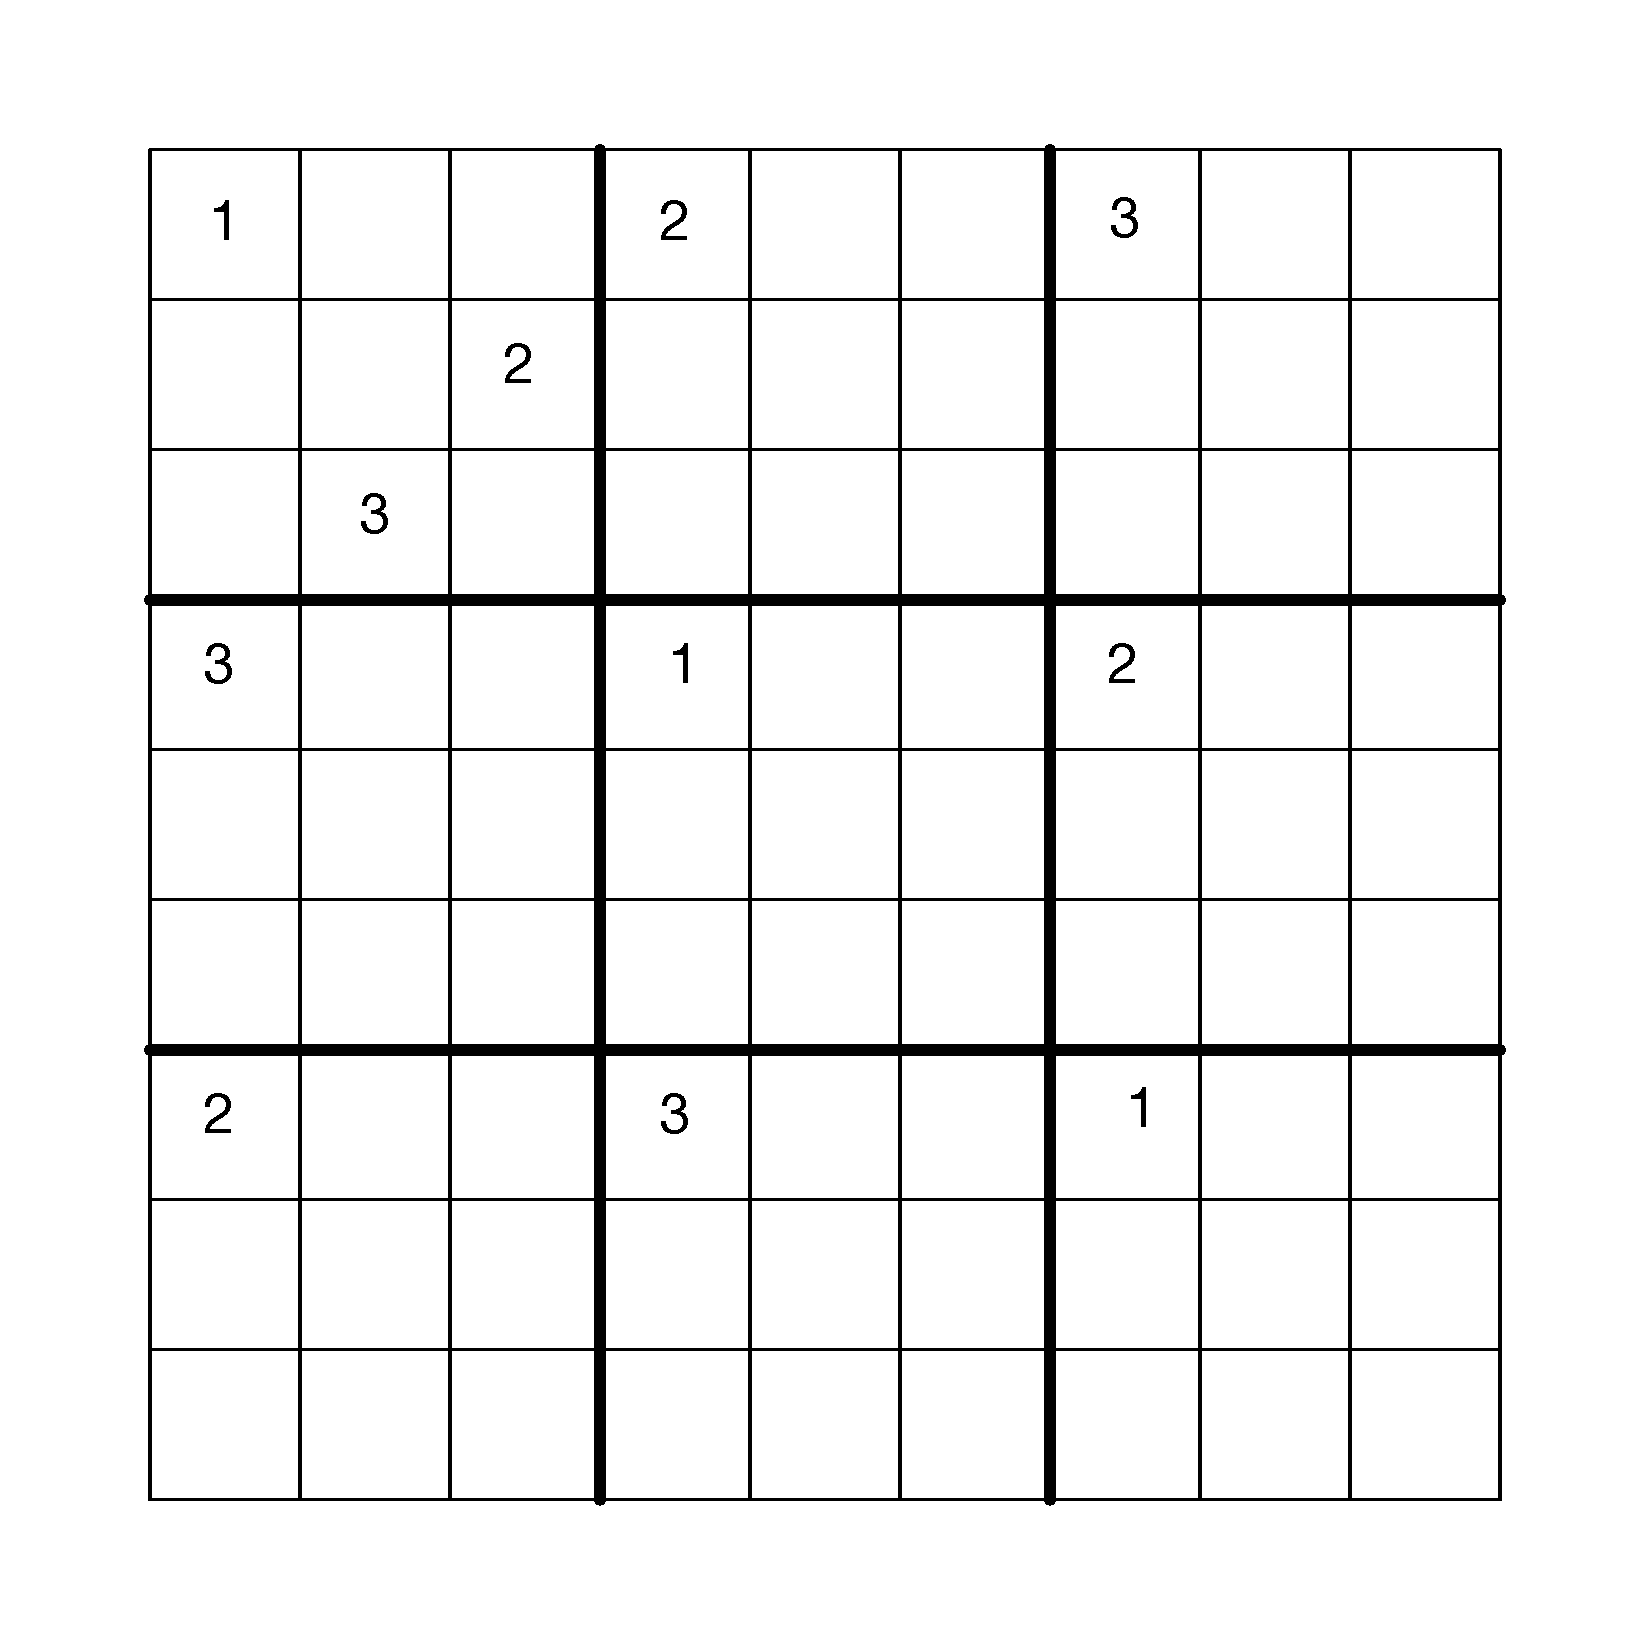
\includegraphics[width=0.45\textwidth]{figs/sudoku}
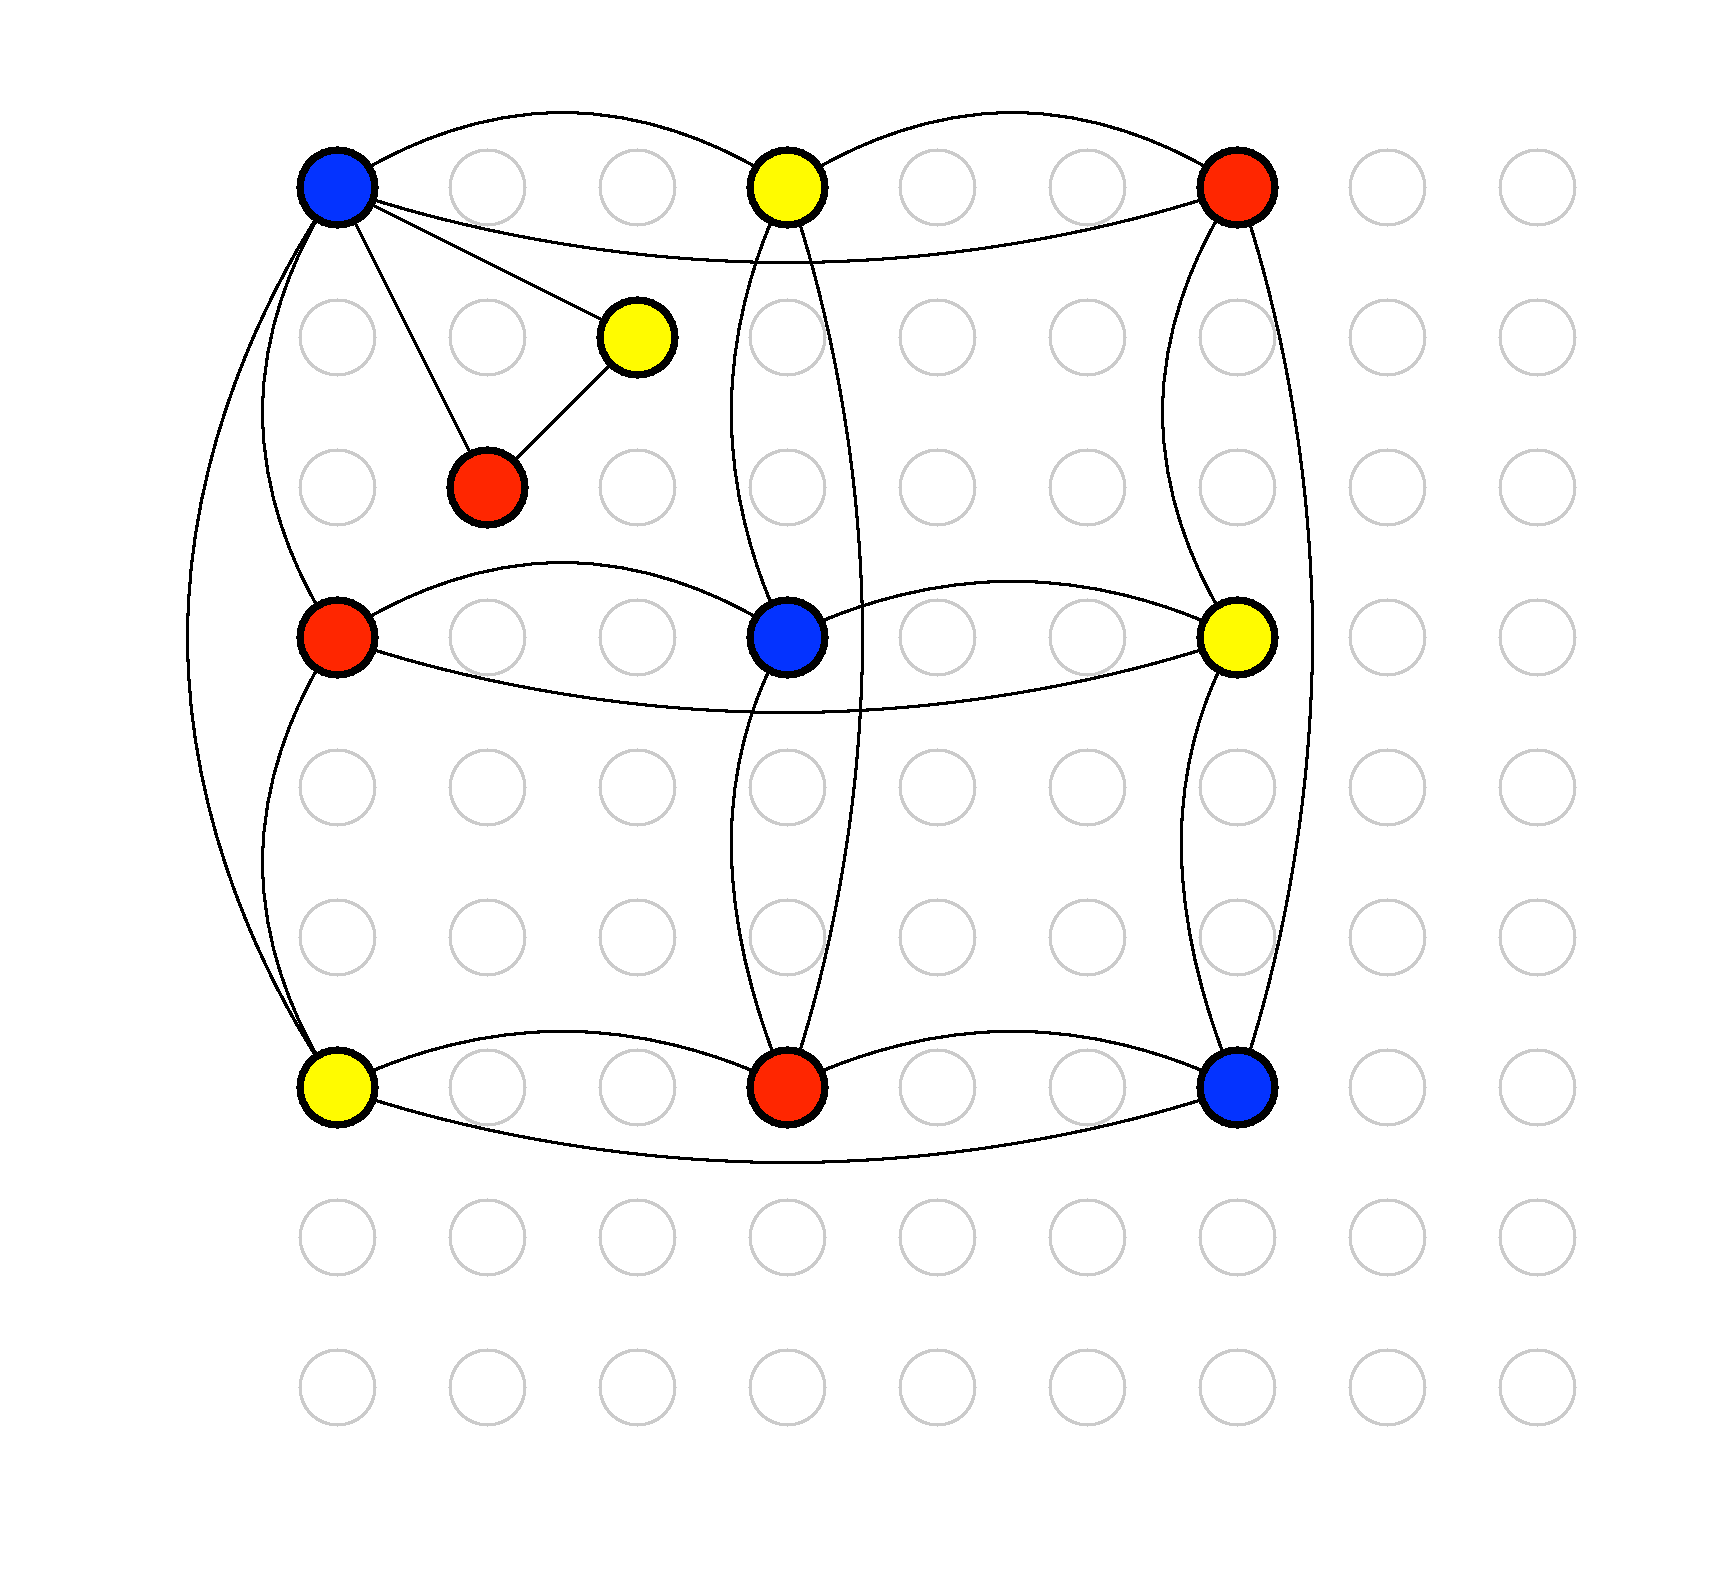
\includegraphics[width=0.5\textwidth]{figs/sudoku-graph}
\caption{A Sudoku game board and the corresponding colored graph.}
\label{fig:sudoku-graph}
\end{figure}


Given that Sudoku is graph coloring, one can use Sudoku strategies to
come up with an algorithm for allocating registers. For example, one
of the basic techniques for Sudoku is called Pencil Marks. The idea is
that you use a process of elimination to determine what numbers no
longer make sense for a square, and write down those numbers in the
square (writing very small). For example, if the number $1$ is
assigned to a square, then by process of elimination, you can write
the pencil mark $1$ in all the squares in the same row, column, and
region. Many Sudoku computer games provide automatic support for
Pencil Marks. This heuristic also reduces the degree of branching in
the search tree.

The Pencil Marks technique corresponds to the notion of color
\emph{saturation} due to \cite{Brelaz:1979eu}.  The saturation of a
node, in Sudoku terms, is the set of colors that are no longer
available. In graph terminology, we have the following definition:
\begin{equation*}
  \mathrm{saturation}(u) = \{ c \;|\; \exists v. v \in \mathrm{adjacent}(u)
     \text{ and } \mathrm{color}(v) = c \}
\end{equation*}
where $\mathrm{adjacent}(u)$ is the set of nodes adjacent to $u$.

Using the Pencil Marks technique leads to a simple strategy for
filling in numbers: if there is a square with only one possible number
left, then write down that number! But what if there are no squares
with only one possibility left? One brute-force approach is to just
make a guess. If that guess ultimately leads to a solution, great.  If
not, backtrack to the guess and make a different guess.  Of course,
backtracking can be horribly time consuming. One standard way to
reduce the amount of backtracking is to use the most-constrained-first
heuristic. That is, when making a guess, always choose a square with
the fewest possibilities left (the node with the highest saturation).
The idea is that choosing highly constrained squares earlier rather
than later is better because later there may not be any possibilities.

In some sense, register allocation is easier than Sudoku because we
can always cheat and add more numbers by mapping variables to the
stack. We say that a variable is \emph{spilled} when we decide to map
it to a stack location. We would like to minimize the time needed to
color the graph, and backtracking is expensive. Thus, it makes sense
to keep the most-constrained-first heuristic but drop the backtracking
in favor of greedy search (guess and just keep going).
Figure~\ref{fig:satur-algo} gives the pseudo-code for this simple
greedy algorithm for register allocation based on saturation and the
most-constrained-first heuristic, which is roughly equivalent to the
DSATUR algorithm of \cite{Brelaz:1979eu} (also known as saturation
degree ordering~\citep{Gebremedhin:1999fk,Omari:2006uq}).  Just
as in Sudoku, the algorithm represents colors with integers, with the
first $k$ colors corresponding to the $k$ registers in a given machine
and the rest of the integers corresponding to stack locations.

\begin{figure}[btp]
  \centering
\begin{lstlisting}[basicstyle=\rmfamily,deletekeywords={for,from,with,is,not,in,find},morekeywords={while},columns=fullflexible]
Algorithm: DSATUR
Input: a graph |$G$|
Output: an assignment |$\mathrm{color}[v]$| for each node |$v \in G$|

|$W \gets \mathit{vertices}(G)$|
while |$W \neq \emptyset$| do
    pick a node |$u$| from |$W$| with the highest saturation,
        breaking ties randomly
    find the lowest color |$c$| that is not in |$\{ \mathrm{color}[v] \;:\; v \in \mathrm{adjacent}(v)\}$|
    |$\mathrm{color}[u] \gets c$|
    |$W \gets W - \{u\}$|
\end{lstlisting}
  \caption{The saturation-based greedy graph coloring algorithm.}
  \label{fig:satur-algo}
\end{figure}

With this algorithm in hand, let us return to the running example and
consider how to color the interference graph in
Figure~\ref{fig:interfere}. We shall not use register \key{rax} for
register allocation because we use it to patch instructions, so we
remove that vertex from the graph.  Initially, all of the nodes are
not yet colored and they are unsaturated, so we annotate each of them
with a dash for their color and an empty set for the saturation.
\[
\begin{tikzpicture}[baseline=(current  bounding  box.center)]
\node (v) at (0,0)    {$v:-,\{\}$};
\node (w) at (3,0)    {$w:-,\{\}$};
\node (x) at (6,0)    {$x:-,\{\}$};
\node (y) at (3,-1.5) {$y:-,\{\}$};
\node (z) at (6,-1.5) {$z:-,\{\}$};
\node (t1) at (9,0)   {$t.1:-,\{\}$};
\node (t2) at (9,-1.5) {$t.2:-,\{\}$};

\draw (v) to (w);
\foreach \i in {w,x,y}
{
  \foreach \j in {w,x,y}
  {
    \draw (\i) to (\j);
  }
}
\draw (z) to (w);
\draw (z) to (y);
\draw (t1) to (z);
\draw (t2) to (t1);
\end{tikzpicture}
\]
We select a maximally saturated node and color it $0$. In this case we
have a 7-way tie, so we arbitrarily pick $y$. The then mark color $0$
as no longer available for $w$, $x$, and $z$ because they interfere
with $y$.
\[
\begin{tikzpicture}[baseline=(current  bounding  box.center)]
\node (v) at (0,0)    {$v:-,\{\}$};
\node (w) at (3,0)    {$w:-,\{0\}$};
\node (x) at (6,0)    {$x:-,\{0\}$};
\node (y) at (3,-1.5) {$y:0,\{\}$};
\node (z) at (6,-1.5) {$z:-,\{0\}$};
\node (t1) at (9,0)   {$t.1:-,\{\}$};
\node (t2) at (9,-1.5) {$t.2:-,\{\}$};
\draw (v) to (w);
\foreach \i in {w,x,y}
{
  \foreach \j in {w,x,y}
  {
    \draw (\i) to (\j);
  }
}
\draw (z) to (w);
\draw (z) to (y);
\draw (t1) to (z);
\draw (t2) to (t1);
\end{tikzpicture}
\]
Now we repeat the process, selecting another maximally saturated node.
This time there is a three-way tie between $w$, $x$, and $z$. We color
$w$ with $1$.
\[
\begin{tikzpicture}[baseline=(current  bounding  box.center)]
\node (v) at (0,0)    {$v:-,\{1\}$};
\node (w) at (3,0)    {$w:1,\{0\}$};
\node (x) at (6,0)    {$x:-,\{0,1\}$};
\node (y) at (3,-1.5) {$y:0,\{1\}$};
\node (z) at (6,-1.5) {$z:-,\{0,1\}$};
\node (t1) at (9,0)   {$t.1:-,\{\}$};
\node (t2) at (9,-1.5) {$t.2:-,\{\}$};
\draw (t1) to (z);
\draw (t2) to (t1);
\draw (v) to (w);
\foreach \i in {w,x,y}
{
  \foreach \j in {w,x,y}
  {
    \draw (\i) to (\j);
  }
}
\draw (z) to (w);
\draw (z) to (y);
\end{tikzpicture}
\]
The most saturated nodes are now $x$ and $z$. We color $x$ with the
next available color which is $2$.
\[
\begin{tikzpicture}[baseline=(current  bounding  box.center)]
\node (v) at (0,0)    {$v:-,\{1\}$};
\node (w) at (3,0)    {$w:1,\{0,2\}$};
\node (x) at (6,0)    {$x:2,\{0,1\}$};
\node (y) at (3,-1.5) {$y:0,\{1,2\}$};
\node (z) at (6,-1.5) {$z:-,\{0,1\}$};
\node (t1) at (9,0)   {$t.1:-,\{\}$};
\node (t2) at (9,-1.5) {$t.2:-,\{\}$};
\draw (t1) to (z);
\draw (t2) to (t1);
\draw (v) to (w);
\foreach \i in {w,x,y}
{
  \foreach \j in {w,x,y}
  {
    \draw (\i) to (\j);
  }
}
\draw (z) to (w);
\draw (z) to (y);
\end{tikzpicture}
\]
Node $z$ is the next most highly saturated, so we color $z$ with $2$.
\[
\begin{tikzpicture}[baseline=(current  bounding  box.center)]
\node (v) at (0,0)   {$v:-,\{1\}$};
\node (w) at (3,0)   {$w:1,\{0,2\}$};
\node (x) at (6,0)   {$x:2,\{0,1\}$};
\node (y) at (3,-1.5)  {$y:0,\{1,2\}$};
\node (z) at (6,-1.5)  {$z:2,\{0,1\}$};
\node (t1) at (9,0)   {$t.1:-,\{2\}$};
\node (t2) at (9,-1.5) {$t.2:-,\{\}$};
\draw (t1) to (z);
\draw (t2) to (t1);
\draw (v) to (w);
\foreach \i in {w,x,y}
{
  \foreach \j in {w,x,y}
  {
    \draw (\i) to (\j);
  }
}
\draw (z) to (w);
\draw (z) to (y);
\end{tikzpicture}
\]
We have a 2-way tie between $v$ and $t.1$. We choose to color $v$ with
$0$.
\[
\begin{tikzpicture}[baseline=(current  bounding  box.center)]
\node (v) at (0,0)   {$v:0,\{1\}$};
\node (w) at (3,0)   {$w:1,\{0,2\}$};
\node (x) at (6,0)   {$x:2,\{0,1\}$};
\node (y) at (3,-1.5)  {$y:0,\{1,2\}$};
\node (z) at (6,-1.5)  {$z:2,\{0,1\}$};
\node (t1) at (9,0)   {$t.1:-,\{2\}$};
\node (t2) at (9,-1.5) {$t.2:-,\{\}$};
\draw (t1) to (z);
\draw (t2) to (t1);
\draw (v) to (w);
\foreach \i in {w,x,y}
{
  \foreach \j in {w,x,y}
  {
    \draw (\i) to (\j);
  }
}
\draw (z) to (w);
\draw (z) to (y);
\end{tikzpicture}
\]
In the last two steps of the algorithm, we color $t.1$ with $0$
then $t.2$ with $1$.
\[
\begin{tikzpicture}[baseline=(current  bounding  box.center)]
\node (v) at (0,0)   {$v:0,\{1\}$};
\node (w) at (3,0)   {$w:1,\{0,2\}$};
\node (x) at (6,0)   {$x:2,\{0,1\}$};
\node (y) at (3,-1.5)  {$y:0,\{1,2\}$};
\node (z) at (6,-1.5)  {$z:2,\{0,1\}$};
\node (t1) at (9,0)   {$t.1:0,\{2,1\}$};
\node (t2) at (9,-1.5) {$t.2:1,\{0\}$};
\draw (t1) to (z);
\draw (t2) to (t1);
\draw (v) to (w);
\foreach \i in {w,x,y}
{
  \foreach \j in {w,x,y}
  {
    \draw (\i) to (\j);
  }
}
\draw (z) to (w);
\draw (z) to (y);
\end{tikzpicture}
\]


With the coloring complete, we can finalize the assignment of
variables to registers and stack locations. Recall that if we have $k$
registers, we map the first $k$ colors to registers and the rest to
stack locations.  Suppose for the moment that we just have one extra
register to use for register allocation, just \key{rbx}. Then the
following is the mapping of colors to registers and stack allocations.
\[
  \{ 0 \mapsto \key{\%rbx}, \; 1 \mapsto \key{-8(\%rbp)}, \; 2 \mapsto \key{-16(\%rbp)}, \ldots \}
\]
Putting this mapping together with the above coloring of the variables, we
arrive at the assignment:
\begin{gather*}
  \{ v \mapsto \key{\%rbx}, \,
  w \mapsto \key{-8(\%rbp)},  \,
  x \mapsto \key{-16(\%rbp)}, \,
  y \mapsto \key{\%rbx},  \,
  z\mapsto \key{-16(\%rbp)}, \\
  t.1\mapsto \key{\%rbx} ,\,
  t.2\mapsto \key{-8(\%rbp)} \}
\end{gather*}
Applying this assignment to our running example
(Figure~\ref{fig:reg-eg}) yields the program on the right.\\
% why frame size of 32? -JGS
\begin{minipage}{0.4\textwidth}
\begin{lstlisting}
  (program (v w x y z)
    (movq (int 1) (var v))
    (movq (int 46) (var w))
    (movq (var v) (var x))
    (addq (int 7) (var x))
    (movq (var x) (var y))
    (addq (int 4) (var y))
    (movq (var x) (var z))
    (addq (var w) (var z))
    (movq (var y) (var t.1))
    (negq (var t.1))
    (movq (var z) (var t.2))
    (addq (var t.1) (var t.2))
    (movq (var t.2) (reg rax)))
\end{lstlisting}
\end{minipage}
$\Rightarrow$
\begin{minipage}{0.45\textwidth}
\begin{lstlisting}
(program 16
  (movq (int 1) (reg rbx))
  (movq (int 46) (deref rbp -8))
  (movq (reg rbx) (deref rbp -16))
  (addq (int 7) (deref rbp -16))
  (movq (deref rbp -16) (reg rbx))
  (addq (int 4) (reg rbx))
  (movq (deref rbp -16) (deref rbp -16))
  (addq (deref rbp -8) (deref rbp -16))
  (movq (reg rbx) (reg rbx))
  (negq (reg rbx))
  (movq (deref rbp -16) (deref rbp -8))
  (addq (reg rbx) (deref rbp -8))
  (movq (deref rbp -8) (reg rax)))
\end{lstlisting}
\end{minipage}

The resulting program is almost an x86 program. The remaining step
is to apply the patch instructions pass. In this example, the trivial
move of \code{-16(\%rbp)} to itself is deleted and the addition of
\code{-8(\%rbp)} to \key{-16(\%rbp)} is fixed by going through
\code{rax}. The following shows the portion of the program that
changed.
\begin{lstlisting}
  (addq (int 4) (reg rbx))
  (movq (deref rbp -8) (reg rax)
  (addq (reg rax) (deref rbp -16))
\end{lstlisting}
An overview of all of the passes involved in register allocation is
shown in Figure~\ref{fig:reg-alloc-passes}.

\begin{figure}[p]
\begin{tikzpicture}[baseline=(current  bounding  box.center)]
\node (R1) at (0,2)  {\large $R_1$};
\node (R1-2) at (3,2)  {\large $R_1$};
\node (C0-1) at (3,0)  {\large $C_0$};

\node (x86-2) at (3,-2)  {\large $\text{x86}^{*}$};
\node (x86-3) at (6,-2)  {\large $\text{x86}^{*}$};
\node (x86-4) at (9,-2) {\large $\text{x86}$};
\node (x86-5) at (12,-2) {\large $\text{x86}^{\dagger}$};

\node (x86-2-1) at (3,-4)  {\large $\text{x86}^{*}$};
\node (x86-2-2) at (6,-4)  {\large $\text{x86}^{*}$};

\path[->,bend left=15] (R1) edge [above] node {\ttfamily\footnotesize uniquify} (R1-2);
\path[->,bend left=15] (R1-2) edge [right] node {\ttfamily\footnotesize flatten} (C0-1);
\path[->,bend right=15] (C0-1) edge [left] node {\ttfamily\footnotesize select-instr.} (x86-2);
\path[->,bend left=15] (x86-2) edge [right] node {\ttfamily\footnotesize\color{red} uncover-live} (x86-2-1);
\path[->,bend right=15] (x86-2-1) edge [below] node {\ttfamily\footnotesize\color{red} build-inter.} (x86-2-2);
\path[->,bend right=15] (x86-2-2) edge [right] node {\ttfamily\footnotesize\color{red} allocate-reg.} (x86-3);
\path[->,bend left=15] (x86-3) edge [above] node {\ttfamily\footnotesize patch-instr.} (x86-4);
\path[->,bend left=15] (x86-4) edge [above] node {\ttfamily\footnotesize print-x86} (x86-5);
\end{tikzpicture}
\caption{Diagram of the passes for $R_1$ with register allocation.}
\label{fig:reg-alloc-passes}
\end{figure}

\begin{exercise}\normalfont
Implement the pass \code{allocate-registers} and test it by creating
new example programs that exercise all of the register allocation
algorithm, such as forcing variables to be spilled to the stack.

I recommend organizing our code by creating a helper function named
\code{color-graph} that takes an interference graph and a list of all
the variables in the program. This function should return a mapping of
variables to their colors. By creating this helper function, we will
be able to reuse it in Chapter~\ref{ch:functions} when we add support
for functions.  Once you have obtained the coloring from
\code{color-graph}, you can assign the variables to registers or stack
locations based on their color and then use the \code{assign-homes}
function from Section~\ref{sec:assign-s0} to replace the variables
with their assigned location.
\end{exercise}


\section{Print x86 and Conventions for Registers}
\label{sec:print-x86-reg-alloc}

Recall the the \code{print-x86} pass generates the prelude and
conclusion instructions for the \code{main} function.  The prelude
saved the values in \code{rbp} and \code{rsp} and the conclusion
returned those values to \code{rbp} and \code{rsp}. The reason for
this is that there are agreed-upon conventions for how different
functions share the same fixed set of registers. There is a function
inside the operating system (OS) that calls our \code{main} function,
and that OS function uses the same registers that we use in
\code{main}. The convention for x86 is that the caller is responsible
for freeing up some registers, the \emph{caller save registers}, prior
to the function call, and the callee is responsible for saving and
restoring some other registers, the \emph{callee save registers},
before and after using them. The caller save registers are
\begin{lstlisting}
  rax rdx rcx rsi rdi r8 r9 r10 r11
\end{lstlisting}
while the callee save registers are
\begin{lstlisting}
  rsp rbp rbx r12 r13 r14 r15
\end{lstlisting}
Another way to think about this caller/callee convention is the
following. The caller should assume that all the caller save registers
get overwritten with arbitrary values by the callee.  On the other
hand, the caller can safely assume that all the callee save registers
contain the same values after the call that they did before the call.
The callee can freely use any of the caller save registers.  However,
if the callee wants to use a callee save register, the callee must
arrange to put the original value back in the register prior to
returning to the caller, which is usually accomplished by saving and
restoring the value from the stack.

The upshot of these conventions is that the \code{main} function needs
to save (in the prelude) and restore (in the conclusion) any callee
save registers that get used during register allocation. The simplest
approach is to save and restore all the callee save registers. The
more efficient approach is to keep track of which callee save
registers were used and only save and restore them. Either way, make
sure to take this use of stack space into account when you round up
the size of the frame to make sure it is a multiple of 16 bytes.

\section{Challenge: Move Biasing$^{*}$}
\label{sec:move-biasing}

This section describes an optional enhancement to register allocation
for those students who are looking for an extra challenge or who have
a deeper interest in register allocation.

We return to the running example, but we remove the supposition that
we only have one register to use. So we have the following mapping of
color numbers to registers.
\[
  \{ 0 \mapsto \key{\%rbx}, \; 1 \mapsto \key{\%rcx}, \; 2 \mapsto \key{\%rdx}, \ldots \}
\]
Using the same assignment that was produced by register allocator
described in the last section, we get the following program.

\begin{minipage}{0.45\textwidth}
\begin{lstlisting}
  (program (v w x y z)
    (movq (int 1) (var v))
    (movq (int 46) (var w))
    (movq (var v) (var x))
    (addq (int 7) (var x))
    (movq (var x) (var y))
    (addq (int 4) (var y))
    (movq (var x) (var z))
    (addq (var w) (var z))
    (movq (var y) (var t.1))
    (negq (var t.1))
    (movq (var z) (var t.2))
    (addq (var t.1) (var t.2))
    (movq (var t.2) (reg rax)))
\end{lstlisting}
\end{minipage}
$\Rightarrow$
\begin{minipage}{0.45\textwidth}
\begin{lstlisting}
(program 0
  (movq (int 1) (reg rbx))
  (movq (int 46) (reg rcx))
  (movq (reg rbx) (reg rdx))
  (addq (int 7) (reg rdx))
  (movq (reg rdx) (reg rbx))
  (addq (int 4) (reg rbx))
  (movq (reg rdx) (reg rdx))
  (addq (reg rcx) (reg rdx))
  (movq (reg rbx) (reg rbx))
  (negq (reg rbx))
  (movq (reg rdx) (reg rcx))
  (addq (reg rbx) (reg rcx))
  (movq (reg rcx) (reg rax)))
\end{lstlisting}
\end{minipage}

While this allocation is quite good, we could do better. For example,
the variables \key{v} and \key{x} ended up in different registers, but
if they had been placed in the same register, then the move from
\key{v} to \key{x} could be removed.

We say that two variables $p$ and $q$ are \emph{move related} if they
participate together in a \key{movq} instruction, that is, \key{movq
  p, q} or \key{movq q, p}. When the register allocator chooses a
color for a variable, it should prefer a color that has already been
used for a move-related variable (assuming that they do not
interfere). Of course, this preference should not override the
preference for registers over stack locations, but should only be used
as a tie breaker when choosing between registers or when choosing
between stack locations.

We recommend that you represent the move relationships in a graph,
similar to how we represented interference.  The following is the
\emph{move graph} for our running example.
\[
\begin{tikzpicture}[baseline=(current  bounding  box.center)]
\node (v) at (0,0)    {$v$};
\node (w) at (3,0)    {$w$};
\node (x) at (6,0)    {$x$};
\node (y) at (3,-1.5) {$y$};
\node (z) at (6,-1.5) {$z$};
\node (t1) at (9,0)   {$t.1$};
\node (t2) at (9,-1.5) {$t.2$};
\draw (t1) to (y);
\draw (t2) to (z);
\draw[bend left=20] (v) to (x);
\draw (x) to (y);
\draw (x) to (z);
\end{tikzpicture}
\]

Now we replay the graph coloring, pausing to see the coloring of $z$
and $v$. So we have the following coloring so far and the most
saturated vertex is $z$.
\[
\begin{tikzpicture}[baseline=(current  bounding  box.center)]
\node (v) at (0,0)    {$v:-,\{1\}$};
\node (w) at (3,0)    {$w:1,\{0,2\}$};
\node (x) at (6,0)    {$x:2,\{0,1\}$};
\node (y) at (3,-1.5) {$y:0,\{1,2\}$};
\node (z) at (6,-1.5) {$z:-,\{0,1\}$};
\node (t1) at (9,0)   {$t.1:-,\{\}$};
\node (t2) at (9,-1.5) {$t.2:-,\{\}$};
\draw (t1) to (z);
\draw (t2) to (t1);
\draw (v) to (w);
\foreach \i in {w,x,y}
{
  \foreach \j in {w,x,y}
  {
    \draw (\i) to (\j);
  }
}
\draw (z) to (w);
\draw (z) to (y);
\end{tikzpicture}
\]
Last time we chose to color $z$ with $2$, which so happens to be the
color of $x$, and $z$ is move related to $x$. This was rather lucky,
and if the program had been a little different, and say $x$ had been
already assigned to $3$, then $z$ would still get $2$ and our luck
would have run out. With move biasing, we use the fact that $z$ and
$x$ are move related to influence the choice of color for $z$, in this
case choosing $2$ because that's the color of $x$.
\[
\begin{tikzpicture}[baseline=(current  bounding  box.center)]
\node (v) at (0,0)    {$v:-,\{1\}$};
\node (w) at (3,0)    {$w:1,\{0,2\}$};
\node (x) at (6,0)    {$x:2,\{0,1\}$};
\node (y) at (3,-1.5) {$y:0,\{1,2\}$};
\node (z) at (6,-1.5) {$z:2,\{0,1\}$};
\node (t1) at (9,0)   {$t.1:-,\{2\}$};
\node (t2) at (9,-1.5) {$t.2:-,\{\}$};
\draw (t1) to (z);
\draw (t2) to (t1);
\draw (v) to (w);
\foreach \i in {w,x,y}
{
  \foreach \j in {w,x,y}
  {
    \draw (\i) to (\j);
  }
}
\draw (z) to (w);
\draw (z) to (y);
\end{tikzpicture}
\]

Next we consider coloring the variable $v$, and we just need to avoid
choosing $1$ because of the interference with $w$. Last time we choose
the color $0$, simply because it was the lowest, but this time we know
that $v$ is move related to $x$, so we choose the color $2$.
\[
\begin{tikzpicture}[baseline=(current  bounding  box.center)]
\node (v) at (0,0)    {$v:2,\{1\}$};
\node (w) at (3,0)    {$w:1,\{0,2\}$};
\node (x) at (6,0)    {$x:2,\{0,1\}$};
\node (y) at (3,-1.5) {$y:0,\{1,2\}$};
\node (z) at (6,-1.5) {$z:2,\{0,1\}$};
\node (t1) at (9,0)   {$t.1:-,\{2\}$};
\node (t2) at (9,-1.5) {$t.2:-,\{\}$};
\draw (t1) to (z);
\draw (t2) to (t1);
\draw (v) to (w);
\foreach \i in {w,x,y}
{
  \foreach \j in {w,x,y}
  {
    \draw (\i) to (\j);
  }
}
\draw (z) to (w);
\draw (z) to (y);
\end{tikzpicture}
\]

We apply this register assignment to the running example, on the left,
to obtain the code on right.

\begin{minipage}{0.45\textwidth}
\begin{lstlisting}
  (program (v w x y z)
    (movq (int 1) (var v))
    (movq (int 46) (var w))
    (movq (var v) (var x))
    (addq (int 7) (var x))
    (movq (var x) (var y))
    (addq (int 4) (var y))
    (movq (var x) (var z))
    (addq (var w) (var z))
    (movq (var y) (var t.1))
    (negq (var t.1))
    (movq (var z) (var t.2))
    (addq (var t.1) (var t.2))
    (movq (var t.2) (reg rax)))
\end{lstlisting}
\end{minipage}
$\Rightarrow$
\begin{minipage}{0.45\textwidth}
\begin{lstlisting}
(program 0
  (movq (int 1) (reg rdx))
  (movq (int 46) (reg rcx))
  (movq (reg rdx) (reg rdx))
  (addq (int 7) (reg rdx))
  (movq (reg rdx) (reg rbx))
  (addq (int 4) (reg rbx))
  (movq (reg rdx) (reg rdx))
  (addq (reg rcx) (reg rdx))
  (movq (reg rbx) (reg rbx))
  (negq (reg rbx))
  (movq (reg rdx) (reg rcx))
  (addq (reg rbx) (reg rcx))
  (movq (reg rcx) (reg rax)))
\end{lstlisting}
\end{minipage}

The \code{patch-instructions} then removes the trivial moves from
\key{v} to \key{x}, from \key{x} to \key{z}, and from \key{y} to
\key{t.1}, to obtain the following result.
\begin{lstlisting}
(program 0
  (movq (int 1) (reg rdx))
  (movq (int 46) (reg rcx))
  (addq (int 7) (reg rdx))
  (movq (reg rdx) (reg rbx))
  (addq (int 4) (reg rbx))
  (addq (reg rcx) (reg rdx))
  (negq (reg rbx))
  (movq (reg rdx) (reg rcx))
  (addq (reg rbx) (reg rcx))
  (movq (reg rcx) (reg rax)))
\end{lstlisting}

\begin{exercise}\normalfont
Change your implementation of \code{allocate-registers} to take move
biasing into account. Make sure that your compiler still passes all of
the previous tests. Create two new tests that include at least one
opportunity for move biasing and visually inspect the output x86
programs to make sure that your move biasing is working properly.
\end{exercise}

\margincomment{\footnotesize To do: another neat challenge would be to do
  live range splitting~\citep{Cooper:1998ly}. \\ --Jeremy}


%%%%%%%%%%%%%%%%%%%%%%%%%%%%%%%%%%%%%%%%%%%%%%%%%%%%%%%%%%%%%%%%%%%%%%%%%%%%%%%%
\chapter{Booleans, Control Flow, and Type Checking}
\label{ch:bool-types}

The $R_0$ and $R_1$ languages only had a single kind of value, the
integers. In this Chapter we add a second kind of value, the Booleans,
to create the $R_2$ language. The Boolean values \emph{true} and
\emph{false} are written \key{\#t} and \key{\#f} respectively in
Racket.  We also introduce several operations that involve Booleans
(\key{and}, \key{not}, \key{eq?}, \key{<}, etc.) and the conditional
\key{if} expression. With the addition of \key{if} expressions,
programs can have non-trivial control flow which has an impact on
several parts of the compiler. Also, because we now have two kinds of
values, we need to worry about programs that apply an operation to the
wrong kind of value, such as \code{(not 1)}.

There are two language design options for such situations.  One option
is to signal an error and the other is to provide a wider
interpretation of the operation. The Racket language uses a mixture of
these two options, depending on the operation and the kind of
value. For example, the result of \code{(not 1)} in Racket is
\code{\#f} because Racket treats non-zero integers like \code{\#t}. On
the other hand, \code{(car 1)} results in a run-time error in Racket
stating that \code{car} expects a pair.

The Typed Racket language makes similar design choices as Racket,
except much of the error detection happens at compile time instead of
run time. Like Racket, Typed Racket accepts and runs \code{(not 1)},
producing \code{\#f}. But in the case of \code{(car 1)}, Typed Racket
reports a compile-time error because the type of the argument is
expected to be of the form \code{(Listof T)} or \code{(Pairof T1 T2)}.

For the $R_2$ language we choose to be more like Typed Racket in that
we shall perform type checking during compilation. In
Chapter~\ref{ch:type-dynamic} we study the alternative choice, that
is, how to compile a dynamically typed language like Racket.  The
$R_2$ language is a subset of Typed Racket but by no means includes
all of Typed Racket. Furthermore, for many of the operations we shall
take a narrower interpretation than Typed Racket, for example,
rejecting \code{(not 1)}.

This chapter is organized as follows.  We begin by defining the syntax
and interpreter for the $R_2$ language (Section~\ref{sec:r2-lang}). We
then introduce the idea of type checking and build a type checker for
$R_2$ (Section~\ref{sec:type-check-r2}). To compile $R_2$ we need to
enlarge the intermediate language $C_0$ into $C_1$, which we do in
Section~\ref{sec:c1}. The remaining sections of this Chapter discuss
how our compiler passes need to change to accommodate Booleans and
conditional control flow.


\section{The $R_2$ Language}
\label{sec:r2-lang}

The syntax of the $R_2$ language is defined in
Figure~\ref{fig:r2-syntax}. It includes all of $R_1$ (shown in gray) ,
the Boolean literals \code{\#t} and \code{\#f}, and the conditional
\code{if} expression. Also, we expand the operators to include the
\key{and} and \key{not} on Booleans, the \key{eq?}  operations for
comparing two integers or two Booleans, and the \key{<}, \key{<=},
\key{>}, and \key{>=} operations for comparing integers.

\begin{figure}[tp]
\centering
\fbox{
\begin{minipage}{0.96\textwidth}
\[
\begin{array}{lcl}
  \itm{cmp} &::= & \key{eq?} \mid \key{<} \mid \key{<=} \mid \key{>} \mid \key{>=} \\
  \Exp &::=& \gray{\Int \mid (\key{read}) \mid (\key{-}\;\Exp) \mid (\key{+} \; \Exp\;\Exp)}  \\
     &\mid&  \gray{\Var \mid \LET{\Var}{\Exp}{\Exp}} \\
     &\mid& \key{\#t} \mid \key{\#f} \mid
      (\key{and}\;\Exp\;\Exp) \mid (\key{not}\;\Exp) \\
      &\mid& (\itm{cmp}\;\Exp\;\Exp) \mid \IF{\Exp}{\Exp}{\Exp} \\
  R_2 &::=& (\key{program} \; \Exp)
\end{array}
\]
\end{minipage}
}
\caption{The syntax of $R_2$, extending $R_1$ with Booleans and
  conditionals.}
\label{fig:r2-syntax}
\end{figure}

Figure~\ref{fig:interp-R2} defines the interpreter for $R_2$, omitting
the parts that are the same as the interpreter for $R_1$
(Figure~\ref{fig:interp-R1}). The literals \code{\#t} and \code{\#f}
simply evaluate to themselves. The conditional expression $(\key{if}\,
\itm{cnd}\,\itm{thn}\,\itm{els})$ evaluates the Boolean expression
\itm{cnd} and then either evaluates \itm{thn} or \itm{els} depending
on whether \itm{cnd} produced \code{\#t} or \code{\#f}. The logical
operations \code{not} and \code{and} behave as you might expect, but
note that the \code{and} operation is short-circuiting. That is, given
the expression $(\key{and}\,e_1\,e_2)$, the expression $e_2$ is not
evaluated if $e_1$ evaluates to \code{\#f}.

With the addition of the comparison operations, there are quite a few
primitive operations and the interpreter code for them is somewhat
repetitive. In Figure~\ref{fig:interp-R2} we factor out the different
parts into the \code{interp-op} function and the similar parts into
the one match clause shown in Figure~\ref{fig:interp-R2}. It is
important for that match clause to come last because it matches
\emph{any} compound S-expression.  We do not use \code{interp-op} for
the \code{and} operation because of the short-circuiting behavior in
the order of evaluation of its arguments.


\begin{figure}[tbp]
\begin{lstlisting}
    (define primitives (set '+ '- 'eq? '< '<= '> '>= 'not 'read))

    (define (interp-op op)
      (match op
         ['+ fx+]
         ['- (lambda (n) (fx- 0 n))]
         ['not (lambda (v) (match v [#t #f] [#f #t]))]
	 ['read read-fixnum]
         ['eq? (lambda (v1 v2)
                 (cond [(or (and (fixnum? v1) (fixnum? v2))
                            (and (boolean? v1) (boolean? v2))
                            (and (vector? v1) (vector? v2)))
                        (eq? v1 v2)]))]
         ['< (lambda (v1 v2)
                 (cond [(and (fixnum? v1) (fixnum? v2))
                        (< v1 v2)]))]
         ['<= (lambda (v1 v2)
                 (cond [(and (fixnum? v1) (fixnum? v2))
                        (<= v1 v2)]))]
         ['> (lambda (v1 v2)
                 (cond [(and (fixnum? v1) (fixnum? v2))
                        (<= v1 v2)]))]
         ['>= (lambda (v1 v2)
                 (cond [(and (fixnum? v1) (fixnum? v2))
                        (<= v1 v2)]))]
	 [else (error 'interp-op "unknown operator")]))

   (define (interp-R2 env)
     (lambda (e)
       (define recur (interp-R2 env))
       (match e
         ...
         [(? boolean?) e]
         [`(if ,(app recur cnd) ,thn ,els)
          (match cnd
            [#t (recur thn)]
            [#f (recur els)])]
         [`(not ,(app recur v))
          (match v [#t #f] [#f #t])]
         [`(and ,(app recur v1) ,e2)
           (match v1
             [#t (match (recur e2) [#t #t] [#f #f])]
             [#f #f])]
         [`(,op ,(app recur args) ...)
           #:when (set-member? primitives op)
           (apply (interp-op op) args)]
         )))
\end{lstlisting}
\caption{Interpreter for the $R_2$ language.}
\label{fig:interp-R2}
\end{figure}


\section{Type Checking $R_2$ Programs}
\label{sec:type-check-r2}

It is helpful to think about type checking into two complementary
ways. A type checker predicts the \emph{type} of value that will be
produced by each expression in the program.  For $R_2$, we have just
two types, \key{Integer} and \key{Boolean}. So a type checker should
predict that
\begin{lstlisting}
   (+ 10 (- (+ 12 20)))
\end{lstlisting}
produces an \key{Integer} while
\begin{lstlisting}
   (and (not #f) #t)
\end{lstlisting}
produces a \key{Boolean}.

As mentioned at the beginning of this chapter, a type checker also
rejects programs that apply operators to the wrong type of value. Our
type checker for $R_2$ will signal an error for the following
expression because, as we have seen above, the expression \code{(+ 10
  ...)} has type \key{Integer}, and we require the argument of a
\code{not} to have type \key{Boolean}.
\begin{lstlisting}
   (not (+ 10 (- (+ 12 20))))
\end{lstlisting}

The type checker for $R_2$ is best implemented as a structurally
recursive function over the AST. Figure~\ref{fig:type-check-R2} shows
many of the clauses for the \code{typecheck-R2} function.  Given an
input expression \code{e}, the type checker either returns the type
(\key{Integer} or \key{Boolean}) or it signals an error.  Of course,
the type of an integer literal is \code{Integer} and the type of a
Boolean literal is \code{Boolean}.  To handle variables, the type
checker, like the interpreter, uses an association list. However, in
this case the association list maps variables to types instead of
values. Consider the clause for \key{let}.  We type check the
initializing expression to obtain its type \key{T} and then associate
type \code{T} with the variable \code{x}. When the type checker
encounters the use of a variable, it can lookup its type in the
association list.

\begin{figure}[tbp]
\begin{lstlisting}
   (define (typecheck-R2 env)
     (lambda (e)
       (define recur (typecheck-R2 env e))
       (match e
         [(? fixnum?)  'Integer]
         [(? boolean?) 'Boolean]
         [(? symbol?)  (lookup e env)]
         [`(read)      'Integer]
         [`(let ([,x ,(app recur T)]) ,body)
          (define new-env (cons (cons x T) env))
          (typecheck-R2 new-env body)]
         ...
         [`(not ,(app (typecheck-R2 env) T))
          (match T
            ['Boolean 'Boolean]
            [else (error 'typecheck-R2 "'not' expects a Boolean" e)])]
         ...
         [`(program ,body)
          (define ty ((typecheck-R2 '()) body))
          `(program (type ,ty) ,body)]
         )))
\end{lstlisting}
\caption{Skeleton of a type checker for the $R_2$ language.}
\label{fig:type-check-R2}
\end{figure}

To print the resulting value correctly, the overall type of the
program must be threaded through the remainder of the passes. We can
store the type within the \key{program} form as shown in Figure
\ref{fig:type-check-R2}. The syntax for post-typechecking $R_2$
programs as follows: \\
\fbox{
\begin{minipage}{0.87\textwidth}
\[
\begin{array}{lcl}
  R_2 &::=& (\key{program}\;(\key{type}\;\itm{type})\; \Exp)
\end{array}
\]
\end{minipage}
}

\begin{exercise}\normalfont
Complete the implementation of \code{typecheck-R2} and test it on 10
new example programs in $R_2$ that you choose based on how thoroughly
they test the type checking algorithm. Half of the example programs
should have a type error, to make sure that your type checker properly
rejects them. The other half of the example programs should not have
type errors. Your testing should check that the result of the type
checker agrees with the value returned by the interpreter, that is, if
the type checker returns \key{Integer}, then the interpreter should
return an integer. Likewise, if the type checker returns
\key{Boolean}, then the interpreter should return \code{\#t} or
\code{\#f}. Note that if your type checker does not signal an error
for a program, then interpreting that program should not encounter an
error.  If it does, there is something wrong with your type checker.
\end{exercise}

\section{The $C_1$ Language}
\label{sec:c1}

The $R_2$ language adds Booleans and conditional expressions to $R_1$.
As with $R_1$, we shall compile to a C-like intermediate language, but
we need to grow that intermediate language to handle the new features
in $R_2$. Figure~\ref{fig:c1-syntax} shows the new features of $C_1$;
we add logic and comparison operators to the $\Exp$ non-terminal, the
literals \key{\#t} and \key{\#f} to the $\Arg$ non-terminal, and we
add an \key{if} statement. The \key{if} statement of $C_1$ includes an
\key{eq?} test, which is needed for improving code generation in
Section~\ref{sec:opt-if}.  We do not include \key{and} in $C_1$
because it is not needed in the translation of the \key{and} of $R_2$.

\begin{figure}[tp]
\fbox{
\begin{minipage}{0.96\textwidth}
\[
\begin{array}{lcl}
\Arg &::=& \gray{\Int \mid \Var} \mid \key{\#t} \mid \key{\#f} \\
\itm{cmp} &::= & \key{eq?} \mid \key{<} \mid \key{<=} \mid \key{>} \mid \key{>=} \\
\Exp &::= & \gray{\Arg \mid (\key{read}) \mid (\key{-}\;\Arg) \mid (\key{+} \; \Arg\;\Arg)}
      \mid (\key{not}\;\Arg) \mid (\itm{cmp}\;\Arg\;\Arg) \\
\Stmt &::=& \gray{\ASSIGN{\Var}{\Exp} \mid \RETURN{\Arg}} \\
      &\mid& \IF{(\itm{cmp}\, \Arg\,\Arg)}{\Stmt^{*}}{\Stmt^{*}} \\
C_1 & ::= & (\key{program}\;(\Var^{*})\;(\key{type}\;\textit{type})\;\Stmt^{+})
\end{array}
\]
\end{minipage}
}
\caption{The $C_1$ language, extending $C_0$ with Booleans and conditionals.}
\label{fig:c1-syntax}
\end{figure}

\section{Flatten Expressions}
\label{sec:flatten-r2}

We expand the \code{flatten} pass to handle the Boolean literals
\key{\#t} and \key{\#f}, the new logic and comparison operations, and
\key{if} expressions. We shall start with a simple example of
translating a \key{if} expression, shown below on the left. \\
\begin{tabular}{lll}
\begin{minipage}{0.4\textwidth}
\begin{lstlisting}
 (program (if #f 0 42))
\end{lstlisting}
\end{minipage}
&
$\Rightarrow$
&
\begin{minipage}{0.4\textwidth}
\begin{lstlisting}
(program (if.1)
  (if (eq? #t #f)
    ((assign if.1 0))
    ((assign if.1 42)))
  (return if.1))
\end{lstlisting}
\end{minipage}
\end{tabular} \\
The value of the \key{if} expression is the value of the branch that
is selected. Recall that in the \code{flatten} pass we need to replace
arbitrary expressions with $\Arg$'s (variables or literals). In the
translation above, on the right, we have replaced the \key{if}
expression with a new variable \key{if.1}, inside \code{(return
  if.1)}, and we have produced code that will assign the appropriate
value to \key{if.1} using an \code{if} statement prior to the
\code{return}.  For $R_1$, the \code{flatten} pass returned a list of
assignment statements. Here, for $R_2$, we return a list of statements
that can include both \key{if} statements and assignment statements.

The next example is a bit more involved, showing what happens when
there are complex expressions (not variables or literals) in the
condition and branch expressions of an \key{if}, including nested
\key{if} expressions.

\begin{tabular}{lll}
\begin{minipage}{0.4\textwidth}
\begin{lstlisting}
(program
  (if (eq? (read) 0)
      777
      (+ 2 (if (eq? (read) 0)
               40
               444))))
\end{lstlisting}
\end{minipage}
&
$\Rightarrow$
&
\begin{minipage}{0.4\textwidth}
\begin{lstlisting}
(program (t.1 t.2 if.1 t.3 t.4
           if.2 t.5)
  (assign t.1 (read))
  (assign t.2 (eq? t.1 0))
  (if (eq? #t t.2)
    ((assign if.1 777))
    ((assign t.3 (read))
     (assign t.4 (eq? t.3 0))
     (if (eq? #t t.4)
       ((assign if.2 40))
       ((assign if.2 444)))
     (assign t.5 (+ 2 if.2))
     (assign if.1 t.5)))
  (return if.1))
\end{lstlisting}
\end{minipage}
\end{tabular} \\

The \code{flatten} clauses for the Boolean literals and the operations
\key{not} and \key{eq?} are straightforward.  However, the
\code{flatten} clause for \key{and} requires some care to properly
imitate the order of evaluation of the interpreter for $R_2$
(Figure~\ref{fig:interp-R2}). We recommend using an \key{if} statement
in the code you generate for \key{and}.

The \code{flatten} clause for \key{if} also requires some care because
the condition of the \key{if} can be an arbitrary expression in $R_2$,
but in $C_1$ the condition must be an equality predicate. For now we
recommend flattening the condition into an $\Arg$ and then comparing
it with \code{\#t}. We discuss a more efficient approach in
Section~\ref{sec:opt-if}.


\begin{exercise}\normalfont
Expand your \code{flatten} pass to handle $R_2$, that is, handle the
Boolean literals, the new logic and comparison operations, and the
\key{if} expressions. Create 4 more test cases that expose whether
your flattening code is correct. Test your \code{flatten} pass by
running the output programs with \code{interp-C}
(Appendix~\ref{appendix:interp}).
\end{exercise}


\section{XOR, Comparisons, and Control Flow in x86}
\label{sec:x86-1}

To implement the new logical operations, the comparison operations,
and the \key{if} statement, we need to delve further into the x86
language. Figure~\ref{fig:x86-2} defines the abstract syntax for a
larger subset of x86 that includes instructions for logical
operations, comparisons, and jumps.

One small challenge is that x86 does not provide an instruction that
directly implements logical negation (\code{not} in $R_2$ and $C_1$).
However, the \code{xorq} instruction can be used to encode \code{not}.
The \key{xorq} instruction takes two arguments, performs a pairwise
exclusive-or operation on each bit of its arguments, and writes the
results into its second argument.  Recall the truth table for
exclusive-or:
\begin{center}
\begin{tabular}{l|cc}
   & 0 & 1 \\ \hline
0  & 0 & 1 \\
1  & 1 & 0
\end{tabular}
\end{center}
For example, $0011 \mathrel{\mathrm{XOR}} 0101 = 0110$.  Notice that
in row of the table for the bit $1$, the result is the opposite of the
second bit.  Thus, the \code{not} operation can be implemented by
\code{xorq} with $1$ as the first argument: $0001
\mathrel{\mathrm{XOR}} 0000 = 0001$ and $0001 \mathrel{\mathrm{XOR}}
0001 = 0000$.

\begin{figure}[tp]
\fbox{
\begin{minipage}{0.96\textwidth}
\[
\begin{array}{lcl}
\Arg &::=&  \gray{\INT{\Int} \mid \REG{\itm{register}}
    \mid (\key{deref}\,\itm{register}\,\Int)} \\
     &\mid& (\key{byte-reg}\; \itm{register}) \\
\itm{cc} & ::= & \key{e} \mid \key{l} \mid \key{le} \mid \key{g} \mid \key{ge} \\
\Instr &::=& \gray{(\key{addq} \; \Arg\; \Arg) \mid
             (\key{subq} \; \Arg\; \Arg) \mid
             (\key{negq} \; \Arg) \mid (\key{movq} \; \Arg\; \Arg)} \\
      &\mid& \gray{(\key{callq} \; \mathit{label}) \mid
             (\key{pushq}\;\Arg) \mid
             (\key{popq}\;\Arg) \mid
             (\key{retq})} \\
       &\mid& (\key{xorq} \; \Arg\;\Arg)
       \mid (\key{cmpq} \; \Arg\; \Arg) \mid (\key{set}\;\itm{cc} \; \Arg) \\
       &\mid& (\key{movzbq}\;\Arg\;\Arg)
       \mid  (\key{jmp} \; \itm{label})
       \mid (\key{jmp-if}\; \itm{cc} \; \itm{label}) \\
       &\mid& (\key{label} \; \itm{label}) \\
x86_1 &::= & (\key{program} \;\itm{info} \;(\key{type}\;\itm{type})\; \Instr^{+})
\end{array}
\]
\end{minipage}
}
\caption{The x86$_1$ language (extends x86$_0$ of Figure~\ref{fig:x86-ast-a}).}
\label{fig:x86-1}
\end{figure}

Next we consider the x86 instructions that are relevant for
compiling the comparison operations. The \key{cmpq} instruction
compares its two arguments to determine whether one argument is less
than, equal, or greater than the other argument. The \key{cmpq}
instruction is unusual regarding the order of its arguments and where
the result is placed. The argument order is backwards: if you want to
test whether $x < y$, then write \code{cmpq y, x}. The result of
\key{cmpq} is placed in the special EFLAGS register. This register
cannot be accessed directly but it can be queried by a number of
instructions, including the \key{set} instruction. The \key{set}
instruction puts a \key{1} or \key{0} into its destination depending
on whether the comparison came out according to the condition code
\itm{cc} (\key{e} for equal, \key{l} for less, \key{le} for
less-or-equal, \key{g} for greater, \key{ge} for greater-or-equal).
The set instruction has an annoying quirk in that its destination
argument must be single byte register, such as \code{al}, which is
part of the \code{rax} register.  Thankfully, the \key{movzbq}
instruction can then be used to move from a single byte register to a
normal 64-bit register.

For compiling the \key{if} expression, the x86 instructions for
jumping are relevant. The \key{jmp} instruction updates the program
counter to point to the instruction after the indicated label.  The
\key{jmp-if} instruction updates the program counter to point to the
instruction after the indicated label depending on whether the result
in the EFLAGS register matches the condition code \itm{cc}, otherwise
the \key{jmp-if} instruction falls through to the next
instruction. Our abstract syntax for \key{jmp-if} differs from the
concrete syntax for x86 to separate the instruction name from the
condition code. For example, \code{(jmp-if le foo)} corresponds to
\code{jle foo}.

\section{Select Instructions}
\label{sec:select-r2}

The \code{select-instructions} pass lowers from $C_1$ to another
intermediate representation suitable for conducting register
allocation, that is, a language close to x86$_1$.

We can take the usual approach of encoding Booleans as integers, with
true as 1 and false as 0.
\[
\key{\#t} \Rightarrow \key{1}
\qquad
\key{\#f} \Rightarrow \key{0}
\]
The \code{not} operation can be implemented in terms of \code{xorq}
as we discussed at the beginning of this section.
%% Can you think of a bit pattern that, when XOR'd with the bit
%% representation of 0 produces 1, and when XOR'd with the bit
%% representation of 1 produces 0?

Translating the \code{eq?} and the other comparison operations to x86
is slightly involved due to the unusual nature of the \key{cmpq}
instruction discussed above.  We recommend translating an assignment
from \code{eq?} into the following sequence of three instructions. \\
\begin{tabular}{lll}
\begin{minipage}{0.4\textwidth}
\begin{lstlisting}
 (assign |$\itm{lhs}$| (eq? |$\Arg_1$| |$\Arg_2$|))
\end{lstlisting}
\end{minipage}
&
$\Rightarrow$
&
\begin{minipage}{0.4\textwidth}
\begin{lstlisting}
(cmpq |$\Arg_2$| |$\Arg_1$|)
(set e (byte-reg al))
(movzbq (byte-reg al) |$\itm{lhs}$|)
\end{lstlisting}
\end{minipage}
\end{tabular}  \\


% The translation of the \code{not} operator is not quite as simple
% as it seems. Recall that \key{notq} is a bitwise operator, not a boolean
% one. For example, the following program performs bitwise negation on
% the integer 1:
%
% \begin{tabular}{lll}
% \begin{minipage}{0.4\textwidth}
% \begin{lstlisting}
%  (movq (int 1) (reg rax))
%  (notq (reg rax))
% \end{lstlisting}
% \end{minipage}
% \end{tabular}
%
% After the program is run, \key{rax} does not contain 0, as you might
% hope -- it contains the binary value $111\ldots10$, which is the
% two's complement representation of $-2$. We recommend implementing boolean
% not by using \key{notq} and then masking the upper bits of the result with
% the \key{andq} instruction.

Regarding \key{if} statements, we recommend delaying when they are
lowered until the \code{patch-instructions} pass.  The reason is that
for purposes of liveness analysis, \key{if} statements are easier to
deal with than jump instructions.

\begin{exercise}\normalfont
Expand your \code{select-instructions} pass to handle the new features
of the $R_2$ language. Test the pass on all the examples you have
created and make sure that you have some test programs that use the
\code{eq?} operator, creating some if necessary. Test the output of
\code{select-instructions} using the \code{interp-x86} interpreter
(Appendix~\ref{appendix:interp}).
\end{exercise}

\section{Register Allocation}
\label{sec:register-allocation-r2}

The changes required for $R_2$ affect the liveness analysis, building
the interference graph, and assigning homes, but the graph coloring
algorithm itself does not need to change.

\subsection{Liveness Analysis}
\label{sec:liveness-analysis-r2}

The addition of \key{if} statements brings up an interesting issue in
liveness analysis. Recall that liveness analysis works backwards
through the program, for each instruction it computes the variables
that are live before the instruction based on which variables are live
after the instruction. Now consider the situation for \code{(\key{if}
  (\key{eq?} $e_1$ $e_2$) $\itm{thns}$ $\itm{elss}$)}, where we know
the $L_{\mathsf{after}}$ set and we need to produce the
$L_{\mathsf{before}}$ set.  We can recursively perform liveness
analysis on the $\itm{thns}$ and $\itm{elss}$ branches, using
$L_{\mathsf{after}}$ as the starting point, to obtain
$L^{\mathsf{thns}}_{\mathsf{before}}$ and
$L^{\mathsf{elss}}_{\mathsf{before}}$ respectively. However, we do not
know, during compilation, which way the branch will go, so we do not
know whether to use $L^{\mathsf{thns}}_{\mathsf{before}}$ or
$L^{\mathsf{elss}}_{\mathsf{before}}$ as the $L_{\mathsf{before}}$ for
the entire \key{if} statement. The solution comes from the observation
that there is no harm in identifying more variables as live than
absolutely necessary. Thus, we can take the union of the live
variables from the two branches to be the live set for the whole
\key{if}, as shown below. Of course, we also need to include the
variables that are read in $e_1$ and $e_2$.
\[
  L_{\mathsf{before}} = L^{\mathsf{thns}}_{\mathsf{before}} \cup
  L^{\mathsf{elss}}_{\mathsf{before}} \cup
  \mathit{Vars}(e_1) \cup \mathit{Vars}(e_2)
\]
We need the live-after sets for all the instructions in both branches
of the \key{if} when we build the interference graph, so I recommend
storing that data in the \key{if} statement AST as follows:
\begin{lstlisting}
   (if (eq? |$e_1$| |$e_2$|) |$\itm{thns}$| |$\itm{thn{-}lives}$| |$\itm{elss}$| |$\itm{els{-}lives}$|)
\end{lstlisting}

If you wrote helper functions for computing the variables in an
instruction's argument and for computing the variables read-from ($R$)
or written-to ($W$) by an instruction, you need to be update them to
handle the new kinds of arguments and instructions in x86$_1$.

\subsection{Build Interference}
\label{sec:build-interference-r2}

Many of the new instructions, such as the logical operations, can be
handled in the same way as the arithmetic instructions. Thus, if your
code was already quite general, it will not need to be changed to
handle the logical operations. If not, I recommend that you change
your code to be more general. The \key{movzbq} instruction should be
handled like the \key{movq} instruction. The \key{if} statement is
straightforward to handle because we stored the live-after sets for
the two branches in the AST node as described above. Here we just need
to recursively process the two branches. The output of this pass can
discard the live after sets, as they are no longer needed.

\subsection{Assign Homes}
\label{sec:assign-homes-r2}

The \code{assign-homes} function (Section~\ref{sec:assign-s0}) needs
to be updated to handle the \key{if} statement, simply by recursively
processing the child nodes.  Hopefully your code already handles the
other new instructions, but if not, you can generalize your code.

\begin{exercise}\normalfont
Implement the additions to the \code{register-allocation} pass so that
it works for $R_2$ and test your compiler using your previously
created programs on the \code{interp-x86} interpreter
(Appendix~\ref{appendix:interp}).
\end{exercise}


\section{Lower Conditionals (New Pass)}
\label{sec:lower-conditionals}

In the \code{select-instructions} pass we decided to procrastinate in
the lowering of the \key{if} statement, thereby making liveness
analysis easier. Now we need to make up for that and turn the \key{if}
statement into the appropriate instruction sequence.  The following
translation gives the general idea. If the condition is true, we need
to execute the $\itm{thns}$ branch and otherwise we need to execute
the $\itm{elss}$ branch. So we use \key{cmpq} and do a conditional
jump to the $\itm{thenlabel}$, choosing the condition code $cc$ that
is appropriate for the comparison operator \itm{cmp}.  If the
condition is false, we fall through to the $\itm{elss}$ branch. At the
end of the $\itm{elss}$ branch we need to take care to not fall
through to the $\itm{thns}$ branch. So we jump to the
$\itm{endlabel}$. All of the labels in the generated code should be
created with \code{gensym}.

\begin{tabular}{lll}
\begin{minipage}{0.4\textwidth}
\begin{lstlisting}
 (if (|\itm{cmp}| |$\Arg_1$| |$\Arg_2$|) |$\itm{thns}$| |$\itm{elss}$|)
\end{lstlisting}
\end{minipage}
&
$\Rightarrow$
&
\begin{minipage}{0.4\textwidth}
\begin{lstlisting}
 (cmpq |$\Arg_2$| |$\Arg_1$|)
 (jmp-if |$cc$| |$\itm{thenlabel}$|)
 |$\itm{elss}$|
 (jmp |$\itm{endlabel}$|)
 (label |$\itm{thenlabel}$|)
 |$\itm{thns}$|
 (label |$\itm{endlabel}$|)
\end{lstlisting}
\end{minipage}
\end{tabular}

\begin{exercise}\normalfont
Implement the \code{lower-conditionals} pass. Test your compiler using
your previously created programs on the \code{interp-x86} interpreter
(Appendix~\ref{appendix:interp}).
\end{exercise}

\section{Patch Instructions}

There are no special restrictions on the instructions \key{jmp-if},
\key{jmp}, and \key{label}, but there is an unusual restriction on
\key{cmpq}. The second argument is not allowed to be an immediate
value (such as a literal integer). If you are comparing two
immediates, you must insert another \key{movq} instruction to put the
second argument in \key{rax}.

\begin{exercise}\normalfont
Update \code{patch-instructions} to handle the new x86 instructions.
Test your compiler using your previously created programs on the
\code{interp-x86} interpreter (Appendix~\ref{appendix:interp}).
\end{exercise}


\section{An Example Translation}


Figure~\ref{fig:if-example-x86} shows a simple example program in
$R_2$ translated to x86, showing the results of \code{flatten},
\code{select-instructions}, and the final x86 assembly.

\begin{figure}[tbp]
\begin{tabular}{lll}
\begin{minipage}{0.5\textwidth}
\begin{lstlisting}
(program
  (if (eq? (read) 1) 42 0))
\end{lstlisting}
$\Downarrow$
\begin{lstlisting}
(program (t.1 t.2 if.1)
  (assign t.1 (read))
  (assign t.2 (eq? t.1 1))
  (if (eq? #t t.2)
    ((assign if.1 42))
    ((assign if.1 0)))
  (return if.1))
\end{lstlisting}
$\Downarrow$
\begin{lstlisting}
(program (t.1 t.2 if.1)
  (callq read_int)
  (movq (reg rax) (var t.1))
  (cmpq (int 1) (var t.1))
  (set e (byte-reg al))
  (movzbq (byte-reg al) (var t.2))
  (if (eq? (int 1) (var t.2))
    ((movq (int 42) (var if.1)))
    ((movq (int 0) (var if.1))))
  (movq (var if.1) (reg rax)))
\end{lstlisting}
\end{minipage}
&
$\Rightarrow$
\begin{minipage}{0.4\textwidth}
\begin{lstlisting}
	.globl _main
_main:
	pushq	%rbp
	movq	%rsp, %rbp
	pushq	%r15
	pushq	%r14
	pushq	%r13
	pushq	%r12
	pushq	%rbx
	subq	$8, %rsp
	callq	_read_int
	movq	%rax, %rcx
	cmpq	$1, %rcx
	sete	%al
	movzbq	%al, %rcx
	cmpq	$1, %rcx
	je then21288
	movq	$0, %rbx
	jmp if_end21289
then21288:
	movq	$42, %rbx
if_end21289:
	movq	%rbx, %rax
	movq	%rax, %rdi
	callq	_print_int
	movq	$0, %rax
	addq	$8, %rsp
	popq	%rbx
	popq	%r12
	popq	%r13
	popq	%r14
	popq	%r15
	popq	%rbp
	retq
\end{lstlisting}
\end{minipage}
\end{tabular}
\caption{Example compilation of an \key{if} expression to x86.}
\label{fig:if-example-x86}
\end{figure}


\begin{figure}[p]
\begin{tikzpicture}[baseline=(current  bounding  box.center)]
\node (R1) at (0,2)  {\large $R_1$};
\node (R1-2) at (3,2)  {\large $R_1$};
\node (R1-3) at (6,2)  {\large $R_1$};
\node (C1-1) at (3,0)  {\large $C_1$};

\node (x86-2) at (3,-2)  {\large $\text{x86}^{*}$};
\node (x86-3) at (6,-2)  {\large $\text{x86}^{*}$};
\node (x86-4) at (9,-2) {\large $\text{x86}^{*}$};
\node (x86-5) at (12,-2) {\large $\text{x86}$};
\node (x86-6) at (12,-4) {\large $\text{x86}^{\dagger}$};

\node (x86-2-1) at (3,-4)  {\large $\text{x86}^{*}$};
\node (x86-2-2) at (6,-4)  {\large $\text{x86}^{*}$};

\path[->,bend left=15] (R1) edge [above] node {\ttfamily\footnotesize\color{red} typecheck} (R1-2);
\path[->,bend left=15] (R1-2) edge [above] node {\ttfamily\footnotesize uniquify} (R1-3);
\path[->,bend left=15] (R1-3) edge [right] node {\ttfamily\footnotesize\color{red} flatten} (C1-1);
\path[->,bend right=15] (C1-1) edge [left] node {\ttfamily\footnotesize\color{red} select-instr.} (x86-2);
\path[->,bend left=15] (x86-2) edge [right] node {\ttfamily\footnotesize\color{red} uncover-live} (x86-2-1);
\path[->,bend right=15] (x86-2-1) edge [below] node {\ttfamily\footnotesize build-inter.} (x86-2-2);
\path[->,bend right=15] (x86-2-2) edge [right] node {\ttfamily\footnotesize allocate-reg.} (x86-3);
\path[->,bend left=15] (x86-3) edge [above] node {\ttfamily\footnotesize\color{red} lower-cond.} (x86-4);
\path[->,bend left=15] (x86-4) edge [above] node {\ttfamily\footnotesize\color{red} patch-instr.} (x86-5);
\path[->,bend right=15] (x86-5) edge [left] node {\ttfamily\footnotesize print-x86} (x86-6);
\end{tikzpicture}
\caption{Diagram of the passes for $R_2$, a language with conditionals.}
\label{fig:R2-passes}
\end{figure}

Figure~\ref{fig:R2-passes} gives an overview of all the passes needed
for the compilation of $R_2$.


\section{Challenge: Optimizing Conditions$^{*}$}
\label{sec:opt-if}

A close inspection of the x86 code generated in
Figure~\ref{fig:if-example-x86} reveals some redundant computation
regarding the condition of the \key{if}. We compare \key{rcx} to $1$
twice using \key{cmpq} as follows.

% Wierd LaTeX bug if I remove the following. -Jeremy
% Does it have to do with page breaks?
\begin{lstlisting}
\end{lstlisting}

\begin{lstlisting}
	cmpq	$1, %rcx
	sete	%al
	movzbq	%al, %rcx
	cmpq	$1, %rcx
	je then21288
\end{lstlisting}


The reason for this non-optimal code has to do with the \code{flatten}
pass earlier in this Chapter. We recommended flattening the condition
to an $\Arg$ and then comparing with \code{\#t}. But if the condition
is already an \code{eq?} test, then we would like to use that
directly. In fact, for many of the expressions of Boolean type, we can
generate more optimized code. For example, if the condition is
\code{\#t} or \code{\#f}, we do not need to generate an \code{if} at
all. If the condition is a \code{let}, we can optimize based on the
form of its body. If the condition is a \code{not}, then we can flip
the two branches.
%
\margincomment{\tiny We could do even better by converting to basic
  blocks.\\ --Jeremy}
%
On the other hand, if the condition is a \code{and}
or another \code{if}, we should flatten them into an $\Arg$ to avoid
code duplication.

Figure~\ref{fig:opt-if} shows an example program and the result of
applying the above suggested optimizations.

\begin{exercise}\normalfont
  Change the \code{flatten} pass to improve the code that gets
  generated for \code{if} expressions. We recommend writing a helper
  function that recursively traverses the condition of the \code{if}.
\end{exercise}

\begin{figure}[tbp]
\begin{tabular}{lll}
\begin{minipage}{0.5\textwidth}
\begin{lstlisting}
(program
  (if (let ([x 1])
        (not (eq? 2 x)))
    42
    777))
\end{lstlisting}
$\Downarrow$
\begin{lstlisting}
(program (x.1 t.1 if.1)
  (assign x.1 1)
  (assign t.1 (read))
  (if (eq? x.1 t.1)
    ((assign if.1 42))
    ((assign if.1 777)))
  (return if.1))
\end{lstlisting}
$\Downarrow$
\begin{lstlisting}
(program (x.1 t.1 if.1)
  (movq (int 1) (var x.1))
  (callq read_int)
  (movq (reg rax) (var t.1))
  (if (eq? (var x.1) (var t.1))
    ((movq (int 42) (var if.1)))
    ((movq (int 777) (var if.1))))
  (movq (var if.1) (reg rax)))
\end{lstlisting}
\end{minipage}
&
$\Rightarrow$
\begin{minipage}{0.4\textwidth}
\begin{lstlisting}
	.globl _main
_main:
	pushq	%rbp
	movq	%rsp, %rbp
	pushq	%r15
	pushq	%r14
	pushq	%r13
	pushq	%r12
	pushq	%rbx
	subq	$8, %rsp
	movq	$1, %rbx
	callq	_read_int
	movq	%rax, %rcx
	cmpq	%rbx, %rcx
	je then21288
	movq	$777, %r12
	jmp if_end21289
then21288:
	movq	$42, %r12
if_end21289:
	movq	%r12, %rax
	movq	%rax, %rdi
	callq	_print_int
	movq	$0, %rax
	addq	$8, %rsp
	popq	%rbx
	popq	%r12
	popq	%r13
	popq	%r14
	popq	%r15
	popq	%rbp
	retq
\end{lstlisting}
\end{minipage}
\end{tabular}
\caption{Example program with optimized conditionals.}
\label{fig:opt-if}
\end{figure}

%%%%%%%%%%%%%%%%%%%%%%%%%%%%%%%%%%%%%%%%%%%%%%%%%%%%%%%%%%%%%%%%%%%%%%%%%%%%%%%%
\chapter{Tuples and Garbage Collection}
\label{ch:tuples}

\margincomment{\scriptsize To do: look through Andre's code comments for extra
  things to discuss in this chapter. \\ --Jeremy}
\margincomment{\scriptsize To do: Flesh out this chapter, e.g., make sure
  all the IR grammars are spelled out! \\ --Jeremy}
\margincomment{\scriptsize Introduce has-type, but after flatten, remove it,
  but keep type annotations on vector creation and local variables, function
  parameters, etc. \\ --Jeremy}

In this chapter we study the implementation of mutable tuples (called
``vectors'' in Racket). This language feature is the first to use the
computer's \emph{heap} because the lifetime of a Racket tuple is
indefinite, that is, a tuple does not follow a stack (FIFO) discipline
but instead lives forever from the programmer's viewpoint. Of course,
from an implementor's viewpoint, it is important to reclaim the space
associated with tuples when they are no longer needed, which is why we
also study \emph{garbage collection} techniques in this chapter.

Section~\ref{sec:r3} introduces the $R_3$ language including its
interpreter and type checker. The $R_3$ language extends the $R_2$
language of Chapter~\ref{ch:bool-types} with vectors and void values
(because the \code{vector-set!}  operation returns a void
value). Section~\ref{sec:GC} describes a garbage collection algorithm
based on copying live objects back and forth between two halves of the
heap. The garbage collector requires coordination with the compiler so
that it can see all of the \emph{root} pointers, that is, pointers in
registers or on the procedure call stack.
Section~\ref{sec:code-generation-gc} discusses all the necessary
changes and additions to the compiler passes, including type checking,
instruction selection, register allocation, and a new compiler pass
named \code{expose-allocation}.

\section{The $R_3$ Language}
\label{sec:r3}

Figure~\ref{fig:r3-syntax} defines the syntax for $R_3$, which
includes three new forms for creating a tuple, reading an element of a
tuple, and writing to an element of a tuple. The program in
Figure~\ref{fig:vector-eg} shows the usage of tuples in Racket. We
create a 3-tuple \code{t} and a 1-tuple. The 1-tuple is stored at
index $2$ of the 3-tuple, demonstrating that tuples are first-class
values.  The element at index $1$ of \code{t} is \code{\#t}, so the
``then'' branch is taken.  The element at index $0$ of \code{t} is
$40$, to which we add the $2$, the element at index $0$ of the
1-tuple.

\begin{figure}[tbp]
\begin{lstlisting}
  (let ([t (vector 40 #t (vector 2))])
    (if (vector-ref t 1)
        (+ (vector-ref t 0)
           (vector-ref (vector-ref t 2) 0))
        44))
\end{lstlisting}
\caption{Example program that creates tuples and reads from them.}
\label{fig:vector-eg}
\end{figure}

\begin{figure}[tbp]
\centering
\fbox{
\begin{minipage}{0.96\textwidth}
\[
\begin{array}{lcl}
  \Type &::=& \gray{\key{Integer} \mid \key{Boolean}}
  \mid (\key{Vector}\;\Type^{+}) \mid \key{Void}\\
  \itm{cmp} &::= & \gray{  \key{eq?} \mid \key{<} \mid \key{<=} \mid \key{>} \mid \key{>=}  } \\
  \Exp &::=& \gray{  \Int \mid (\key{read}) \mid (\key{-}\;\Exp) \mid (\key{+} \; \Exp\;\Exp)  }  \\
  &\mid&  \gray{  \Var \mid \LET{\Var}{\Exp}{\Exp}  }\\
  &\mid& \gray{  \key{\#t} \mid \key{\#f}
    \mid (\key{and}\;\Exp\;\Exp) \mid (\key{not}\;\Exp)  }\\
  &\mid& \gray{  (\itm{cmp}\;\Exp\;\Exp) \mid \IF{\Exp}{\Exp}{\Exp}  } \\
  &\mid& (\key{vector}\;\Exp^{+}) \mid
    (\key{vector-ref}\;\Exp\;\Int) \\
  &\mid& (\key{vector-set!}\;\Exp\;\Int\;\Exp)\\
  &\mid& (\key{void}) \\
  R_3 &::=& (\key{program} \;(\key{type}\;\itm{type})\; \Exp)
\end{array}
\]
\end{minipage}
}
\caption{The syntax of $R_3$, extending $R_2$ with tuples.}
\label{fig:r3-syntax}
\end{figure}


Tuples are our first encounter with heap-allocated data, which raises
several interesting issues. First, variable binding performs a
shallow-copy when dealing with tuples, which means that different
variables can refer to the same tuple, i.e., different variables can
be \emph{aliases} for the same thing. Consider the following example
in which both \code{t1} and \code{t2} refer to the same tuple.  Thus,
the mutation through \code{t2} is visible when referencing the tuple
from \code{t1}, so the result of this program is \code{42}.
\begin{lstlisting}
(let ([t1 (vector 3 7)])
  (let ([t2 t1])
    (let ([_ (vector-set! t2 0 42)])
      (vector-ref t1 0))))
\end{lstlisting}

The next issue concerns the lifetime of tuples. Of course, they are
created by the \code{vector} form, but when does their lifetime end?
Notice that the grammar in Figure~\ref{fig:r3-syntax} does not include
an operation for deleting tuples. Furthermore, the lifetime of a tuple
is not tied to any notion of static scoping. For example, the
following program returns \code{3} even though the variable \code{t}
goes out of scope prior to accessing the vector.
\begin{lstlisting}
(vector-ref
  (let ([t (vector 3 7)])
    t)
  0)
\end{lstlisting}
From the perspective of programmer-observable behavior, tuples live
forever. Of course, if they really lived forever, then many programs
would run out of memory.\footnote{The $R_3$ language does not have
  looping or recursive function, so it is nigh impossible to write a
  program in $R_3$ that will run out of memory. However, we add
  recursive functions in the next Chapter!} A Racket implementation
must therefore perform automatic garbage collection.

Figure~\ref{fig:interp-R3} shows the definitional interpreter for the
$R_3$ language and Figure~\ref{fig:typecheck-R3} shows the type
checker. The additions to the interpreter are straightforward but the
updates to the type checker deserve some explanation.  As we shall see
in Section~\ref{sec:GC}, we need to know which variables are pointers
into the heap, that is, which variables are vectors. Also, when
allocating a vector, we shall need to know which elements of the
vector are pointers. We can obtain this information during type
checking and flattening. The type checker in
Figure~\ref{fig:typecheck-R3} not only computes the type of an
expression, it also wraps every sub-expression $e$ with the form
$(\key{has-type}\; e\; T)$, where $T$ is $e$'s type. Subsequently, in
the flatten pass (Section~\ref{sec:flatten-gc}) this type information is
propagated to all variables (including temporaries generated during
flattening).

\begin{figure}[tbp]
\begin{lstlisting}
    (define primitives (set ... 'vector 'vector-ref 'vector-set!))

    (define (interp-op op)
      (match op
         ...
         ['vector vector]
         ['vector-ref vector-ref]
	 ['vector-set! vector-set!]
	 [else (error 'interp-op "unknown operator")]))

   (define (interp-R3 env)
     (lambda (e)
       (match e
         ...
         [else (error 'interp-R3 "unrecognized expression")]
         )))
\end{lstlisting}
\caption{Interpreter for the $R_3$ language.}
\label{fig:interp-R3}
\end{figure}


\begin{figure}[tbp]
\begin{lstlisting}
(define (typecheck-R3 env)
  (lambda (e)
    (match e
      ...
      ['(void) (values '(has-type (void) Void) 'Void)]
      [`(vector ,(app (type-check env) e* t*) ...)
       (let ([t `(Vector ,@t*)])
         (values `(has-type (vector ,@e*) ,t) t))]
      [`(vector-ref ,(app (type-check env) e t) ,i)
       (match t
         [`(Vector ,ts ...)
          (unless (and (exact-nonnegative-integer? i)
                       (i . < . (length ts)))
                  (error 'type-check "invalid index ~a" i))
          (let ([t (list-ref ts i)])
            (values `(has-type (vector-ref ,e (has-type ,i Integer)) ,t)
                    t))]
         [else (error "expected a vector in vector-ref, not" t)])]
      [`(vector-set! ,(app (type-check env) e-vec^ t-vec) ,i
                     ,(app (type-check env) e-arg^ t-arg))
       (match t-vec
         [`(Vector ,ts ...)
          (unless (and (exact-nonnegative-integer? i)
                       (i . < . (length ts)))
            (error 'type-check "invalid index ~a" i))
          (unless (equal? (list-ref ts i) t-arg)
            (error 'type-check "type mismatch in vector-set! ~a ~a"
                   (list-ref ts i) t-arg))
          (values `(has-type (vector-set! ,e-vec^
                                          (has-type ,i Integer)
                                          ,e-arg^) Void) 'Void)]
         [else (error 'type-check
                      "expected a vector in vector-set!, not ~a" t-vec)])]
      [`(eq? ,(app (type-check env) e1 t1)
              ,(app (type-check env) e2 t2))
       (match* (t1 t2)
         [(`(Vector ,ts1 ...) `(Vector ,ts2 ...))
          (values `(has-type (eq? ,e1 ,e2) Boolean) 'Boolean)]
         [(other wise) ((super type-check env) e)])]
      )))
\end{lstlisting}
\caption{Type checker for the $R_3$ language.}
\label{fig:typecheck-R3}
\end{figure}


\section{Garbage Collection}
\label{sec:GC}

Here we study a relatively simple algorithm for garbage collection
that is the basis of state-of-the-art garbage
collectors~\citep{Lieberman:1983aa,Ungar:1984aa,Jones:1996aa,Detlefs:2004aa,Dybvig:2006aa,Tene:2011kx}. In
particular, we describe a two-space copying
collector~\citep{Wilson:1992fk} that uses Cheney's algorithm to
perform the
copy~\citep{Cheney:1970aa}. Figure~\ref{fig:copying-collector} gives a
coarse-grained depiction of what happens in a two-space collector,
showing two time steps, prior to garbage collection on the top and
after garbage collection on the bottom. In a two-space collector, the
heap is divided into two parts, the FromSpace and the
ToSpace. Initially, all allocations go to the FromSpace until there is
not enough room for the next allocation request. At that point, the
garbage collector goes to work to make more room.


The garbage collector must be careful not to reclaim tuples that will
be used by the program in the future. Of course, it is impossible in
general to predict what a program will do, but we can overapproximate
the will-be-used tuples by preserving all tuples that could be
accessed by \emph{any} program given the current computer state.  A
program could access any tuple whose address is in a register or on
the procedure call stack. These addresses are called the \emph{root
  set}. In addition, a program could access any tuple that is
transitively reachable from the root set. Thus, it is safe for the
garbage collector to reclaim the tuples that are not reachable in this
way.
%
\footnote{The sitation in Figure~\ref{fig:copying-collector}, with a
  cycle, cannot be created by a well-typed program in $R_3$. However,
  creating cycles will be possible once we get to $R_6$.  We design
  the garbage collector to deal with cycles to begin with, so we will
  not need to revisit this issue.}

So the goal of the garbage collector is twofold:
\begin{enumerate}
\item preserve all tuple that are reachable from the root set via a
  path of pointers, that is, the \emph{live} tuples, and
\item reclaim the memory of everything else, that is, the
  \emph{garbage}.
\end{enumerate}
A copying collector accomplishes this by copying all of the live
objects into the ToSpace and then performs a slight of hand, treating
the ToSpace as the new FromSpace and the old FromSpace as the new
ToSpace.  In the example of Figure~\ref{fig:copying-collector}, there
are three pointers in the root set, one in a register and two on the
stack.  All of the live objects have been copied to the ToSpace (the
right-hand side of Figure~\ref{fig:copying-collector}) in a way that
preserves the pointer relationships. For example, the pointer in the
register still points to a 2-tuple whose first element is a 3-tuple
and second element is a 2-tuple.  There are four tuples that are not
reachable from the root set and therefore do not get copied into the
ToSpace.

\begin{figure}[tbp]
\centering
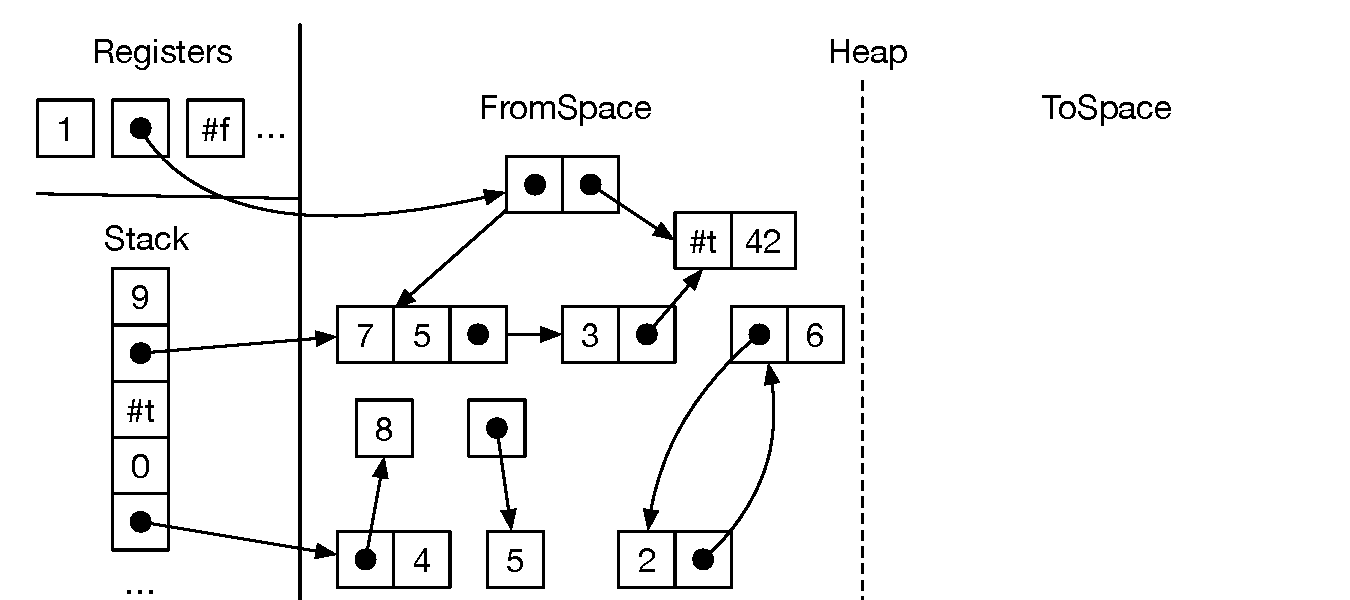
\includegraphics[width=\textwidth]{figs/copy-collect-1} \\[5ex]
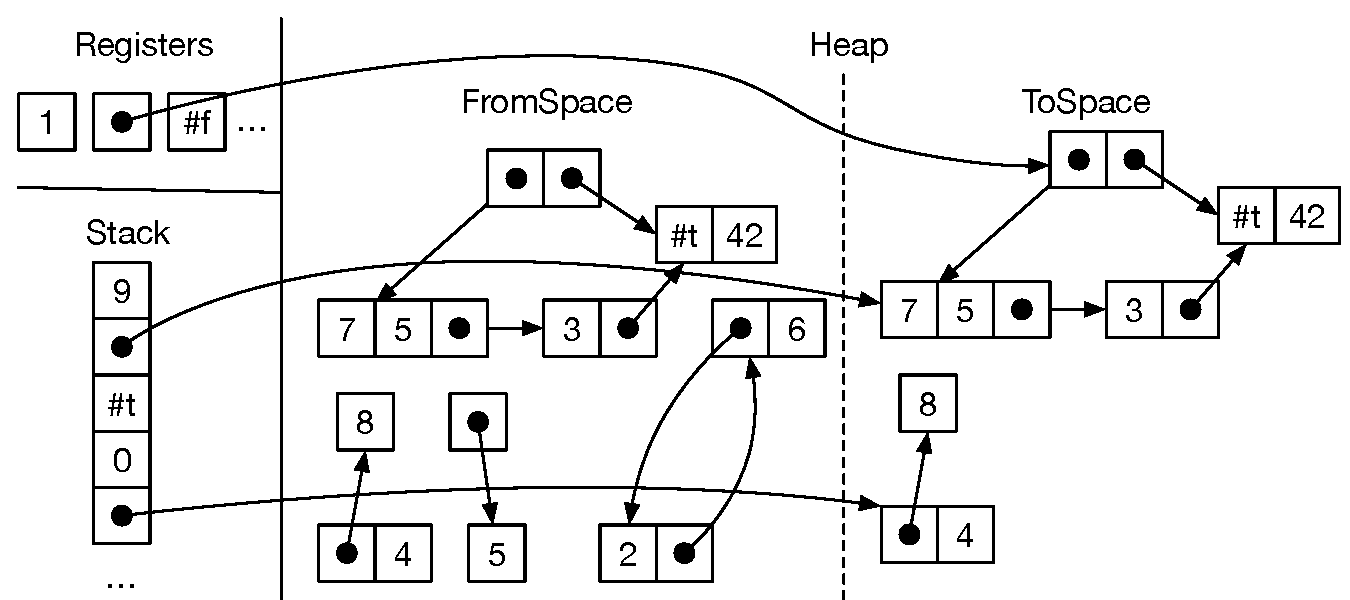
\includegraphics[width=\textwidth]{figs/copy-collect-2}
\caption{A copying collector in action.}
\label{fig:copying-collector}
\end{figure}

%% \margincomment{\tiny Need to add comment somewhere about the goodness
%%  of copying collection, especially that it doesn't touch
%%  the garbage, so its time complexity only depends on the
%%  amount of live data.\\ --Jeremy}

There are many alternatives to copying collectors (and their older
siblings, the generational collectors) when its comes to garbage
collection, such as mark-and-sweep and reference counting.  The
strengths of copying collectors are that allocation is fast (just a
test and pointer increment), there is no fragmentation, cyclic garbage
is collected, and the time complexity of collection only depends on
the amount of live data, and not on the amount of
garbage~\citep{Wilson:1992fk}. The main disadvantage of two-space
copying collectors is that they use a lot of space, though that
problem is ameliorated in generational collectors.  Racket and Scheme
programs tend to allocate many small objects and generate a lot of
garbage, so copying and generational collectors are a good fit.  Of
course, garbage collection is an active research topic, especially
concurrent garbage collection~\citep{Tene:2011kx}. Researchers are
continuously developing new techniques and revisiting old
trade-offs~\citep{Blackburn:2004aa,Jones:2011aa,Shahriyar:2013aa,Cutler:2015aa,Shidal:2015aa}.

\subsection{Graph Copying via Cheney's Algorithm}
\label{sec:cheney}

Let us take a closer look at how the copy works. The allocated objects
and pointers can be viewed as a graph and we need to copy the part of
the graph that is reachable from the root set. To make sure we copy
all of the reachable vertices in the graph, we need an exhaustive
graph traversal algorithm, such as depth-first search or breadth-first
search~\citep{Moore:1959aa,Cormen:2001uq}. Recall that such algorithms
take into account the possibility of cycles by marking which vertices
have already been visited, so as to ensure termination of the
algorithm. These search algorithms also use a data structure such as a
stack or queue as a to-do list to keep track of the vertices that need
to be visited. We shall use breadth-first search and a trick due to
\citet{Cheney:1970aa} for simultaneously representing the queue and
copying tuples into the ToSpace.

Figure~\ref{fig:cheney} shows several snapshots of the ToSpace as the
copy progresses. The queue is represented by a chunk of contiguous
memory at the beginning of the ToSpace, using two pointers to track
the front and the back of the queue. The algorithm starts by copying
all tuples that are immediately reachable from the root set into the
ToSpace to form the initial queue.  When we copy a tuple, we mark the
old tuple to indicate that it has been visited. (We discuss the
marking in Section~\ref{sec:data-rep-gc}.) Note that any pointers
inside the copied tuples in the queue still point back to the
FromSpace. Once the initial queue has been created, the algorithm
enters a loop in which it repeatedly processes the tuple at the front
of the queue and pops it off the queue.  To process a tuple, the
algorithm copies all the tuple that are directly reachable from it to
the ToSpace, placing them at the back of the queue. The algorithm then
updates the pointers in the popped tuple so they point to the newly
copied tuples. Getting back to Figure~\ref{fig:cheney}, in the first
step we copy the tuple whose second element is $42$ to the back of the
queue. The other pointer goes to a tuple that has already been copied,
so we do not need to copy it again, but we do need to update the
pointer to the new location. This can be accomplished by storing a
\emph{forwarding} pointer to the new location in the old tuple, back
when we initially copied the tuple into the ToSpace. This completes
one step of the algorithm. The algorithm continues in this way until
the front of the queue is empty, that is, until the front catches up
with the back.

\begin{figure}[tbp]
\centering 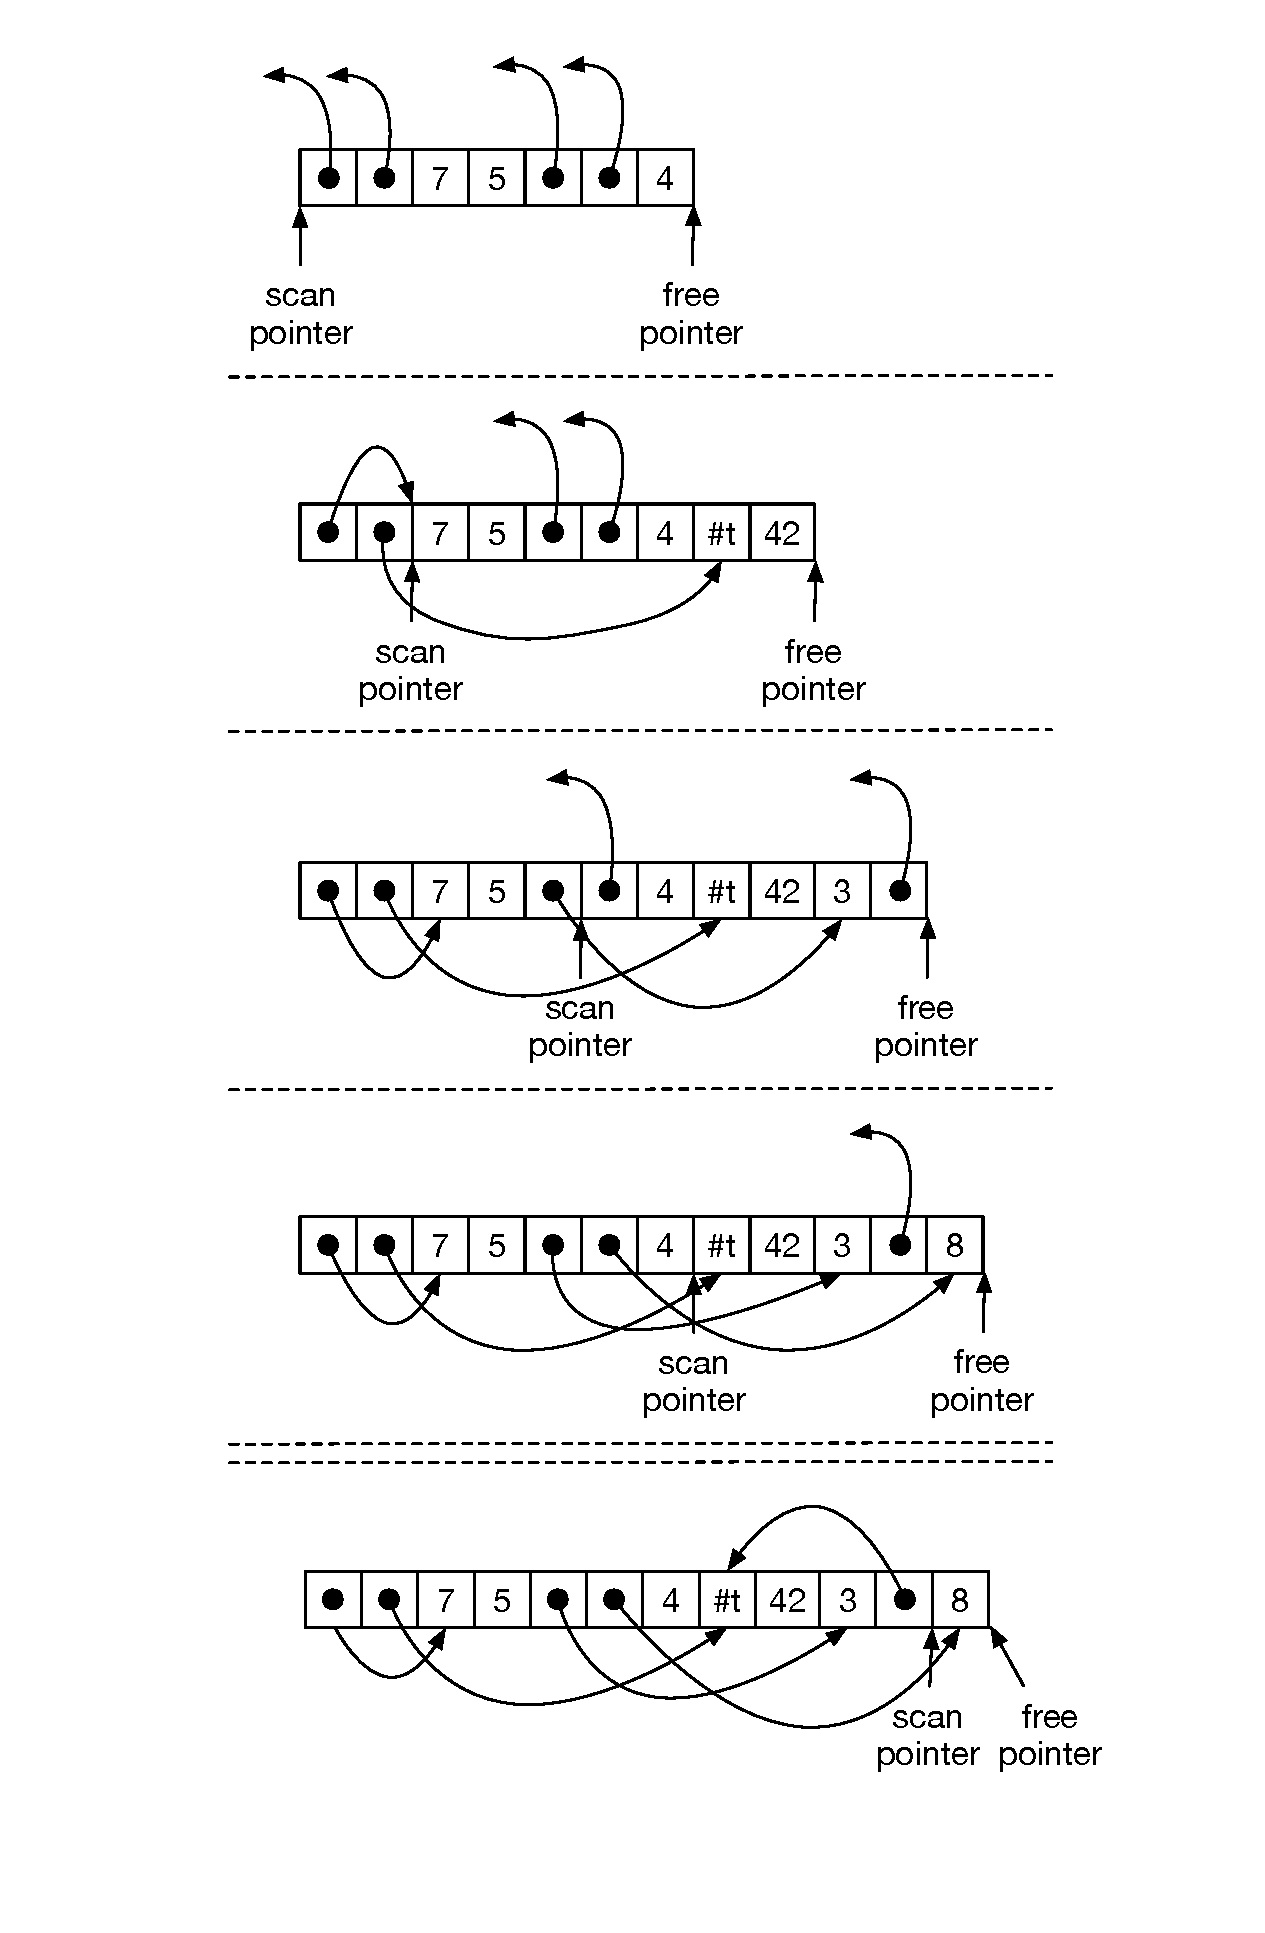
\includegraphics[width=0.9\textwidth]{figs/cheney}
\caption{Depiction of the Cheney algorithm copying the live tuples.}
\label{fig:cheney}
\end{figure}


\subsection{Data Representation}
\label{sec:data-rep-gc}

The garbage collector places some requirements on the data
representations used by our compiler. First, the garbage collector
needs to distinguish between pointers and other kinds of data. There
are several ways to accomplish this.
\begin{enumerate}
\item Attached a tag to each object that identifies what type of
  object it is~\citep{McCarthy:1960dz}.
\item Store different types of objects in different
  regions~\citep{Steele:1977ab}.
\item Use type information from the program to either generate
  type-specific code for collecting or to generate tables that can
  guide the
  collector~\citep{Appel:1989aa,Goldberg:1991aa,Diwan:1992aa}.
\end{enumerate}
Dynamically typed languages, such as Lisp, need to tag objects
anyways, so option 1 is a natural choice for those languages.
However, $R_3$ is a statically typed language, so it would be
unfortunate to require tags on every object, especially small and
pervasive objects like integers and Booleans.  Option 3 is the
best-performing choice for statically typed languages, but comes with
a relatively high implementation complexity. To keep this chapter to a
2-week time budget, we recommend a combination of options 1 and 2,
with separate strategies used for the stack and the heap.

Regarding the stack, we recommend using a separate stack for
pointers~\citep{Siebert:2001aa,Henderson:2002aa,Baker:2009aa}, which
we call a \emph{root stack} (a.k.a. ``shadow stack''). That is, when a
local variable needs to be spilled and is of type \code{(Vector
  $\Type_1 \ldots \Type_n$)}, then we put it on the root stack instead
of the normal procedure call stack. Furthermore, we always spill
vector-typed variables if they are live during a call to the
collector, thereby ensuring that no pointers are in registers during a
collection. Figure~\ref{fig:shadow-stack} reproduces the example from
Figure~\ref{fig:copying-collector} and contrasts it with the data
layout using a root stack. The root stack contains the two pointers
from the regular stack and also the pointer in the second
register.

\begin{figure}[tbp]
\centering 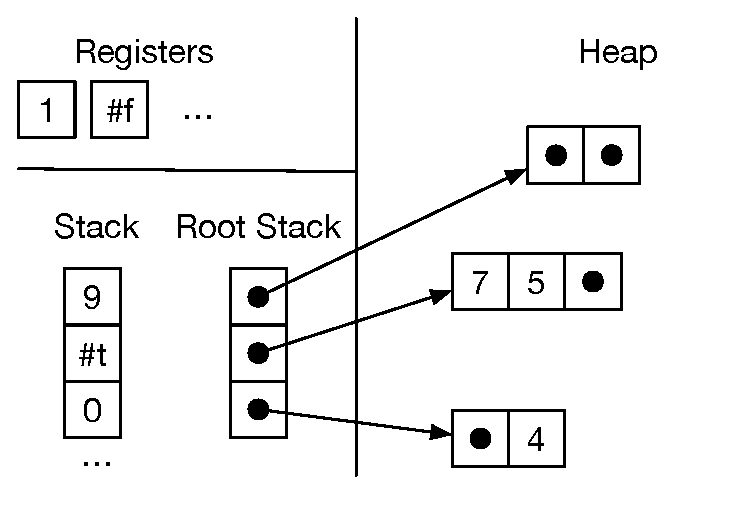
\includegraphics[width=0.7\textwidth]{figs/root-stack}
\caption{Maintaining a root stack to facilitate garbage collection.}
\label{fig:shadow-stack}
\end{figure}

The problem of distinguishing between pointers and other kinds of data
also arises inside of each tuple. We solve this problem by attaching a
tag, an extra 64-bits, to each tuple. Figure~\ref{fig:tuple-rep} zooms
in on the tags for two of the tuples in the example from
Figure~\ref{fig:copying-collector}. Part of each tag is dedicated to
specifying which elements of the tuple are pointers, the part labeled
``pointer mask''. Within the pointer mask, a 1 bit indicates there is
a pointer and a 0 bit indicates some other kind of data. The pointer
mask starts at bit location 7. We have limited tuples to a maximum
size of 50 elements, so we just need 50 bits for the pointer mask. The
tag also contains two other pieces of information. The length of the
tuple (number of elements) is stored in bits location 1 through
6. Finally, the bit at location 0 indicates whether the tuple has yet
to be copied to the FromSpace.  If the bit has value 1, then this
tuple has not yet been copied.  If the bit has value 0 then the entire
tag is in fact a forwarding pointer. (The lower 3 bits of an pointer
are always zero anyways because our tuples are 8-byte aligned.)

\begin{figure}[tbp]
\centering 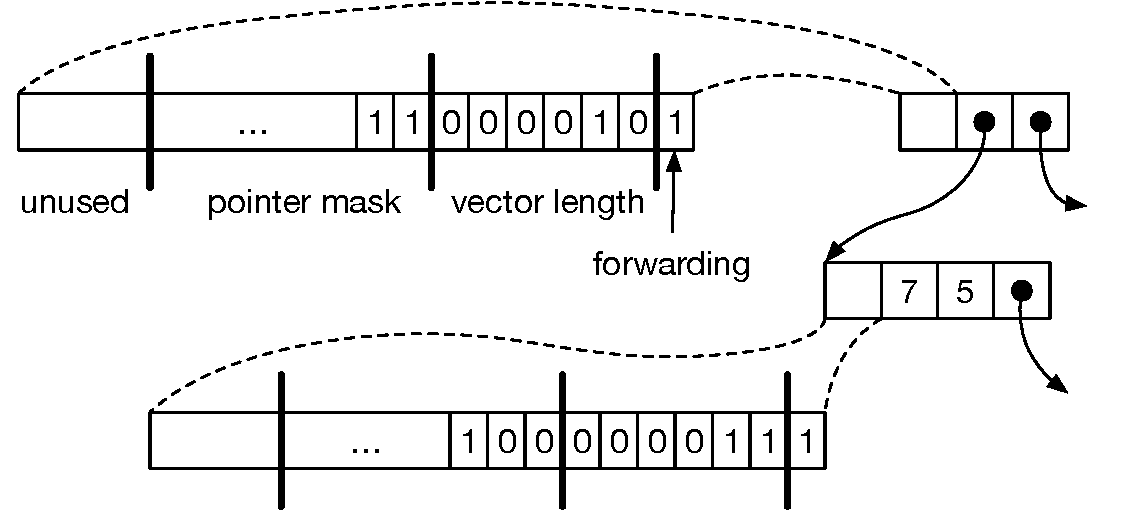
\includegraphics[width=0.8\textwidth]{figs/tuple-rep}
\caption{Representation for tuples in the heap.}
\label{fig:tuple-rep}
\end{figure}

\subsection{Implementation of the Garbage Collector}
\label{sec:organize-gz}

The implementation of the garbage collector needs to do a lot of
bit-level data manipulation and we need to link it with our
compiler-generated x86 code. Thus, we recommend implementing the
garbage collector in C~\citep{Kernighan:1988nx} and putting the code
in the \code{runtime.c} file. Figure~\ref{fig:gc-header} shows the
interface to the garbage collector. The \code{initialize} function
creates the FromSpace, ToSpace, and root stack. The \code{initialize}
function is meant to be called near the beginning of \code{main},
before the rest of the program executes.  The \code{initialize}
function puts the address of the beginning of the FromSpace into the
global variable \code{free\_ptr}. The global \code{fromspace\_end}
points to the address that is 1-past the last element of the
FromSpace. (We use half-open intervals to represent chunks of
memory~\citep{Dijkstra:1982aa}.)  The \code{rootstack\_begin} global
points to the first element of the root stack.

As long as there is room left in the FromSpace, your generated code
can allocate tuples simply by moving the \code{free\_ptr} forward.
%
\margincomment{\tiny Should we dedicate a register to the free pointer? \\
--Jeremy}
%
The amount of room left in FromSpace is the difference between the
\code{fromspace\_end} and the \code{free\_ptr}.  The \code{collect}
function should be called when there is not enough room left in the
FromSpace for the next allocation.  The \code{collect} function takes
a pointer to the current top of the root stack (one past the last item
that was pushed) and the number of bytes that need to be
allocated. The \code{collect} function performs the copying collection
and leaves the heap in a state such that the next allocation will
succeed.

\begin{figure}[tbp]
\begin{lstlisting}
   void initialize(uint64_t rootstack_size, uint64_t heap_size);
   void collect(int64_t** rootstack_ptr, uint64_t bytes_requested);
   int64_t* free_ptr;
   int64_t* fromspace_begin;
   int64_t* fromspace_end;
   int64_t** rootstack_begin;
\end{lstlisting}
\caption{The compiler's interface to the garbage collector.}
\label{fig:gc-header}
\end{figure}

\begin{exercise}
  In the file \code{runtime.c} you will find the implementation of
  \code{initialize} and a partial implementation of \code{collect}.
  The \code{collect} function calls another function, \code{cheney},
  to perform the actual copy, and that function is left to the reader
  to implement. The following is the prototype for \code{cheney}.
\begin{lstlisting}
   static void cheney(int64_t** rootstack_ptr);
\end{lstlisting}
  The parameter \code{rootstack\_ptr} is a pointer to the top of the
  rootstack (which is an array of pointers).  The \code{cheney} function
  also communicates with \code{collect} through several global
  variables, the \code{fromspace\_begin} and \code{fromspace\_end}
  mentioned in Figure~\ref{fig:gc-header} as well as the pointers for
  the ToSpace:
\begin{lstlisting}
   static int64_t* tospace_begin;
   static int64_t* tospace_end;
\end{lstlisting}
  The job of the \code{cheney} function is to copy all the live
  objects (reachable from the root stack) into the ToSpace, update
  \code{free\_ptr} to point to the next unused spot in the ToSpace,
  update the root stack so that it points to the objects in the
  ToSpace, and finally to swap the global pointers for the FromSpace
  and ToSpace.
\end{exercise}


\section{Compiler Passes}
\label{sec:code-generation-gc}

The introduction of garbage collection has a non-trivial impact on our
compiler passes. We introduce one new compiler pass called
\code{expose-allocation} and make non-trivial changes to
\code{type-check}, \code{flatten}, \code{select-instructions},
\code{allocate-registers}, and \code{print-x86}.  The following
program will serve as our running example.  It creates two tuples, one
nested inside the other. Both tuples have length one. The example then
accesses the element in the inner tuple tuple via two vector
references.
% tests/s2_17.rkt
\begin{lstlisting}
   (vector-ref (vector-ref (vector (vector 42)) 0) 0))
\end{lstlisting}

We already discuss the changes to \code{type-check} in
Section~\ref{sec:r3}, including the addition of \code{has-type}, so we
proceed to discuss the new \code{expose-allocation} pass.

\subsection{Expose Allocation (New)}
\label{sec:expose-allocation}

The pass \code{expose-allocation} lowers the \code{vector} creation
form into a conditional call to the collector followed by the
allocation. We choose to place the \code{expose-allocation} pass
before \code{flatten} because \code{expose-allocation} introduces new
variables, which can be done locally with \code{let}, but \code{let}
is gone after \code{flatten}.  In the following, we show the
transformation for the \code{vector} form into let-bindings for the
intializing expressions, by a conditional \code{collect}, an
\code{allocate}, and the initialization of the vector.
(The \itm{len} is the length of the vector and \itm{bytes} is how many
total bytes need to be allocated for the vector, which is 8 for the
tag plus \itm{len} times 8.)

\begin{lstlisting}
  (has-type (vector |$e_0 \ldots e_{n-1}$|) |\itm{type}|)
|$\Longrightarrow$|
  (let ([|$x_0$| |$e_0$|]) ... (let ([|$x_{n-1}$| |$e_{n-1}$|])
  (let ([_ (if (< (+ (global-value free_ptr) |\itm{bytes}|)
                  (global-value fromspace_end))
               (void)
               (collect |\itm{bytes}|))])
  (let ([|$v$| (allocate |\itm{len}| |\itm{type}|)])
  (let ([_ (vector-set! |$v$| |$0$| |$x_0$|)]) ...
  (let ([_ (vector-set! |$v$| |$n-1$| |$x_{n-1}$|)])
     |$v$|) ... )))) ...)
\end{lstlisting}
(In the above, we suppressed all of the \code{has-type} forms in the
output for the sake of readability.)  The ordering of the initializing
expressions ($e_0,\ldots,e_{n-1}$) prior to the \code{allocate} is
important, as those expressions may trigger garbage collection and we
do not want an allocated but uninitialized tuple to be present during
a garbage collection.

The output of \code{expose-allocation} is a language that extends
$R_3$ with the three new forms that we use above in the translation of
\code{vector}.
\[
\begin{array}{lcl}
  \Exp &::=& \cdots
      \mid (\key{collect} \,\itm{int})
      \mid (\key{allocate} \,\itm{int}\,\itm{type})
      \mid (\key{global-value} \,\itm{name})
\end{array}
\]

%% The \code{expose-allocation} inserts an \code{initialize} statement at
%% the beginning of the program which will instruct the garbage collector
%% to set up the FromSpace, ToSpace, and all the global variables.  The
%% two arguments of \code{initialize} specify the initial allocated space
%% for the root stack and for the heap.
%
%% The \code{expose-allocation} pass annotates all of the local variables
%% in the \code{program} form with their type.


Figure~\ref{fig:expose-alloc-output} shows the output of the
\code{expose-allocation} pass on our running example.

\begin{figure}[tbp]
\begin{lstlisting}
(program (type Integer)
 (vector-ref
  (vector-ref
   (let ((vecinit32990
	  (let ([vecinit32986 42])
	    (let ((collectret32988
		   (if (< (+ (global-value free_ptr) 16)
			  (global-value fromspace_end))
		       (void)
		       (collect 16))))
	      (let ([alloc32985
		     (allocate 1 (Vector Integer))])
		(let ([initret32987
		       (vector-set! alloc32985 0 vecinit32986)])
		  alloc32985))))))
     (let ([collectret32992
	    (if (< (+ (global-value free_ptr) 16)
                   (global-value fromspace_end))
                (void)
                (collect 16))])
       (let ([alloc32989 (allocate 1 (Vector (Vector Integer)))])
	 (let ([initret32991 (vector-set! alloc32989 0 vecinit32990)])
	   alloc32989))))
   0)
  0))
\end{lstlisting}
\caption{Output of the \code{expose-allocation} pass, minus
  all of the \code{has-type} forms.}
\label{fig:expose-alloc-output}
\end{figure}


\clearpage

\subsection{Flatten and the $C_2$ intermediate language}
\label{sec:flatten-gc}

\begin{figure}[tp]
\fbox{
\begin{minipage}{0.96\textwidth}
\[
\begin{array}{lcl}
\Arg &::=& \gray{ \Int \mid \Var \mid \key{\#t} \mid \key{\#f} }\\
\itm{cmp} &::= & \gray{  \key{eq?} \mid \key{<} \mid \key{<=} \mid \key{>} \mid \key{>=}  } \\
\Exp &::= & \gray{ \Arg \mid (\key{read}) \mid (\key{-}\;\Arg) \mid (\key{+} \; \Arg\;\Arg)
      \mid (\key{not}\;\Arg) \mid (\itm{cmp}\;\Arg\;\Arg)  } \\
   &\mid& (\key{allocate} \,\itm{int}\,\itm{type})
   \mid (\key{vector-ref}\, \Arg\, \Int)  \\
   &\mid& (\key{vector-set!}\,\Arg\,\Int\,\Arg)
    \mid (\key{global-value} \,\itm{name}) \mid (\key{void}) \\
\Stmt &::=& \gray{ \ASSIGN{\Var}{\Exp} \mid \RETURN{\Arg} } \\
      &\mid& \gray{ \IF{(\itm{cmp}\, \Arg\,\Arg)}{\Stmt^{*}}{\Stmt^{*}} } \\
      &\mid& (\key{collect} \,\itm{int}) \\
C_2 & ::= & \gray{ (\key{program}\;(\Var^{*})\;(\key{type}\;\textit{type})\;\Stmt^{+}) }
\end{array}
\]
\end{minipage}
}
\caption{The $C_2$ language, extending $C_1$ with support for tuples.}
\label{fig:c2-syntax}
\end{figure}

The output of \code{flatten} is a program in the intermediate language
$C_2$, whose syntax is defined in Figure~\ref{fig:c2-syntax}.  The new
forms of $C_2$ include the expressions \key{allocate},
\key{vector-ref}, and \key{vector-set!}, and \key{global-value} and
the statement \code{collect}.  The \code{flatten} pass can treat these
new forms much like the other forms.

Recall that the \code{flatten} function collects all of the local
variables so that it can decorate the \code{program} form with
them. Also recall that we need to know the types of all the local
variables for purposes of identifying the root set for the garbage
collector.  Thus, we change \code{flatten} to collect not just the
variables, but the variables and their types in the form of an
association list.  Thanks to the \code{has-type} forms, the types are
readily available.  For example, consider the translation of the
\code{let} form.
\begin{lstlisting}
  (let ([|$x$| (has-type |\itm{rhs}| |\itm{type}|)]) |\itm{body}|)
|$\Longrightarrow$|
  (values |\itm{body'}|
          (|\itm{ss_1}| (assign |$x$| |\itm{rhs'}|)  |\itm{ss_2}|)
          ((|$x$| . |\itm{type}|) |\itm{xt_1}| |\itm{xt_2}|))
\end{lstlisting}
where \itm{rhs'}, \itm{ss_1}, and \itm{xs_1} are the results of
recursively flattening \itm{rhs} and \itm{body'}, \itm{ss_2}, and
\itm{xs_2} are the results of recursively flattening \itm{body}.  The
output on our running example is shown in Figure~\ref{fig:flatten-gc}.

\begin{figure}[tbp]
\begin{lstlisting}
'(program
  ((tmp02 . Integer) (tmp01 Vector Integer) (tmp90 Vector Integer)
   (tmp86 . Integer) (tmp88 . Void) (tmp96 . Void)
   (tmp94 . Integer) (tmp93 . Integer) (tmp95 . Integer)
   (tmp85 Vector Integer) (tmp87 . Void) (tmp92 . Void)
   (tmp00 . Void) (tmp98 . Integer) (tmp97 . Integer)
   (tmp99 . Integer) (tmp89 Vector (Vector Integer))
   (tmp91 . Void))
  (type Integer)
  (assign tmp86 42)
  (assign tmp93 (global-value free_ptr))
  (assign tmp94 (+ tmp93 16))
  (assign tmp95 (global-value fromspace_end))
  (if (< tmp94 tmp95)
    ((assign tmp96 (void)))
    ((collect 16) (assign tmp96 (void))))
  (assign tmp88 tmp96)
  (assign tmp85 (allocate 1 (Vector Integer)))
  (assign tmp87 (vector-set! tmp85 0 tmp86))
  (assign tmp90 tmp85)
  (assign tmp97 (global-value free_ptr))
  (assign tmp98 (+ tmp97 16))
  (assign tmp99 (global-value fromspace_end))
  (if (< tmp98 tmp99)
    ((assign tmp00 (void)))
    ((collect 16) (assign tmp00 (void))))
  (assign tmp92 tmp00)
  (assign tmp89 (allocate 1 (Vector (Vector Integer))))
  (assign tmp91 (vector-set! tmp89 0 tmp90))
  (assign tmp01 (vector-ref tmp89 0))
  (assign tmp02 (vector-ref tmp01 0))
  (return tmp02))
\end{lstlisting}
\caption{Output of \code{flatten} for the running example.}
\label{fig:flatten-gc}
\end{figure}

\clearpage

\subsection{Select Instructions}
\label{sec:select-instructions-gc}

%% void (rep as zero)
%% allocate
%% collect (callq collect)
%% vector-ref
%% vector-set!
%% global-value (postpone)

In this pass we generate x86 code for most of the new operations that
were needed to compile tuples, including \code{allocate},
\code{collect}, \code{vector-ref}, \code{vector-set!}, and
\code{(void)}. We postpone \code{global-value} to \code{print-x86}.

The \code{vector-ref} and \code{vector-set!} forms translate into
\code{movq} instructions with the appropriate \key{deref}.  (The
plus one is to get past the tag at the beginning of the tuple
representation.)
\begin{lstlisting}
   (assign |$\itm{lhs}$| (vector-ref |$\itm{vec}$| |$n$|))
   |$\Longrightarrow$|
   (movq |$\itm{vec}'$| (reg r11))
   (movq (deref r11 |$8(n+1)$|) |$\itm{lhs}$|)

   (assign |$\itm{lhs}$| (vector-set! |$\itm{vec}$| |$n$| |$\itm{arg}$|))
   |$\Longrightarrow$|
   (movq |$\itm{vec}'$| (reg r11))
   (movq |$\itm{arg}'$| (deref r11 |$8(n+1)$|))
   (movq (int 0) |$\itm{lhs}$|)
\end{lstlisting}
The $\itm{vec}'$ and $\itm{arg}'$ are obtained by recursively
processing $\itm{vec}$ and $\itm{arg}$.  The move of $\itm{vec}'$ to
register \code{r11} ensures that offsets are only performed with
register operands. This requires removing \code{r11} from
consideration by the register allocating.

We compile the \code{allocate} form to operations on the
\code{free\_ptr}, as shown below. The address in the \code{free\_ptr}
is the next free address in the FromSpace, so we move it into the
\itm{lhs} and then move it forward by enough space for the tuple being
allocated, which is $8(\itm{len}+1)$ bytes because each element is 8
bytes (64 bits) and we use 8 bytes for the tag. Last but not least, we
initialize the \itm{tag}. Refer to Figure~\ref{fig:tuple-rep} to see
how the tag is organized. We recommend using the Racket operations
\code{bitwise-ior} and \code{arithmetic-shift} to compute the tag.
The type annoation in the \code{vector} form is used to determine the
pointer mask region of the tag.
\begin{lstlisting}
   (assign |$\itm{lhs}$| (allocate |$\itm{len}$| (Vector |$\itm{type} \ldots$|)))
   |$\Longrightarrow$|
   (movq (global-value free_ptr) |$\itm{lhs}'$|)
   (addq (int |$8(\itm{len}+1)$|) (global-value free_ptr))
   (movq |$\itm{lhs}'$| (reg r11))
   (movq (int |$\itm{tag}$|) (deref r11 0))
\end{lstlisting}

The \code{collect} form is compiled to a call to the \code{collect}
function in the runtime. The arguments to \code{collect} are the top
of the root stack and the number of bytes that need to be allocated.
We shall use a dedicated register, \code{r15}, to store the pointer to
the top of the root stack. So \code{r15} is not available for use by
the register allocator.
\begin{lstlisting}
   (collect |$\itm{bytes}$|)
   |$\Longrightarrow$|
   (movq (reg 15) (reg rdi))
   (movq |\itm{bytes}| (reg rsi))
   (callq collect)
\end{lstlisting}


\begin{figure}[tp]
\fbox{
\begin{minipage}{0.96\textwidth}
\[
\begin{array}{lcl}
\Arg &::=&  \gray{  \INT{\Int} \mid \REG{\itm{register}}
    \mid (\key{deref}\,\itm{register}\,\Int) } \\
   &\mid& \gray{ (\key{byte-reg}\; \itm{register})  }
   \mid (\key{global-value}\; \itm{name}) \\
\itm{cc} & ::= & \gray{  \key{e} \mid \key{l} \mid \key{le} \mid \key{g} \mid \key{ge}  } \\
\Instr &::=& \gray{(\key{addq} \; \Arg\; \Arg) \mid
             (\key{subq} \; \Arg\; \Arg) \mid
             (\key{negq} \; \Arg) \mid (\key{movq} \; \Arg\; \Arg)} \\
      &\mid& \gray{(\key{callq} \; \mathit{label}) \mid
             (\key{pushq}\;\Arg) \mid
             (\key{popq}\;\Arg) \mid
             (\key{retq})} \\
       &\mid& \gray{  (\key{xorq} \; \Arg\;\Arg)
       \mid (\key{cmpq} \; \Arg\; \Arg) \mid (\key{set}\itm{cc} \; \Arg)  } \\
       &\mid& \gray{  (\key{movzbq}\;\Arg\;\Arg)
       \mid  (\key{jmp} \; \itm{label})
       \mid (\key{j}\itm{cc} \; \itm{label})
       \mid (\key{label} \; \itm{label})  } \\
x86_2 &::= & \gray{  (\key{program} \;\itm{info} \;(\key{type}\;\itm{type})\; \Instr^{+})  }
\end{array}
\]
\end{minipage}
}
\caption{The x86$_2$ language (extends x86$_1$ of Figure~\ref{fig:x86-1}).}
\label{fig:x86-2}
\end{figure}

The syntax of the $x86_2$ language is defined in
Figure~\ref{fig:x86-2}.  It differs from $x86_1$ just in the addition
of the form for global variables.
%
Figure~\ref{fig:select-instr-output-gc} shows the output of the
\code{select-instructions} pass on the running example.

\begin{figure}[tbp]
\centering
\begin{minipage}{0.75\textwidth}
\begin{lstlisting}[basicstyle=\ttfamily\footnotesize]
(program
  ((tmp02 . Integer) (tmp01 Vector Integer) (tmp90 Vector Integer)
   (tmp86 . Integer) (tmp88 . Void) (tmp96 . Void) (tmp94 . Integer)
   (tmp93 . Integer) (tmp95 . Integer) (tmp85 Vector Integer)
   (tmp87 . Void) (tmp92 . Void) (tmp00 . Void) (tmp98 . Integer)
   (tmp97 . Integer) (tmp99 . Integer) (tmp89 Vector (Vector Integer))
   (tmp91 . Void)) (type Integer)
  (movq (int 42) (var tmp86))
  (movq (global-value free_ptr) (var tmp93))
  (movq (var tmp93) (var tmp94))
  (addq (int 16) (var tmp94))
  (movq (global-value fromspace_end) (var tmp95))
  (if (< (var tmp94) (var tmp95))
    ((movq (int 0) (var tmp96)))
    ((movq (reg r15) (reg rdi))
     (movq (int 16) (reg rsi))
     (callq collect)
     (movq (int 0) (var tmp96))))
  (movq (var tmp96) (var tmp88))
  (movq (global-value free_ptr) (var tmp85))
  (addq (int 16) (global-value free_ptr))
  (movq (var tmp85) (reg r11))
  (movq (int 3) (deref r11 0))
  (movq (var tmp85) (reg r11))
  (movq (var tmp86) (deref r11 8))
  (movq (int 0) (var tmp87))
  (movq (var tmp85) (var tmp90))
  (movq (global-value free_ptr) (var tmp97))
  (movq (var tmp97) (var tmp98))
  (addq (int 16) (var tmp98))
  (movq (global-value fromspace_end) (var tmp99))
  (if (< (var tmp98) (var tmp99))
    ((movq (int 0) (var tmp00)))
    ((movq (reg r15) (reg rdi))
     (movq (int 16) (reg rsi))
     (callq collect)
     (movq (int 0) (var tmp00))))
  (movq (var tmp00) (var tmp92))
  (movq (global-value free_ptr) (var tmp89))
  (addq (int 16) (global-value free_ptr))
  (movq (var tmp89) (reg r11))
  (movq (int 131) (deref r11 0))
  (movq (var tmp89) (reg r11))
  (movq (var tmp90) (deref r11 8))
  (movq (int 0) (var tmp91))
  (movq (var tmp89) (reg r11))
  (movq (deref r11 8) (var tmp01))
  (movq (var tmp01) (reg r11))
  (movq (deref r11 8) (var tmp02))
  (movq (var tmp02) (reg rax)))
\end{lstlisting}
\end{minipage}
\caption{Output of the \code{select-instructions} pass.}
\label{fig:select-instr-output-gc}
\end{figure}

\clearpage

\subsection{Register Allocation}
\label{sec:reg-alloc-gc}

As discussed earlier in this chapter, the garbage collector needs to
access all the pointers in the root set, that is, all variables that
are vectors. It will be the responsibility of the register allocator
to make sure that:
\begin{enumerate}
\item the root stack is used for spilling vector-typed variables, and
\item if a vector-typed variable is live during a call to the
  collector, it must be spilled to ensure it is visible to the
  collector.
\end{enumerate}

The later responsibility can be handled during construction of the
inference graph, by adding interference edges between the call-live
vector-typed variables and all the callee-save registers. (They
already interfere with the caller-save registers.)  The type
information for variables is in the \code{program} form, so we
recommend adding another parameter to the \code{build-interference}
function to communicate this association list.

The spilling of vector-typed variables to the root stack can be
handled after graph coloring, when choosing how to assign the colors
(integers) to registers and stack locations. The \code{program} output
of this pass changes to also record the number of spills to the root
stack.
\[
\begin{array}{lcl}
x86_2 &::= & (\key{program} \;(\itm{stackSpills} \; \itm{rootstackSpills}) \;(\key{type}\;\itm{type})\; \Instr^{+})
\end{array}
\]


% build-interference
%
% callq
%   extra parameter for var->type assoc. list
% update 'program' and 'if'

% allocate-registers
%    allocate spilled vectors to the rootstack

% don't change color-graph



\subsection{Print x86}
\label{sec:print-x86-gc}


\margincomment{\scriptsize We need to show the translation to x86 and what
  to do about global-value. \\ --Jeremy}

Figure~\ref{fig:print-x86-output-gc} shows the output of the
\code{print-x86} pass on the running example. In the prelude and
conclusion of the \code{main} function, we treat the root stack very
much like the regular stack in that we move the root stack pointer
(\code{r15}) to make room for all of the spills to the root stack,
except that the root stack grows up instead of down.  For the running
example, there was just one spill so we increment \code{r15} by 8
bytes. In the conclusion we decrement \code{r15} by 8 bytes.

One issue that deserves special care is that there may be a call to
\code{collect} prior to the initializing assignments for all the
variables in the root stack. We do not want the garbage collector to
accidentaly think that some uninitialized variable is a pointer that
needs to be followed. Thus, we zero-out all locations on the root
stack in the prelude of \code{main}. In
Figure~\ref{fig:print-x86-output-gc}, the instruction
%
\lstinline{movq $0, (%r15)} 
%
accomplishes this task. The garbage collector tests each root to see
if it is null prior to dereferencing it.

\begin{figure}[htbp]
\begin{minipage}[t]{0.5\textwidth}
\begin{lstlisting}[basicstyle=\ttfamily\scriptsize]
	.globl _main
_main:
	pushq	%rbp
	movq	%rsp, %rbp
	pushq	%r14
	pushq	%r13
	pushq	%r12
	pushq	%rbx
	subq	$0, %rsp
	movq $16384, %rdi
	movq $16, %rsi
	callq _initialize
	movq _rootstack_begin(%rip), %r15
	movq $0, (%r15)
	addq $8, %r15

	movq	$42, %rbx
	movq	_free_ptr(%rip), %rcx
	addq	$16, %rcx
	movq	_fromspace_end(%rip), %rdx
	cmpq	%rdx, %rcx
	jl then33131
	movq	%r15, %rdi
	movq	$16, %rsi
	callq	_collect
	movq	$0, %rcx
	jmp if_end33132
then33131:
	movq	$0, %rcx
if_end33132:
	movq	_free_ptr(%rip), %rcx
	addq	$16, _free_ptr(%rip)
	movq	%rcx, %r11
	movq	$3, 0(%r11)
	movq	%rcx, %r11
	movq	%rbx, 8(%r11)
	movq	$0, %rbx
	movq	%rcx, -8(%r15)
	movq	_free_ptr(%rip), %rbx
	movq	%rbx, %rcx
	addq	$16, %rcx
	movq	_fromspace_end(%rip), %rbx
	cmpq	%rbx, %rcx
	jl then33133
	movq	%r15, %rdi
	movq	$16, %rsi
	callq	_collect
	movq	$0, %rbx
	jmp if_end33134
\end{lstlisting}
\end{minipage}
\begin{minipage}[t]{0.45\textwidth}
\begin{lstlisting}[basicstyle=\ttfamily\scriptsize]
then33133:
	movq	$0, %rbx
if_end33134:
	movq	_free_ptr(%rip), %rbx
	addq	$16, _free_ptr(%rip)
	movq	%rbx, %r11
	movq	$131, 0(%r11)
	movq	%rbx, %r11
	movq	-8(%r15), %rax
	movq	%rax, 8(%r11)
	movq	$0, %rcx
	movq	%rbx, %r11
	movq	8(%r11), %rbx
	movq	%rbx, %r11
	movq	8(%r11), %rbx
	movq	%rbx, %rax

	movq	%rax, %rdi
	callq	_print_int
	movq	$0, %rax
	subq $8, %r15
	addq	$0, %rsp
	popq	%rbx
	popq	%r12
	popq	%r13
	popq	%r14
	popq	%rbp
	retq
\end{lstlisting}
\end{minipage}
\caption{Output of the \code{print-x86} pass.}
\label{fig:print-x86-output-gc}
\end{figure}


\margincomment{\scriptsize Suggest an implementation strategy
  in which the students first do the code gen and test that
  without GC (just use a big heap), then after that is debugged,
  implement the GC. \\ --Jeremy}


\begin{figure}[p]
\begin{tikzpicture}[baseline=(current  bounding  box.center)]
\node (R1) at (0,2)  {\large $R_1$};
\node (R1-2) at (3,2)  {\large $R_1$};
\node (R1-3) at (6,2)  {\large $R_1$};
\node (C1-1) at (6,0)  {\large $C_1$};
\node (C1-3) at (3,0)  {\large $C_1$};

\node (x86-2) at (3,-2)  {\large $\text{x86}^{*}$};
\node (x86-3) at (6,-2)  {\large $\text{x86}^{*}$};
\node (x86-4) at (9,-2) {\large $\text{x86}^{*}$};
\node (x86-5) at (12,-2) {\large $\text{x86}$};
\node (x86-6) at (12,-4) {\large $\text{x86}^{\dagger}$};

\node (x86-2-1) at (3,-4)  {\large $\text{x86}^{*}$};
\node (x86-2-2) at (6,-4)  {\large $\text{x86}^{*}$};

\path[->,bend left=15] (R1) edge [above] node {\ttfamily\footnotesize\color{red} typecheck} (R1-2);
\path[->,bend left=15] (R1-2) edge [above] node {\ttfamily\footnotesize uniquify} (R1-3);
\path[->,bend left=15] (R1-3) edge [right] node {\ttfamily\footnotesize\color{red} flatten} (C1-1);
\path[->,bend right=15] (C1-1) edge [above] node {\ttfamily\footnotesize\color{red} expose-alloc.} (C1-3);
\path[->,bend right=15] (C1-3) edge [left] node {\ttfamily\footnotesize\color{red} select-instr.} (x86-2);
\path[->,bend left=15] (x86-2) edge [right] node {\ttfamily\footnotesize uncover-live} (x86-2-1);
\path[->,bend right=15] (x86-2-1) edge [below] node {\ttfamily\footnotesize \color{red}build-inter.} (x86-2-2);
\path[->,bend right=15] (x86-2-2) edge [right] node {\ttfamily\footnotesize\color{red} allocate-reg.} (x86-3);
\path[->,bend left=15] (x86-3) edge [above] node {\ttfamily\footnotesize lower-cond.} (x86-4);
\path[->,bend left=15] (x86-4) edge [above] node {\ttfamily\footnotesize patch-instr.} (x86-5);
\path[->,bend right=15] (x86-5) edge [left] node {\ttfamily\footnotesize\color{red} print-x86} (x86-6);
\end{tikzpicture}
\caption{Diagram of the passes for $R_3$, a language with tuples.}
\label{fig:R3-passes}
\end{figure}

Figure~\ref{fig:R3-passes} gives an overview of all the passes needed
for the compilation of $R_3$.


%%%%%%%%%%%%%%%%%%%%%%%%%%%%%%%%%%%%%%%%%%%%%%%%%%%%%%%%%%%%%%%%%%%%%%%%%%%%%%%%
\chapter{Functions}
\label{ch:functions}

This chapter studies the compilation of functions (aka. procedures) at
the level of abstraction of the C language. This corresponds to a
subset of Typed Racket in which only top-level function definitions
are allowed. This abstraction level is an important stepping stone to
implementing lexically-scoped functions in the form of \key{lambda}
abstractions (Chapter~\ref{ch:lambdas}).

\section{The $R_4$ Language}

The syntax for function definitions and function application
(aka. function call) is shown in Figure~\ref{fig:r4-syntax}, where we
define the $R_4$ language.  Programs in $R_4$ start with zero or more
function definitions.  The function names from these definitions are
in-scope for the entire program, including all other function
definitions (so the ordering of function definitions does not matter).

Functions are first-class in the sense that a function pointer is data
and can be stored in memory or passed as a parameter to another
function.  Thus, we introduce a function type, written
\begin{lstlisting}
   (|$\Type_1$| |$\cdots$| |$\Type_n$| -> |$\Type_r$|)
\end{lstlisting}
for a function whose $n$ parameters have the types $\Type_1$ through
$\Type_n$ and whose return type is $\Type_r$. The main limitation of
these functions (with respect to Racket functions) is that they are
not lexically scoped. That is, the only external entities that can be
referenced from inside a function body are other globally-defined
functions. The syntax of $R_4$ prevents functions from being nested
inside each other; they can only be defined at the top level.

\begin{figure}[tp]
\centering
\fbox{
\begin{minipage}{0.96\textwidth}
\[
\begin{array}{lcl}
  \Type &::=& \gray{ \key{Integer} \mid \key{Boolean}
         \mid (\key{Vector}\;\Type^{+}) \mid \key{Void}  } \mid (\Type^{*} \; \key{->}\; \Type) \\
\itm{cmp} &::= & \gray{  \key{eq?} \mid \key{<} \mid \key{<=} \mid \key{>} \mid \key{>=}  } \\
  \Exp &::=& \gray{ \Int \mid (\key{read}) \mid (\key{-}\;\Exp) \mid (\key{+} \; \Exp\;\Exp)}  \\
     &\mid&  \gray{ \Var \mid \LET{\Var}{\Exp}{\Exp} }\\
    &\mid& \gray{ \key{\#t} \mid \key{\#f} \mid
      (\key{and}\;\Exp\;\Exp) \mid (\key{not}\;\Exp)} \\
      &\mid& \gray{(\itm{cmp}\;\Exp\;\Exp) \mid \IF{\Exp}{\Exp}{\Exp}} \\
  &\mid& \gray{(\key{vector}\;\Exp^{+}) \mid
    (\key{vector-ref}\;\Exp\;\Int)} \\
  &\mid& \gray{(\key{vector-set!}\;\Exp\;\Int\;\Exp)\mid (\key{void})} \\
      &\mid& (\Exp \; \Exp^{*}) \\
  \Def &::=& (\key{define}\; (\Var \; [\Var \key{:} \Type]^{*}) \key{:} \Type \; \Exp) \\
  R_4 &::=& (\key{program} \; \Def^{*} \; \Exp)
\end{array}
\]
\end{minipage}
}
\caption{Syntax of $R_4$, extending $R_3$ with functions.}
\label{fig:r4-syntax}
\end{figure}

The program in Figure~\ref{fig:r4-function-example} is a
representative example of defining and using functions in $R_4$.  We
define a function \code{map-vec} that applies some other function
\code{f} to both elements of a vector (a 2-tuple) and returns a new
vector containing the results. We also define a function \code{add1}
that does what its name suggests. The program then applies
\code{map-vec} to \code{add1} and \code{(vector 0 41)}.  The result is
\code{(vector 1 42)}, from which we return the \code{42}.

\begin{figure}[tbp]
\begin{lstlisting}
(program
  (define (map-vec [f : (Integer -> Integer)]
                     [v : (Vector Integer Integer)])
          : (Vector Integer Integer)
    (vector (f (vector-ref v 0)) (f (vector-ref v 1))))
  (define (add1 [x : Integer]) : Integer
    (+ x 1))
  (vector-ref (map-vec add1 (vector 0 41)) 1)
  )
\end{lstlisting}
\caption{Example of using functions in $R_4$.}
\label{fig:r4-function-example}
\end{figure}

The definitional interpreter for $R_4$ is in
Figure~\ref{fig:interp-R4}.


\begin{figure}[tp]
\begin{lstlisting}
   (define (interp-R4 env)
     (lambda (e)
       (match e
          ....
          [`(define (,f [,xs : ,ps] ...) : ,rt ,body)
           (cons f `(lambda ,xs ,body))]
          [`(program ,ds ... ,body)
           (let ([top-level (map  (interp-R4 '()) ds)])
	      ((interp-R4 top-level) body))]
          [`(,fun ,args ...)
	    (define arg-vals (map (interp-R4 env) args))
            (define fun-val ((interp-R4 env) fun))
            (match fun-val
               [`(lambda (,xs ...) ,body)
                 (define new-env (append (map cons xs arg-vals) env))
 		 ((interp-R4 new-env) body)]
               [else (error "interp-R4, expected function, not" fun-val)]))]
         [else (error 'interp-R4 "unrecognized expression")]
         )))
\end{lstlisting}
\caption{Interpreter for the $R_4$ language.}
\label{fig:interp-R4}
\end{figure}


\section{Functions in x86}
\label{sec:fun-x86}

\margincomment{\tiny Make sure callee save registers are discussed
   in enough depth, especially updating Fig 6.4 \\ --Jeremy }

\margincomment{\tiny Talk about the return address on the
   stack and what callq  and retq does.\\ --Jeremy }

The x86 architecture provides a few features to support the
implementation of functions. We have already seen that x86 provides
labels so that one can refer to the location of an instruction, as is
needed for jump instructions. Labels can also be used to mark the
beginning of the instructions for a function.  Going further, we can
obtain the address of a label by using the \key{leaq} instruction and
\key{rip}-relative addressing. For example, the following puts the
address of the \code{add1} label into the \code{rbx} register.
\begin{lstlisting}
   leaq add1(%rip), %rbx
\end{lstlisting}

In Sections~\ref{sec:x86} and \ref{sec:select-s0} we saw the use of
the \code{callq} instruction for jumping to a function as specified by
a label. The use of the instruction changes slightly if the function
is specified by an address in a register, that is, an \emph{indirect
  function call}. The x86 syntax is to give the register name prefixed
with an asterisk.
\begin{lstlisting}
   callq *%rbx
\end{lstlisting}

The x86 architecture does not directly support passing arguments to
functions; instead we use a combination of registers and stack
locations for passing arguments, following the conventions used by
\code{gcc} as described by \cite{Matz:2013aa}. Up to six arguments may
be passed in registers, using the registers \code{rdi}, \code{rsi},
\code{rdx}, \code{rcx}, \code{r8}, and \code{r9}, in that order.  If
there are more than six arguments, then the rest must be placed on the
stack, which we call \emph{stack arguments}, which we discuss in later
paragraphs. The register \code{rax} is for the return value of the
function.

Recall from Section~\ref{sec:x86} that the stack is also used for
local variables and for storing the values of callee-save registers
(we shall refer to all of these collectively as ``locals''), and that
at the beginning of a function we move the stack pointer \code{rsp}
down to make room for them.
%% We recommend storing the local variables
%% first and then the callee-save registers, so that the local variables
%% can be accessed using \code{rbp} the same as before the addition of
%% functions.
To make additional room for passing arguments, we shall
move the stack pointer even further down. We count how many stack
arguments are needed for each function call that occurs inside the
body of the function and find their maximum. Adding this number to the
number of locals gives us how much the \code{rsp} should be moved at
the beginning of the function. In preparation for a function call, we
offset from \code{rsp} to set up the stack arguments. We put the first
stack argument in \code{0(\%rsp)}, the second in \code{8(\%rsp)}, and
so on.

Upon calling the function, the stack arguments are retrieved by the
callee using the base pointer \code{rbp}. The address \code{16(\%rbp)}
is the location of the first stack argument, \code{24(\%rbp)} is the
address of the second, and so on. Figure~\ref{fig:call-frames} shows
the layout of the caller and callee frames. Notice how important it is
that we correctly compute the maximum number of arguments needed for
function calls; if that number is too small then the arguments and
local variables will smash into each other!

As discussed in Section~\ref{sec:print-x86-reg-alloc}, an x86 function
is responsible for following conventions regarding the use of
registers: the caller should assume that all the caller save registers
get overwritten with arbitrary values by the callee. Thus, the caller
should either 1) not put values that are live across a call in caller
save registers, or 2) save and restore values that are live across
calls. We shall recommend option 1).  On the flip side, if the callee
wants to use a callee save register, the callee must arrange to put
the original value back in the register prior to returning to the
caller.


\begin{figure}[tbp]
\centering
\begin{tabular}{r|r|l|l} \hline
Caller View & Callee View & Contents       & Frame \\ \hline
8(\key{\%rbp})  & & return address & \multirow{5}{*}{Caller}\\
0(\key{\%rbp})  &  & old \key{rbp} \\
-8(\key{\%rbp}) &  & local $1$ \\
\ldots & & \ldots \\
$-8k$(\key{\%rbp}) &  & local $k$ \\
 & &  \\
$8n-8$\key{(\%rsp)} & $8n+8$(\key{\%rbp})& argument $n$ \\
& \ldots           & \ldots \\
0\key{(\%rsp)} & 16(\key{\%rbp})  & argument $1$   & \\ \hline
& 8(\key{\%rbp})   & return address & \multirow{5}{*}{Callee}\\
& 0(\key{\%rbp})   & old \key{rbp} \\
& -8(\key{\%rbp})  & local $1$ \\
&  \ldots          & \ldots \\
& $-8m$(\key{\%rsp})   & local $m$\\ \hline
\end{tabular}

\caption{Memory layout of caller and callee frames.}
\label{fig:call-frames}
\end{figure}


\section{The compilation of functions}

\margincomment{\scriptsize To do: discuss the need to push and
  pop call-live pointers (vectors and functions)
  to the root stack \\ --Jeremy}

Now that we have a good understanding of functions as they appear in
$R_4$ and the support for functions in x86, we need to plan the
changes to our compiler, that is, do we need any new passes and/or do
we need to change any existing passes? Also, do we need to add new
kinds of AST nodes to any of the intermediate languages?

\begin{figure}[tp]
\centering
\fbox{
\begin{minipage}{0.96\textwidth}
\[
\begin{array}{lcl}
  \Type &::=& \gray{ \key{Integer} \mid \key{Boolean}
         \mid (\key{Vector}\;\Type^{+}) \mid \key{Void}  } \mid (\Type^{*} \; \key{->}\; \Type) \\
  \Exp &::=& \gray{ \Int \mid (\key{read}) \mid (\key{-}\;\Exp) \mid (\key{+} \; \Exp\;\Exp)}  \\
     &\mid&  (\key{function-ref}\, \itm{label})
     \mid \gray{ \Var \mid \LET{\Var}{\Exp}{\Exp} }\\
  &\mid& \gray{ \key{\#t} \mid \key{\#f} \mid
      (\key{and}\;\Exp\;\Exp) \mid (\key{not}\;\Exp)} \\
      &\mid& \gray{(\itm{cmp}\;\Exp\;\Exp) \mid \IF{\Exp}{\Exp}{\Exp}} \\
  &\mid& \gray{(\key{vector}\;\Exp^{+}) \mid
    (\key{vector-ref}\;\Exp\;\Int)} \\
  &\mid& \gray{(\key{vector-set!}\;\Exp\;\Int\;\Exp)\mid (\key{void})} \\
      &\mid& (\key{app}\, \Exp \; \Exp^{*}) \\
  \Def &::=& (\key{define}\; (\itm{label} \; [\Var \key{:} \Type]^{*}) \key{:} \Type \; \Exp) \\
  F_1 &::=& (\key{program} \; \Def^{*} \; \Exp)
\end{array}
\]
\end{minipage}
}
\caption{The $F_1$ language, an extension of $R_3$
  (Figure~\ref{fig:r3-syntax}).}
\label{fig:f1-syntax}
\end{figure}


To begin with, the syntax of $R_4$ is inconvenient for purposes of
compilation because it conflates the use of function names and local
variables and it conflates the application of primitive operations and
the application of functions. This is a problem because we need to
compile the use of a function name differently than the use of a local
variable; we need to use \code{leaq} to move the function name to a
register. Similarly, the application of a function is going to require
a complex sequence of instructions, unlike the primitive
operations. Thus, it is a good idea to create a new pass that changes
function references from just a symbol $f$ to \code{(function-ref
  $f$)} and that changes function application from \code{($e_0$ $e_1$
  $\ldots$ $e_n$)} to the explicitly tagged AST \code{(app $e_0$ $e_1$
  $\ldots$ $e_n$)}. A good name for this pass is
\code{reveal-functions} and the output language, $F_1$, is defined in
Figure~\ref{fig:f1-syntax}. Placing this pass after \code{uniquify} is
a good idea, because it will make sure that there are no local
variables and functions that share the same name. On the other hand,
\code{reveal-functions} needs to come before the \code{flatten} pass
because \code{flatten} will help us compile \code{function-ref}.
Figure~\ref{fig:c3-syntax} defines the syntax for $C_3$, the output of
\key{flatten}.


\begin{figure}[tp]
\fbox{
\begin{minipage}{0.96\textwidth}
\[
\begin{array}{lcl}
\Arg &::=& \gray{ \Int \mid \Var \mid \key{\#t} \mid \key{\#f} }
  \mid (\key{function-ref}\,\itm{label})\\
\itm{cmp} &::= & \gray{  \key{eq?} \mid \key{<} \mid \key{<=} \mid \key{>} \mid \key{>=}  } \\
\Exp &::= & \gray{ \Arg \mid (\key{read}) \mid (\key{-}\;\Arg) \mid (\key{+} \; \Arg\;\Arg)
      \mid (\key{not}\;\Arg) \mid (\itm{cmp}\;\Arg\;\Arg)  } \\
   &\mid& \gray{  (\key{vector}\, \Arg^{+})
   \mid (\key{vector-ref}\, \Arg\, \Int)  } \\
   &\mid& \gray{  (\key{vector-set!}\,\Arg\,\Int\,\Arg)  } \\
   &\mid& (\key{app} \,\Arg\,\Arg^{*}) \\
\Stmt &::=& \gray{ \ASSIGN{\Var}{\Exp} \mid \RETURN{\Arg} } \\
      &\mid& \gray{ \IF{(\itm{cmp}\, \Arg\,\Arg)}{\Stmt^{*}}{\Stmt^{*}} } \\
      &\mid& \gray{ (\key{initialize}\,\itm{int}\,\itm{int}) }\\
      &\mid& \gray{ \IF{(\key{collection-needed?}\,\itm{int})}{\Stmt^{*}}{\Stmt^{*}} } \\
      &\mid& \gray{ (\key{collect} \,\itm{int}) }
       \mid \gray{ (\key{allocate} \,\itm{int}) }\\
      &\mid& \gray{ (\key{call-live-roots}\,(\Var^{*}) \,\Stmt^{*}) } \\
  \Def &::=& (\key{define}\; (\itm{label} \; [\Var \key{:} \Type]^{*}) \key{:} \Type \; \Stmt^{+}) \\
C_3 & ::= & (\key{program}\;(\Var^{*})\;(\key{type}\;\textit{type})\;(\key{defines}\,\Def^{*})\;\Stmt^{+})
\end{array}
\]
\end{minipage}
}
\caption{The $C_3$ language, extending $C_2$ with functions.}
\label{fig:c3-syntax}
\end{figure}


Because each \code{function-ref} needs to eventually become an
\code{leaq} instruction, it first needs to become an assignment
statement so there is a left-hand side in which to put the
result. This can be handled easily in the \code{flatten} pass by
categorizing \code{function-ref} as a complex expression.  Then, in
the \code{select-instructions} pass, an assignment of
\code{function-ref} becomes a \code{leaq} instruction as follows: \\
\begin{tabular}{lll}
\begin{minipage}{0.45\textwidth}
\begin{lstlisting}
  (assign |$\itm{lhs}$| (function-ref |$f$|))
\end{lstlisting}
\end{minipage}
&
$\Rightarrow$
&
\begin{minipage}{0.4\textwidth}
\begin{lstlisting}
(leaq (function-ref |$f$|) |$\itm{lhs}$|)
\end{lstlisting}
\end{minipage}
\end{tabular} \\
%
The output of select instructions is a program in the x86$_3$
language, whose syntax is defined in Figure~\ref{fig:x86-3}.


\begin{figure}[tp]
\fbox{
\begin{minipage}{0.96\textwidth}
\[
\begin{array}{lcl}
\Arg &::=&  \gray{  \INT{\Int} \mid \REG{\itm{register}}
    \mid (\key{deref}\,\itm{register}\,\Int) \mid (\key{byte-reg}\; \itm{register})  } \\
   &\mid& \gray{  (\key{global-value}\; \itm{name})  } \\
\itm{cc} & ::= & \gray{  \key{e} \mid \key{l} \mid \key{le} \mid \key{g} \mid \key{ge}  } \\
\Instr &::=& \gray{  (\key{addq} \; \Arg\; \Arg) \mid
             (\key{subq} \; \Arg\; \Arg) \mid
             (\key{negq} \; \Arg) \mid (\key{movq} \; \Arg\; \Arg)  } \\
      &\mid& \gray{  (\key{callq} \; \mathit{label}) \mid
             (\key{pushq}\;\Arg) \mid
             (\key{popq}\;\Arg) \mid
             (\key{retq})  } \\
       &\mid& \gray{  (\key{xorq} \; \Arg\;\Arg)
       \mid (\key{cmpq} \; \Arg\; \Arg) \mid (\key{set}\itm{cc} \; \Arg)  } \\
       &\mid& \gray{  (\key{movzbq}\;\Arg\;\Arg)
       \mid  (\key{jmp} \; \itm{label})
       \mid (\key{j}\itm{cc} \; \itm{label})
       \mid (\key{label} \; \itm{label})  } \\
     &\mid& (\key{indirect-callq}\;\Arg ) \mid (\key{leaq}\;\Arg\;\Arg)\\
\Def &::= & (\key{define} \; (\itm{label}) \;\itm{int} \;\itm{info}\; \Stmt^{+})\\
x86_3 &::= & (\key{program} \;\itm{info} \;(\key{type}\;\itm{type})\;
               (\key{defines}\,\Def^{*}) \; \Instr^{+})
\end{array}
\]
\end{minipage}
}
\caption{The x86$_3$ language (extends x86$_2$ of Figure~\ref{fig:x86-2}).}
\label{fig:x86-3}
\end{figure}




Next we consider compiling function definitions.  The \code{flatten}
pass should handle function definitions a lot like a \code{program}
node; after all, the \code{program} node represents the \code{main}
function. So the \code{flatten} pass, in addition to flattening the
body of the function into a sequence of statements, should record the
local variables in the $\Var^{*}$ field as shown below.
\begin{lstlisting}
   (define (|$f$| [|\itm{xs}| : |\itm{ts}|]|$^{*}$|) : |\itm{rt}| (|$\Var^{*}$|) |$\Stmt^{+}$|)
\end{lstlisting}
In the \code{select-instructions} pass, we need to encode the
parameter passing in terms of the conventions discussed in
Section~\ref{sec:fun-x86}. So depending on the length of the parameter
list \itm{xs}, some of them may be in registers and some of them may
be on the stack. I recommend generating \code{movq} instructions to
move the parameters from their registers and stack locations into the
variables \itm{xs}, then let register allocation handle the assignment
of those variables to homes. After this pass, the \itm{xs} can be
added to the list of local variables. As mentioned in
Section~\ref{sec:fun-x86}, we need to find out how far to move the
stack pointer to ensure we have enough space for stack arguments in
all the calls inside the body of this function. This pass is a good
place to do this and store the result in the \itm{maxStack} field of
the output \code{define} shown below.
\begin{lstlisting}
  (define (|$f$|) |\itm{numParams}| (|$\Var^{*}$| |\itm{maxStack}|) |$\Instr^{+}$|)
\end{lstlisting}

Next, consider the compilation of function applications, which have
the following form at the start of \code{select-instructions}.
\begin{lstlisting}
  (assign |\itm{lhs}| (app |\itm{fun}| |\itm{args}| |$\ldots$|))
\end{lstlisting}
In the mirror image of handling the parameters of function
definitions, some of the arguments \itm{args} need to be moved to the
argument passing registers and the rest should be moved to the
appropriate stack locations, as discussed in
Section~\ref{sec:fun-x86}.
%% You might want to introduce a new kind of AST node for stack
%% arguments, \code{(stack-arg $i$)} where $i$ is the index of this
%% argument with respect to the other stack arguments.
As you're generating the code for parameter passing, take note of how
many stack arguments are needed for purposes of computing the
\itm{maxStack} discussed above.

Once the instructions for parameter passing have been generated, the
function call itself can be performed with an indirect function call,
for which I recommend creating the new instruction
\code{indirect-callq}. Of course, the return value from the function
is stored in \code{rax}, so it needs to be moved into the \itm{lhs}.
\begin{lstlisting}
  (indirect-callq |\itm{fun}|)
  (movq (reg rax) |\itm{lhs}|)
\end{lstlisting}

The rest of the passes need only minor modifications to handle the new
kinds of AST nodes: \code{function-ref}, \code{indirect-callq}, and
\code{leaq}. Inside \code{uncover-live}, when computing the $W$ set
(written variables) for an \code{indirect-callq} instruction, I
recommend including all the caller save registers, which will have the
affect of making sure that no caller save register actually needs to be
saved. In \code{patch-instructions}, you should deal with the x86
idiosyncrasy that the destination argument of \code{leaq} must be a
register.

For the \code{print-x86} pass, I recommend the following translations:
\begin{lstlisting}
  (function-ref |\itm{label}|) |$\Rightarrow$| |\itm{label}|(%rip)
  (indirect-callq |\itm{arg}|) |$\Rightarrow$| callq *|\itm{arg}|
\end{lstlisting}
For function definitions, the \code{print-x86} pass should add the
code for saving and restoring the callee save registers, if you
haven't already done that.

\section{An Example Translation}

Figure~\ref{fig:add-fun} shows an example translation of a simple
function in $R_4$ to x86. The figure includes the results of the
\code{flatten} and \code{select-instructions} passes.  Can you see any
ways to improve the translation?

\begin{figure}[tbp]
\begin{tabular}{lll}
\begin{minipage}{0.5\textwidth}
\begin{lstlisting}
(program
 (define (add [x : Integer]
                [y : Integer])
    : Integer (+ x y))
 (add 40 2))
\end{lstlisting}
$\Downarrow$
\begin{lstlisting}
(program (t.1 t.2)
  (defines
    (define (add.1 [x.1 : Integer]
                    [y.1 : Integer])
      : Integer (t.3)
      (assign t.3 (+ x.1 y.1))
      (return t.3)))
  (assign t.1 (function-ref add.1))
  (assign t.2 (app t.1 40 2))
  (return t.2))
\end{lstlisting}
$\Downarrow$
\begin{lstlisting}
(program ((rs.1 t.1 t.2) 0)
  (type Integer)
  (defines
   (define (add28545) 3
            ((rs.2 x.2 y.3 t.4) 0)
     (movq (reg rdi) (var rs.2))
     (movq (reg rsi) (var x.2))
     (movq (reg rdx) (var y.3))
     (movq (var x.2) (var t.4))
     (addq (var y.3) (var t.4))
     (movq (var t.4) (reg rax))))
  (movq (int 16384) (reg rdi))
  (movq (int 16) (reg rsi))
  (callq initialize)
  (movq (global-value rootstack_begin)
         (var rs.1))
  (leaq (function-ref add28545) (var t.1))
  (movq (var rs.1) (reg rdi))
  (movq (int 40) (reg rsi))
  (movq (int 2) (reg rdx))
  (indirect-callq (var t.1))
  (movq (reg rax) (var t.2))
  (movq (var t.2) (reg rax)))
\end{lstlisting}
\end{minipage}
&
\begin{minipage}{0.4\textwidth}
$\Downarrow$
\begin{lstlisting}[basicstyle=\ttfamily\scriptsize]
	.globl add28545
add28545:
	pushq	%rbp
	movq	%rsp, %rbp
	pushq	%r15
	pushq	%r14
	pushq	%r13
	pushq	%r12
	pushq	%rbx
	subq	$8, %rsp
	movq	%rdi, %rbx
	movq	%rsi, %rbx
	movq	%rdx, %rcx
	addq	%rcx, %rbx
	movq	%rbx, %rax
	addq	$8, %rsp
	popq	%rbx
	popq	%r12
	popq	%r13
	popq	%r14
	popq	%r15
	popq	%rbp
	retq

	.globl _main
_main:
	pushq	%rbp
	movq	%rsp, %rbp
	pushq	%r15
	pushq	%r14
	pushq	%r13
	pushq	%r12
	pushq	%rbx
	subq	$8, %rsp
	movq	$16384, %rdi
	movq	$16, %rsi
	callq	_initialize
	movq	_rootstack_begin(%rip), %rcx
	leaq	add28545(%rip), %rbx
	movq	%rcx, %rdi
	movq	$40, %rsi
	movq	$2, %rdx
	callq	*%rbx
	movq	%rax, %rbx
	movq	%rbx, %rax
	movq	%rax, %rdi
	callq	_print_int
	movq	$0, %rax
	addq	$8, %rsp
	popq	%rbx
	popq	%r12
	popq	%r13
	popq	%r14
	popq	%r15
	popq	%rbp
	retq
\end{lstlisting}
\end{minipage}
\end{tabular}
\caption{Example compilation of a simple function to x86.}
\label{fig:add-fun}
\end{figure}



\begin{exercise}\normalfont
Expand your compiler to handle $R_4$ as outlined in this section.
Create 5 new programs that use functions, including examples that pass
functions and return functions from other functions, and test your
compiler on these new programs and all of your previously created test
programs.
\end{exercise}


%%%%%%%%%%%%%%%%%%%%%%%%%%%%%%%%%%%%%%%%%%%%%%%%%%%%%%%%%%%%%%%%%%%%%%%%%%%%%%%%
\chapter{Lexically Scoped Functions}
\label{ch:lambdas}

This chapter studies lexically scoped functions as they appear in
functional languages such as Racket. By lexical scoping we mean that a
function's body may refer to variables whose binding site is outside
of the function, in an enclosing scope.
%
Consider the example in Figure~\ref{fig:lexical-scoping} featuring an
anonymous function defined using the \key{lambda} form.  The body of
the \key{lambda}, refers to three variables: \code{x}, \code{y}, and
\code{z}. The binding sites for \code{x} and \code{y} are outside of
the \key{lambda}. Variable \code{y} is bound by the enclosing
\key{let} and \code{x} is a parameter of \code{f}. The \key{lambda} is
returned from the function \code{f}. Below the definition of \code{f},
we have two calls to \code{f} with different arguments for \code{x},
first \code{5} then \code{3}. The functions returned from \code{f} are
bound to variables \code{g} and \code{h}. Even though these two
functions were created by the same \code{lambda}, they are really
different functions because they use different values for
\code{x}. Finally, we apply \code{g} to \code{11} (producing
\code{20}) and apply \code{h} to \code{15} (producing \code{22}) so
the result of this program is \code{42}.

\begin{figure}[btp]
\begin{lstlisting}
   (define (f [x : Integer]) : (Integer -> Integer)
      (let ([y 4])
         (lambda: ([z : Integer]) : Integer
            (+ x (+ y z)))))

   (let ([g (f 5)])
     (let ([h (f 3)])
       (+ (g 11) (h 15))))
\end{lstlisting}
\caption{Example of a lexically scoped function.}
\label{fig:lexical-scoping}
\end{figure}


\section{The $R_5$ Language}

The syntax for this language with anonymous functions and lexical
scoping, $R_5$, is defined in Figure~\ref{fig:r5-syntax}. It adds the
\key{lambda} form to the grammar for $R_4$, which already has syntax
for function application.  In this chapter we shall descibe how to
compile $R_5$ back into $R_4$, compiling lexically-scoped functions
into a combination of functions (as in $R_4$) and tuples (as in
$R_3$).

\begin{figure}[tp]
\centering
\fbox{
\begin{minipage}{0.96\textwidth}
\[
\begin{array}{lcl}
  \Type &::=& \gray{\key{Integer} \mid \key{Boolean}
     \mid (\key{Vector}\;\Type^{+}) \mid \key{Void}
     \mid (\Type^{*} \; \key{->}\; \Type)} \\
  \Exp &::=& \gray{\Int \mid (\key{read}) \mid (\key{-}\;\Exp)
     \mid (\key{+} \; \Exp\;\Exp)}  \\
    &\mid&  \gray{\Var \mid \LET{\Var}{\Exp}{\Exp}
     \mid \key{\#t} \mid \key{\#f} \mid
           (\key{and}\;\Exp\;\Exp) \mid (\key{not}\;\Exp)} \\
    &\mid& \gray{(\key{eq?}\;\Exp\;\Exp) \mid \IF{\Exp}{\Exp}{\Exp}} \\
    &\mid& \gray{(\key{vector}\;\Exp^{+}) \mid
          (\key{vector-ref}\;\Exp\;\Int)} \\
    &\mid& \gray{(\key{vector-set!}\;\Exp\;\Int\;\Exp)\mid (\key{void})} \\
    &\mid& \gray{(\Exp \; \Exp^{*})} \\
    &\mid& (\key{lambda:}\; ([\Var \key{:} \Type]^{*}) \key{:} \Type \; \Exp) \\
  \Def &::=& \gray{(\key{define}\; (\Var \; [\Var \key{:} \Type]^{*}) \key{:} \Type \; \Exp)} \\
  R_5 &::=& \gray{(\key{program} \; \Def^{*} \; \Exp)}
\end{array}
\]
\end{minipage}
}
\caption{Syntax of $R_5$, extending $R_4$ with \key{lambda}.}
\label{fig:r5-syntax}
\end{figure}

We shall describe how to compile $R_5$ to $R_4$, replacing anonymous
functions with top-level function definitions.  However, our compiler
must provide special treatment to variable occurences such as \code{x}
and \code{y} in the body of the \code{lambda} of
Figure~\ref{fig:lexical-scoping}, for the functions of $R_4$ may not
refer to variables defined outside the function. To identify such
variable occurences, we review the standard notion of free variable.

\begin{definition}
A variable is \emph{free with respect to an expression} $e$ if the
variable occurs inside $e$ but does not have an enclosing binding in
$e$.
\end{definition}

For example, the variables \code{x}, \code{y}, and \code{z} are all
free with respect to the expression \code{(+ x (+ y z))}.  On the
other hand, only \code{x} and \code{y} are free with respect to the
following expression becuase \code{z} is bound by the \code{lambda}.
\begin{lstlisting}
   (lambda: ([z : Integer]) : Integer
      (+ x (+ y z)))
\end{lstlisting}

Once we have identified the free variables of a \code{lambda}, we need
to arrange for some way to transport, at runtime, the values of those
variables from the point where the \code{lambda} was created to the
point where the \code{lambda} is applied. Referring again to
Figure~\ref{fig:lexical-scoping}, the binding of \code{x} to \code{5}
needs to be used in the application of \code{g} to \code{11}, but the
binding of \code{x} to \code{3} needs to be used in the application of
\code{h} to \code{15}. The solution is to bundle the values of the
free variables together with the function pointer for the lambda's
code into a data structure called a \emph{closure}. Fortunately, we
already have the appropriate ingredients to make closures,
Chapter~\ref{ch:tuples} gave us tuples and Chapter~\ref{ch:functions}
gave us function pointers. The function pointer shall reside at index
$0$ and the values for free variables will fill in the rest of the
tuple. Figure~\ref{fig:closures} depicts the two closures created by
the two calls to \code{f} in Figure~\ref{fig:lexical-scoping}.
Because the two closures came from the same \key{lambda}, they share
the same code but differ in the values for free variable \code{x}.

\begin{figure}[tbp]
\centering 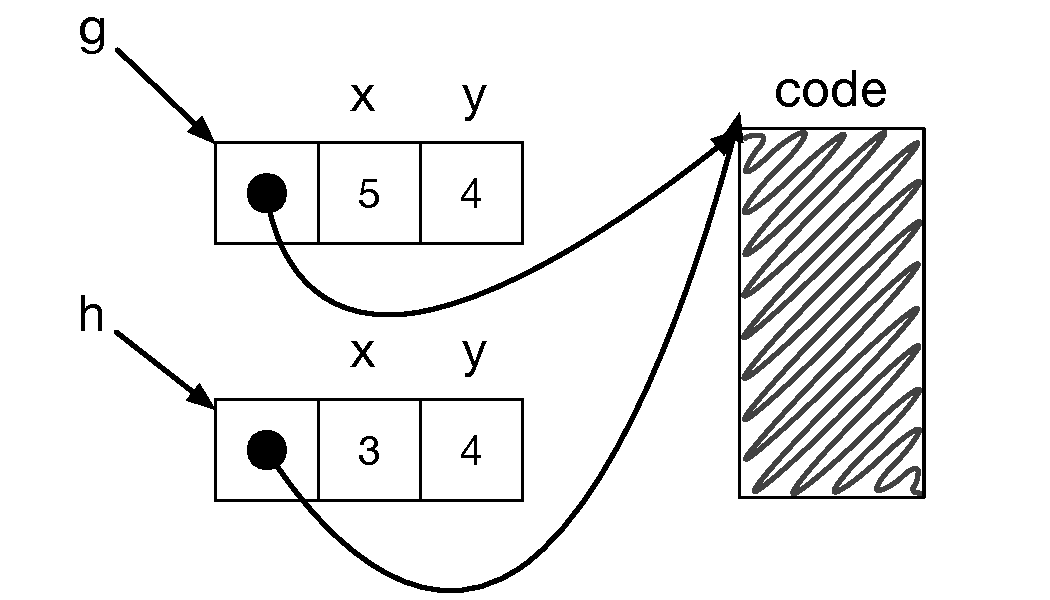
\includegraphics[width=0.6\textwidth]{figs/closures}
\caption{Example closure representation for the \key{lambda}'s
  in Figure~\ref{fig:lexical-scoping}.}
\label{fig:closures}
\end{figure}


\section{Interpreting $R_5$}

Figure~\ref{fig:interp-R5} shows the definitional interpreter for
$R_5$. There are several things to worth noting. First, and most
importantly, the match clause for \key{lambda} saves the current
environment inside the returned \key{lambda}. Then the clause for
\key{app} uses the environment from the \key{lambda}, the
\code{lam-env}, when interpreting the body of the \key{lambda}.  Of
course, the \code{lam-env} environment is extending with the mapping
parameters to argument values. To enable mutual recursion and allow a
unified handling of functions created with \key{lambda} and with
\key{define}, the match clause for \key{program} includes a second
pass over the top-level functions to set their environments to be the
top-level environment.

\begin{figure}[tbp]
\begin{lstlisting}
(define (interp-R5 env)
  (lambda (ast)
    (match ast
       ...
       [`(lambda: ([,xs : ,Ts] ...) : ,rT ,body)
        `(lambda ,xs ,body ,env)]
       [`(define (,f [,xs : ,ps] ...) : ,rt ,body)
        (mcons f `(lambda ,xs ,body))]
       [`(program ,defs ... ,body)
        (let ([top-level (map (interp-R5 '()) defs)])
          (for/list ([b top-level])
                    (set-mcdr! b (match (mcdr b)
                                    [`(lambda ,xs ,body)
                                     `(lambda ,xs ,body ,top-level)])))
          ((interp-R5 top-level) body))]
       [`(,fun ,args ...)
        (define arg-vals (map (interp-R5 env) args))
        (define fun-val ((interp-R5 env) fun))
        (match fun-val
           [`(lambda (,xs ...) ,body ,lam-env)
            (define new-env (append (map cons xs arg-vals) lam-env))
            ((interp-R5 new-env) body)]
           [else (error "interp-R5, expected function, not" fun-val)])]
       )))
\end{lstlisting}
\caption{Interpreter for $R_5$.}
\label{fig:interp-R5}
\end{figure}

\section{Type Checking $R_5$}

Figure~\ref{fig:typecheck-R5} shows how to type check the new
\key{lambda} form. The body of the \key{lambda} is checked in an
environment that includes the current environment (because it is
lexically scoped) and also includes the \key{lambda}'s parameters.  We
require the body's type to match the declared return type.

\begin{figure}[tbp]
\begin{lstlisting}
(define (typecheck-R5 env)
  (lambda (e)
    (match e
      [`(lambda: ([,xs : ,Ts] ...) : ,rT ,body)
       (define new-env (append (map cons xs Ts) env))
       (define bodyT ((typecheck-R5 new-env) body))
       (cond [(equal? rT bodyT)
              `(,@Ts -> ,rT)]
             [else
              (error "mismatch in return type" bodyT rT)])]
      ...
      )))
\end{lstlisting}
\caption{Type checking the \key{lambda}'s in $R_5$.}
\label{fig:typecheck-R5}
\end{figure}


\section{Closure Conversion}

The compiling of lexically-scoped functions into C-style functions is
accomplished in the pass \code{convert-to-closures} that comes after
\code{reveal-functions} and before flatten. This pass needs to treat
regular function calls differently from applying primitive operators,
and \code{reveal-functions} differentiates those two cases for us.

As usual, we shall implement the pass as a recursive function over the
AST. All of the action is in the clauses for \key{lambda} and
\key{app} (function application). We transform a \key{lambda}
expression into an expression that creates a closure, that is, creates
a vector whose first element is a function pointer and the rest of the
elements are the free variables of the \key{lambda}.  The \itm{name}
is a unique symbol generated to identify the function.

\begin{tabular}{lll}
\begin{minipage}{0.4\textwidth}
\begin{lstlisting}
(lambda: (|\itm{ps}| ...) : |\itm{rt}| |\itm{body}|)
\end{lstlisting}
\end{minipage}
&
$\Rightarrow$
&
\begin{minipage}{0.4\textwidth}
\begin{lstlisting}
(vector |\itm{name}| |\itm{fvs}| ...)
\end{lstlisting}
\end{minipage}
\end{tabular}  \\
%
In addition to transforming each \key{lambda} into a \key{vector}, we
must create a top-level function definition for each \key{lambda}, as
shown below.
\begin{lstlisting}
   (define (|\itm{name}| [clos : _] |\itm{ps}| ...)
      (let ([|$\itm{fvs}_1$| (vector-ref clos 1)])
        ...
        (let ([|$\itm{fvs}_n$| (vector-ref clos |$n$|)])
          |\itm{body'}|)...))
\end{lstlisting}
The \code{clos} parameter refers to the closure whereas $\itm{ps}$ are
the normal parameters of the \key{lambda}. The sequence of \key{let}
forms being the free variables to their values obtained from the
closure.

We transform function application into code that retreives the
function pointer from the closure and then calls the function, passing
in the closure as the first argument. We bind $e'$ to a temporary
variable to avoid code duplication.

\begin{tabular}{lll}
\begin{minipage}{0.3\textwidth}
\begin{lstlisting}
(app |$e$| |\itm{es}| ...)
\end{lstlisting}
\end{minipage}
&
$\Rightarrow$
&
\begin{minipage}{0.5\textwidth}
\begin{lstlisting}
(let ([|\itm{tmp}| |$e'$|])
  (app (vector-ref |\itm{tmp}| 0) |\itm{tmp}| |\itm{es'}|))
\end{lstlisting}
\end{minipage}
\end{tabular}  \\

There is also the question of what to do with top-level function
definitions. To maintain a uniform translation of function
application, we turn function references into closures.

\begin{tabular}{lll}
\begin{minipage}{0.3\textwidth}
\begin{lstlisting}
(function-ref |$f$|)
\end{lstlisting}
\end{minipage}
&
$\Rightarrow$
&
\begin{minipage}{0.5\textwidth}
\begin{lstlisting}
(vector (function-ref |$f$|))
\end{lstlisting}
\end{minipage}
\end{tabular}  \\
%
The top-level function definitions need to be updated as well to take
an extra closure parameter.

\section{An Example Translation}
\label{sec:example-lambda}

Figure~\ref{fig:lexical-functions-example} shows the result of closure
conversion for the example program demonstrating lexical scoping that
we discussed at the beginning of this chapter.


\begin{figure}[h]
\begin{minipage}{0.8\textwidth}
\begin{lstlisting}%[basicstyle=\ttfamily\footnotesize]
(program
 (define (f [x : Integer]) : (Integer -> Integer)
    (let ([y 4])
       (lambda: ([z : Integer]) : Integer
          (+ x (+ y z)))))
 (let ([g (f 5)])
   (let ([h (f 3)])
     (+ (g 11) (h 15)))))
\end{lstlisting}
$\Downarrow$
\begin{lstlisting}%[basicstyle=\ttfamily\footnotesize]
(program (type Integer)
  (define (f (x : Integer)) : (Integer -> Integer)
    (let ((y 4))
       (lambda: ((z : Integer)) : Integer
         (+ x (+ y z)))))
   (let ((g (app (function-ref f) 5)))
      (let ((h (app (function-ref f) 3)))
         (+ (app g 11) (app h 15)))))
\end{lstlisting}
$\Downarrow$
\begin{lstlisting}%[basicstyle=\ttfamily\footnotesize]
(program (type Integer)
  (define (f (clos.1 : _) (x : Integer)) : (Integer -> Integer)
     (let ((y  4))
        (vector (function-ref lam.1) x y)))
  (define (lam.1 (clos.2 : _) (z : Integer)) : Integer
     (let ((x (vector-ref clos.2 1)))
        (let ((y (vector-ref clos.2 2)))
           (+ x (+ y z)))))
   (let ((g (let ((t.1 (vector (function-ref f))))
              (app (vector-ref t.1 0) t.1 5))))
      (let ((h (let ((t.2 (vector  (function-ref f))))
                 (app (vector-ref t.2 0) t.2 3))))
         (+ (let ((t.3  g)) (app (vector-ref t.3 0) t.3 11))
            (let ((t.4  h)) (app (vector-ref t.4 0) t.4 15))))))
\end{lstlisting}
\end{minipage}

\caption{Example of closure conversion.}
\label{fig:lexical-functions-example}
\end{figure}


%%%%%%%%%%%%%%%%%%%%%%%%%%%%%%%%%%%%%%%%%%%%%%%%%%%%%%%%%%%%%%%%%%%%%%%%%%%%%%%%
\chapter{Dynamic Typing}
\label{ch:type-dynamic}

In this chapter we discuss the compilation of a dynamically typed
language, named $R_7$, that is a subset of the Racket language. (In
the previous chapters we have studied subsets of the \emph{Typed}
Racket language.) In dynamically typed languages, an expression may
produce values of differing type. Consider the following example with
a conditional expression that may return a Boolean or an integer
depending on the input to the program.
\begin{lstlisting}
   (not (if (eq? (read) 1) #f 0))
\end{lstlisting}
Languages that allow expressions to produce different kinds of values
are called \emph{polymorphic}, and there are many kinds of
polymorphism, such as subtype polymorphism~\citep{Cardelli:1985kx} and
parametric polymorphism (Chapter~\ref{ch:parametric-polymorphism}).

Another characteristic of dynamically typed languages is that
primitive operations, such as \code{not}, are often defined to operate
on many different types of values. In fact, in Racket, the \code{not}
operator produces a result for any kind of value: given \code{\#f} it
returns \code{\#t} and given anything else it returns \code{\#f}.
Furthermore, even when primitive operations restrict their inputs to
values of a certain type, this restriction is enforced at runtime
instead of during compilation. For example, the following vector
reference results in a run-time contract violation.
\begin{lstlisting}
   (vector-ref (vector 42) #t)
\end{lstlisting}

Let us consider how we might compile untyped Racket to x86, thinking
about the first example above. Our bit-level representation of the
Boolean \code{\#f} is zero and similarly for the integer \code{0}.
However, \code{(not \#f)} should produce \code{\#t} whereas \code{(not
  0)} should produce \code{\#f}. Furthermore, the behavior of
\code{not}, in general, cannot be determined at compile time, but
depends on the runtime type of its input, as in the example above that
depends on the result of \code{(read)}.

The way around this problem is to include information about a value's
runtime type in the value itself, so that this information can be
inspected by operators such as \code{not}.  In particular, we shall
steal the 3 right-most bits from our 64-bit values to encode the
runtime type.  We shall use $001$ to identify integers, $100$ for
Booleans, $010$ for vectors, $011$ for procedures, and $101$ for the
void value. We shall refer to these 3 bits as the \emph{tag} and we
define the following auxilliary function.
\begin{align*}
\itm{tagof}(\key{Integer}) &= 001 \\
\itm{tagof}(\key{Boolean}) &= 100 \\
\itm{tagof}((\key{Vector} \ldots)) &= 010 \\
\itm{tagof}((\key{Vectorof} \ldots)) &= 010 \\
\itm{tagof}((\ldots \key{->} \ldots)) &= 011 \\
\itm{tagof}(\key{Void}) &= 101
\end{align*}
(We shall say more about the new \key{Vectorof} type shortly.)
This stealing of 3 bits comes at some
price: our integers are reduced to ranging from $-2^{60}$ to
$2^{60}$. The stealing does not adversely affect vectors and
procedures because those values are addresses, and our addresses are
8-byte aligned so the rightmost 3 bits are unused, they are always
$000$. Thus, we do not lose information by overwriting the rightmost 3
bits with the tag and we can simply zero-out the tag to recover the
original address.

In some sense, these tagged values are a new kind of value.  Indeed,
we can extend our \emph{typed} language with tagged values by adding a
new type to classify them, called \key{Any}, and with operations for
creating and using tagged values, creating the $R_6$ language defined
in Section~\ref{sec:r6-lang}. Thus, $R_6$ provides the fundamental
support for polymorphism and runtime types that we need to support
dynamic typing.

We shall implement our untyped language $R_7$ by compiling it to
$R_6$. We define $R_7$ in Section~\ref{sec:r7-lang} and describe the
compilation of $R_6$ and $R_7$ in the remainder of this chapter.

\section{The $R_6$ Language: Typed Racket $+$ \key{Any}}
\label{sec:r6-lang}

\begin{figure}[tp]
\centering
\fbox{
\begin{minipage}{0.97\textwidth}
\[
\begin{array}{lcl}
  \Type &::=& \gray{\key{Integer} \mid \key{Boolean}
     \mid (\key{Vector}\;\Type^{+}) \mid (\key{Vectorof}\;\Type) \mid \key{Void}} \\
    &\mid& \gray{(\Type^{*} \; \key{->}\; \Type)} \mid \key{Any} \\
  \FType &::=& \key{Integer} \mid \key{Boolean} \mid (\key{Vectorof}\;\key{Any})
     \mid (\key{Any}^{*} \; \key{->}\; \key{Any})\\
  \itm{cmp} &::= & \key{eq?} \mid \key{<} \mid \key{<=} \mid \key{>} \mid \key{>=} \\
  \Exp &::=& \gray{\Int \mid (\key{read}) \mid (\key{-}\;\Exp)
     \mid (\key{+} \; \Exp\;\Exp)}  \\
    &\mid&  \gray{\Var \mid \LET{\Var}{\Exp}{\Exp}} \\
    &\mid& \gray{\key{\#t} \mid \key{\#f} \mid
           (\key{and}\;\Exp\;\Exp) \mid (\key{not}\;\Exp)} \\
    &\mid& \gray{(\itm{cmp}\;\Exp\;\Exp) \mid \IF{\Exp}{\Exp}{\Exp}} \\
    &\mid& \gray{(\key{vector}\;\Exp^{+}) \mid
          (\key{vector-ref}\;\Exp\;\Int)} \\
    &\mid& \gray{(\key{vector-set!}\;\Exp\;\Int\;\Exp)\mid (\key{void})} \\
    &\mid& \gray{(\Exp \; \Exp^{*})
    \mid (\key{lambda:}\; ([\Var \key{:} \Type]^{*}) \key{:} \Type \; \Exp)} \\
  & \mid & (\key{inject}\; \Exp \; \FType) \mid (\key{project}\;\Exp\;\FType) \\
  & \mid & (\key{boolean?}\;\Exp) \mid (\key{integer?}\;\Exp)\\
  & \mid & (\key{vector?}\;\Exp) \mid (\key{procedure?}\;\Exp) \mid (\key{void?}\;\Exp) \\
  \Def &::=& \gray{(\key{define}\; (\Var \; [\Var \key{:} \Type]^{*}) \key{:} \Type \; \Exp)} \\
  R_6 &::=& \gray{(\key{program} \; \Def^{*} \; \Exp)}
\end{array}
\]
\end{minipage}
}
\caption{Syntax of $R_6$, extending $R_5$ with \key{Any}.}
\label{fig:r6-syntax}
\end{figure}

The syntax of $R_6$ is defined in Figure~\ref{fig:r6-syntax}.  The
$(\key{inject}\; e\; T)$ form converts the value produced by
expression $e$ of type $T$ into a tagged value.  The
$(\key{project}\;e\;T)$ form converts the tagged value produced by
expression $e$ into a value of type $T$ or else halts the program if
the type tag does not match $T$. Note that in both \key{inject} and
\key{project}, the type $T$ is restricted to the flat types $\FType$,
which simplifies the implementation and corresponds with what is
needed for compiling untyped Racket. The type predicates,
$(\key{boolean?}\,e)$ etc., expect a tagged value and return \key{\#t}
if the tag corresponds to the predicate, and return \key{\#t}
otherwise.
%
The type checker for $R_6$ is given in Figure~\ref{fig:typecheck-R6}.

\begin{figure}[tbp]
\begin{lstlisting}[basicstyle=\ttfamily\footnotesize]
(define type-predicates
  (set 'boolean? 'integer? 'vector? 'procedure?))

(define (typecheck-R6 env)
  (lambda (e)
    (define recur (typecheck-R6 env))
    (match e
       [`(inject ,(app recur new-e e-ty) ,ty)
        (cond
         [(equal? e-ty ty)
          (values `(inject ,new-e ,ty) 'Any)]
         [else
          (error "inject expected ~a to have type ~a" e ty)])]
       [`(project ,(app recur new-e e-ty) ,ty)
        (cond
         [(equal? e-ty 'Any)
          (values `(project ,new-e ,ty) ty)]
         [else
          (error "project expected ~a to have type Any" e)])]
       [`(,pred ,e) #:when (set-member? type-predicates pred)
        (define-values (new-e e-ty) (recur e))
        (cond
         [(equal? e-ty 'Any)
          (values `(,pred ,new-e) 'Boolean)]
         [else
          (error "predicate expected arg of type Any, not" e-ty)])]
       [`(vector-ref ,(app recur e t) ,i)
        (match t
          [`(Vector ,ts ...) ...]
          [`(Vectorof ,t)
           (unless (exact-nonnegative-integer? i)
             (error 'type-check "invalid index ~a" i))
           (values `(vector-ref ,e ,i) t)]
          [else (error "expected a vector in vector-ref, not" t)])]
       [`(vector-set! ,(app recur e-vec^ t-vec) ,i
                       ,(app recur e-arg^ t-arg))
        (match t-vec
          [`(Vector ,ts ...) ...]
          [`(Vectorof ,t)
           (unless (exact-nonnegative-integer? i)
             (error 'type-check "invalid index ~a" i))
           (unless (equal? t t-arg)
             (error 'type-check "type mismatch in vector-set! ~a ~a"
                    t t-arg))
           (values `(vector-set! ,e-vec^
                                           ,i
                                           ,e-arg^) 'Void)]
          [else (error 'type-check
                       "expected a vector in vector-set!, not ~a"
                       t-vec)])]
        ...
      )))
\end{lstlisting}
\caption{Type checker for the $R_6$ language.}
\label{fig:typecheck-R6}
\end{figure}

% to do: add rules for vector-ref, etc. for Vectorof


%Also, \key{eq?} is extended to operate on values of type \key{Any}.

Figure~\ref{fig:interp-R6} shows the definitional interpreter
for $R_6$.

\begin{figure}[tbp]
\begin{lstlisting}
(define primitives (set 'boolean? ...))

(define (interp-op op)
  (match op
     ['boolean? (lambda (v)
                  (match v
                     [`(tagged ,v1 Boolean) #t]
                     [else #f]))]
     ...))

(define (interp-R6 env)
  (lambda (ast)
    (match ast
       [`(inject ,e ,t)
        `(tagged ,((interp-R6 env) e) ,t)]
       [`(project ,e ,t2)
        (define v ((interp-R6 env) e))
        (match v
           [`(tagged ,v1 ,t1)
            (cond [(equal? t1 t2)
                   v1]
                  [else
                   (error "in project, type mismatch" t1 t2)])]
           [else
            (error "in project, expected tagged value" v)])]
       ...)))
\end{lstlisting}
\caption{Interpreter for $R_6$.}
\label{fig:interp-R6}
\end{figure}


\section{The $R_7$ Language: Untyped Racket}
\label{sec:r7-lang}

\begin{figure}[tp]
\centering
\fbox{
\begin{minipage}{0.97\textwidth}
\[
\begin{array}{rcl}
  \itm{cmp} &::= & \key{eq?} \mid \key{<} \mid \key{<=} \mid \key{>} \mid \key{>=} \\
\Exp &::=& \Int \mid (\key{read}) \mid (\key{-}\;\Exp) \mid (\key{+} \; \Exp\;\Exp)  \\
     &\mid&  \Var \mid \LET{\Var}{\Exp}{\Exp} \\
     &\mid& \key{\#t} \mid \key{\#f} \mid
      (\key{and}\;\Exp\;\Exp) \mid (\key{not}\;\Exp) \\
     &\mid& (\itm{cmp}\;\Exp\;\Exp) \mid \IF{\Exp}{\Exp}{\Exp} \\
     &\mid& (\key{vector}\;\Exp^{+}) \mid
      (\key{vector-ref}\;\Exp\;\Exp) \\
  &\mid& (\key{vector-set!}\;\Exp\;\Exp\;\Exp) \mid (\key{void}) \\
  &\mid& (\Exp \; \Exp^{*}) \mid (\key{lambda}\; (\Var^{*}) \; \Exp) \\
  \Def &::=& (\key{define}\; (\Var \; \Var^{*}) \; \Exp) \\
R_7  &::=& (\key{program} \; \Def^{*}\; \Exp)
\end{array}
\]
\end{minipage}
}
\caption{Syntax of $R_7$, an untyped language (a subset of Racket).}
\label{fig:r7-syntax}
\end{figure}

The syntax of $R_7$, our subset of Racket, is defined in
Figure~\ref{fig:r7-syntax}.
%
The definitional interpreter for $R_7$ is given in
Figure~\ref{fig:interp-R7}.

\begin{figure}[tbp]
\begin{lstlisting}[basicstyle=\ttfamily\footnotesize]
(define (get-tagged-type v) (match v [`(tagged ,v1 ,ty) ty]))

(define (valid-op? op) (member op '(+ - and or not)))

(define (interp-r7 env)
  (lambda (ast)
    (define recur (interp-r7 env))
    (match ast
      [(? symbol?) (lookup ast env)]
      [(? integer?) `(inject ,ast Integer)]
      [#t `(inject #t Boolean)]
      [#f `(inject #f Boolean)]
      [`(read) `(inject ,(read-fixnum) Integer)]
      [`(lambda (,xs ...) ,body)
       `(inject (lambda ,xs ,body ,env) (,@(map (lambda (x) 'Any) xs) -> Any))]
      [`(define (,f ,xs ...) ,body)
       (mcons f `(lambda ,xs ,body))]
      [`(program ,ds ... ,body)
       (let ([top-level (map (interp-r7 '()) ds)])
         (for/list ([b top-level])
           (set-mcdr! b (match (mcdr b)
                          [`(lambda ,xs ,body)
                           `(inject (lambda ,xs ,body ,top-level)
                                    (,@(map (lambda (x) 'Any) xs) -> Any))])))
         ((interp-r7 top-level) body))]
      [`(vector ,(app recur elts) ...)
       (define tys (map get-tagged-type elts))
       `(inject ,(apply vector elts) (Vector ,@tys))]
      [`(vector-set! ,(app recur v1) ,n ,(app recur v2))
         (match v1
           [`(inject ,vec ,ty)
             (vector-set! vec n v2)
            `(inject (void) Void)])]
      [`(vector-ref ,(app recur v) ,n)
       (match v [`(inject ,vec ,ty) (vector-ref vec n)])]
      [`(let ([,x ,(app recur v)]) ,body)
       ((interp-r7 (cons (cons x v) env)) body)]
      [`(,op ,es ...) #:when (valid-op? op)
       (interp-r7-op op (map recur es))]
      [`(eq? ,(app recur l) ,(app recur r))
       `(inject ,(equal? l r) Boolean)]
      [`(if ,(app recur q) ,t ,f)
       (match q
         [`(inject #f Boolean) (recur f)]
         [else (recur t)])]
      [`(,(app recur f-val) ,(app recur vs) ...)
       (match f-val
         [`(inject (lambda (,xs ...) ,body ,lam-env) ,ty)
          (define new-env (append (map cons xs vs) lam-env))
          ((interp-r7 new-env) body)]
         [else (error "interp-r7, expected function, not" f-val)])])))
\end{lstlisting}
\caption{Interpreter for the $R_7$ language.}
\label{fig:interp-R7}
\end{figure}



\section{Compiling $R_6$}
\label{sec:compile-r6}

Most of the compiler passes only require straightforward changes.  The
interesting part is in instruction selection.

\paragraph{Inject}

We recommend compiling an \key{inject} as follows if the type is
\key{Integer} or \key{Boolean}.  The \key{salq} instruction shifts the
destination to the left by the number of bits specified by the source
($2$) and it preserves the sign of the integer. We use the \key{orq}
instruction to combine the tag and the value to form the tagged value.
\\
\begin{tabular}{lll}
\begin{minipage}{0.4\textwidth}
\begin{lstlisting}
(assign |\itm{lhs}| (inject |$e$| |$T$|))
\end{lstlisting}
\end{minipage}
&
$\Rightarrow$
&
\begin{minipage}{0.5\textwidth}
\begin{lstlisting}
(movq |$e'$| |\itm{lhs}'|)
(salq (int 2) |\itm{lhs}'|)
(orq (int |$\itm{tagof}(T)$|) |\itm{lhs}'|)
\end{lstlisting}
\end{minipage}
\end{tabular}  \\
The instruction selection for vectors and procedures is different
because their is no need to shift them to the left. The rightmost 3
bits are already zeros as described above. So we combine the value and
the tag using
\key{orq}.  \\
\begin{tabular}{lll}
\begin{minipage}{0.4\textwidth}
\begin{lstlisting}
(assign |\itm{lhs}| (inject |$e$| |$T$|))
\end{lstlisting}
\end{minipage}
&
$\Rightarrow$
&
\begin{minipage}{0.5\textwidth}
\begin{lstlisting}
(movq |$e'$| |\itm{lhs}'|)
(orq (int |$\itm{tagof}(T)$|) |\itm{lhs}'|)
\end{lstlisting}
\end{minipage}
\end{tabular}  \\

\paragraph{Project}


The instruction selection for \key{project} is a bit more involved.
Like \key{inject}, the instructions are different depending on whether
the type $T$ is a pointer (vector or procedure) or not (Integer or
Boolean). The following shows the instruction selection for Integer
and Boolean.  We first check to see if the tag on the tagged value
matches the tag of the target type $T$. If not, we halt the program by
calling the \code{exit} function. If we have a match, we need to
produce an untagged value by shifting it to the right by 2 bits.
%
\\
\begin{tabular}{lll}
\begin{minipage}{0.4\textwidth}
\begin{lstlisting}
(assign |\itm{lhs}| (project |$e$| |$T$|))
\end{lstlisting}
\end{minipage}
&
$\Rightarrow$
&
\begin{minipage}{0.5\textwidth}
\begin{lstlisting}
(movq |$e'$| |\itm{lhs}'|)
(andq (int 3) |\itm{lhs}'|)
(if (eq? |\itm{lhs}'| (int |$\itm{tagof}(T)$|))
    ((movq |$e'$| |\itm{lhs}'|)
     (sarq (int 2) |\itm{lhs}'|))
    ((callq exit)))
\end{lstlisting}
\end{minipage}
\end{tabular}  \\
%
The case for vectors and procedures begins in a similar way, checking
that the runtime tag matches the target type $T$ and exiting if there
is a mismatch. However, the way in which we convert the tagged value
to a value is different, as there is no need to shift. Instead we need
to zero-out the rightmost 2 bits. We accomplish this by creating the
bit pattern $\ldots 0011$, applying \code{notq} to obtain $\ldots
1100$, and then applying \code{andq} with the tagged value get the
desired result. \\
%
\begin{tabular}{lll}
\begin{minipage}{0.4\textwidth}
\begin{lstlisting}
(assign |\itm{lhs}| (project |$e$| |$T$|))
\end{lstlisting}
\end{minipage}
&
$\Rightarrow$
&
\begin{minipage}{0.5\textwidth}
\begin{lstlisting}
(movq |$e'$| |\itm{lhs}'|)
(andq (int 3) |\itm{lhs}'|)
(if (eq? |\itm{lhs}'| (int |$\itm{tagof}(T)$|))
    ((movq (int 3) |\itm{lhs}'|)
     (notq |\itm{lhs}'|)
     (andq |$e'$| |\itm{lhs}'|))
    ((callq exit)))
\end{lstlisting}
\end{minipage}
\end{tabular}  \\

\paragraph{Type Predicates} We leave it to the reader to
devise a sequence of instructions to implement the type predicates
\key{boolean?}, \key{integer?}, \key{vector?}, and \key{procedure?}.

\section{Compiling $R_7$ to $R_6$}
\label{sec:compile-r7}

Figure~\ref{fig:compile-r7-r6} shows the compilation of many of the
$R_7$ forms into $R_6$. An important invariant of this pass is that
given a subexpression $e$ of $R_7$, the pass will produce an
expression $e'$ of $R_6$ that has type \key{Any}. For example, the
first row in Figure~\ref{fig:compile-r7-r6} shows the compilation of
the Boolean \code{\#t}, which must be injected to produce an
expression of type \key{Any}.
%
The second row of Figure~\ref{fig:compile-r7-r6}, the compilation of
addition, is representative of compilation for many operations: the
arguments have type \key{Any} and must be projected to \key{Integer}
before the addition can be performed.
%
The compilation of \key{lambda} (third row of
Figure~\ref{fig:compile-r7-r6}) shows what happens when we need to
produce type annotations, we simply use \key{Any}.
%
The compilation of \code{if}, \code{eq?}, and \code{and} all
demonstrate how this pass has to account for some differences in
behavior between $R_7$ and $R_6$. The $R_7$ language is more
permissive than $R_6$ regarding what kind of values can be used in
various places. For example, the condition of an \key{if} does not
have to be a Boolean. Similarly, the arguments of \key{and} do not
need to be Boolean. For \key{eq?}, the arguments need not be of the
same type.

\begin{figure}[tbp]
\centering
\begin{tabular}{|lll|} \hline
\begin{minipage}{0.25\textwidth}
\begin{lstlisting}
#t
\end{lstlisting}
\end{minipage}
&
$\Rightarrow$
&
\begin{minipage}{0.6\textwidth}
\begin{lstlisting}
(inject #t Boolean)
\end{lstlisting}
\end{minipage}
\\[2ex]\hline
\begin{minipage}{0.25\textwidth}
\begin{lstlisting}
(+ |$e_1$| |$e_2$|)
\end{lstlisting}
\end{minipage}
&
$\Rightarrow$
&
\begin{minipage}{0.6\textwidth}
\begin{lstlisting}
(inject
   (+ (project |$e'_1$| Integer)
      (project |$e'_2$| Integer))
   Integer)
\end{lstlisting}
\end{minipage}
\\[2ex]\hline
\begin{minipage}{0.25\textwidth}
\begin{lstlisting}
(lambda (|$x_1 \ldots$|) |$e$|)
\end{lstlisting}
\end{minipage}
&
$\Rightarrow$
&
\begin{minipage}{0.6\textwidth}
\begin{lstlisting}
(inject (lambda: ([|$x_1$|:Any]|$\ldots$|):Any |$e'$|)
        (Any|$\ldots$|Any -> Any))
\end{lstlisting}
\end{minipage}
\\[2ex]\hline
\begin{minipage}{0.25\textwidth}
\begin{lstlisting}
(app |$e_0$| |$e_1 \ldots e_n$|)
\end{lstlisting}
\end{minipage}
&
$\Rightarrow$
&
\begin{minipage}{0.6\textwidth}
\begin{lstlisting}
(app (project |$e'_0$| (Any|$\ldots$|Any -> Any))
   |$e'_1 \ldots e'_n$|)
\end{lstlisting}
\end{minipage}
\\[2ex]\hline
\begin{minipage}{0.25\textwidth}
\begin{lstlisting}
(vector-ref |$e_1$| |$e_2$|)
\end{lstlisting}
\end{minipage}
&
$\Rightarrow$
&
\begin{minipage}{0.6\textwidth}
\begin{lstlisting}
(let ([tmp1 (project |$e'_1$| (Vectorof Any))])
  (let ([tmp2 (project |$e'_2$| Integer)])
     (vector-ref tmp1 tmp2)))
\end{lstlisting}
\end{minipage}
\\[2ex]\hline
\begin{minipage}{0.25\textwidth}
\begin{lstlisting}
(if |$e_1$| |$e_2$| |$e_3$|)
\end{lstlisting}
\end{minipage}
&
$\Rightarrow$
&
\begin{minipage}{0.6\textwidth}
\begin{lstlisting}
(if (eq? |$e'_1$| (inject #f Boolean))
   |$e'_3$|
   |$e'_2$|)
\end{lstlisting}
\end{minipage}
\\[2ex]\hline
\begin{minipage}{0.25\textwidth}
\begin{lstlisting}
(eq? |$e_1$| |$e_2$|)
\end{lstlisting}
\end{minipage}
&
$\Rightarrow$
&
\begin{minipage}{0.6\textwidth}
\begin{lstlisting}
(inject (eq? |$e'_1$| |$e'_2$|) Boolean)
\end{lstlisting}
\end{minipage}
\\[2ex]\hline
\begin{minipage}{0.25\textwidth}
\begin{lstlisting}
(and |$e_1$| |$e_2$|)
\end{lstlisting}
\end{minipage}
&
$\Rightarrow$
&
\begin{minipage}{0.6\textwidth}
\begin{lstlisting}
(let ([tmp |$e'_1$|])
   (if (eq? tmp (inject #f Boolean))
      tmp
      |$e'_2$|))
\end{lstlisting}
\end{minipage} \\\hline
\end{tabular}  \\

\caption{Compiling $R_7$ to $R_6$.}
\label{fig:compile-r7-r6}
\end{figure}

%%%%%%%%%%%%%%%%%%%%%%%%%%%%%%%%%%%%%%%%%%%%%%%%%%%%%%%%%%%%%%%%%%%%%%%%%%%%%%%%
\chapter{Gradual Typing}
\label{ch:gradual-typing}

This chapter will be based on the ideas of \citet{Siek:2006bh}.

%%%%%%%%%%%%%%%%%%%%%%%%%%%%%%%%%%%%%%%%%%%%%%%%%%%%%%%%%%%%%%%%%%%%%%%%%%%%%%%%
\chapter{Parametric Polymorphism}
\label{ch:parametric-polymorphism}

This chapter may be based on ideas from \citet{Cardelli:1984aa},
\citet{Leroy:1992qb}, \citet{Shao:1997uj}, or \citet{Harper:1995um}.





%%%%%%%%%%%%%%%%%%%%%%%%%%%%%%%%%%%%%%%%%%%%%%%%%%%%%%%%%%%%%%%%%%%%%%%%%%%%%%%%
\chapter{High-level Optimization}
\label{ch:high-level-optimization}

This chapter will present a procedure inlining pass based on the
algorithm of \citet{Waddell:1997fk}.


%%%%%%%%%%%%%%%%%%%%%%%%%%%%%%%%%%%%%%%%%%%%%%%%%%%%%%%%%%%%%%%%%%%%%%%%%%%%%%%%
\chapter{Appendix}

\section{Interpreters}
\label{appendix:interp}

We provide several interpreters in the \key{interp.rkt} file.  The
\key{interp-scheme} function takes an AST in one of the Racket-like
languages considered in this book ($R_1, R_2, \ldots$) and interprets
the program, returning the result value.  The \key{interp-C} function
interprets an AST for a program in one of the C-like languages ($C_0,
C_1, \ldots$), and the \code{interp-x86} function interprets an AST
for an x86 program.

\section{Utility Functions}
\label{appendix:utilities}

The utility function described in this section can be found in the
\key{utilities.rkt} file.

The \key{read-program} function takes a file path and parses that file
(it must be a Racket program) into an abstract syntax tree (as an
S-expression) with a \key{program} AST at the top.

The \key{assert} function displays the error message \key{msg} if the
Boolean \key{bool} is false.
\begin{lstlisting}
(define (assert msg bool) ...)
\end{lstlisting}

The \key{lookup} function ...

The \key{map2} function ...


\subsection{Graphs}

\begin{itemize}
\item The \code{make-graph} function takes a list of vertices
  (symbols) and returns a graph.

\item The \code{add-edge} function takes a graph and two vertices and
  adds an edge to the graph that connects the two vertices. The graph
  is updated in-place. There is no return value for this function.

\item The \code{adjacent} function takes a graph and a vertex and
  returns the set of vertices that are adjacent to the given
  vertex. The return value is a Racket \code{hash-set} so it can be
  used with functions from the \code{racket/set} module.

\item The \code{vertices} function takes a graph and returns the list
  of vertices in the graph.
\end{itemize}

\subsection{Testing}

The \key{interp-tests} function takes a compiler name (a string), a
description of the passes, an interpreter for the source language, a
test family name (a string), and a list of test numbers, and runs the
compiler passes and the interpreters to check whether the passes
correct. The description of the passes is a list with one entry per
pass.  An entry is a list with three things: a string giving the name
of the pass, the function that implements the pass (a translator from
AST to AST), and a function that implements the interpreter (a
function from AST to result value) for the language of the output of
the pass.  The interpreters from Appendix~\ref{appendix:interp} make a
good choice.  The \key{interp-tests} function assumes that the
subdirectory \key{tests} has a bunch of Scheme programs whose names
all start with the family name, followed by an underscore and then the
test number, ending in \key{.scm}. Also, for each Scheme program there
is a file with the same number except that it ends with \key{.in} that
provides the input for the Scheme program.
\begin{lstlisting}
(define (interp-tests name passes test-family test-nums) ...
\end{lstlisting}

The compiler-tests function takes a compiler name (a string) a
description of the passes (see the comment for \key{interp-tests}) a
test family name (a string), and a list of test numbers (see the
comment for interp-tests), and runs the compiler to generate x86 (a
\key{.s} file) and then runs gcc to generate machine code.  It runs
the machine code and checks that the output is 42.
\begin{lstlisting}
(define (compiler-tests name passes test-family test-nums) ...)
\end{lstlisting}

The compile-file function takes a description of the compiler passes
(see the comment for \key{interp-tests}) and returns a function that,
given a program file name (a string ending in \key{.scm}), applies all
of the passes and writes the output to a file whose name is the same
as the program file name but with \key{.scm} replaced with \key{.s}.
\begin{lstlisting}
(define (compile-file passes)
  (lambda (prog-file-name) ...))
\end{lstlisting}

\section{x86 Instruction Set Quick-Reference}
\label{sec:x86-quick-reference}


Table~\ref{tab:x86-instr} lists some x86 instructions and what they
do. We write $A \to B$ to mean that the value of $A$ is written into
location $B$.  Address offsets are given in bytes. The instruction
arguments $A, B, C$ can be immediate constants (such as $\$4$),
registers (such as $\%rax$), or memory references (such as
$-4(\%ebp)$). Most x86 instructions only allow at most one memory
reference per instruction.  Other operands must be immediates or
registers.


\begin{table}[tbp]
  \centering
\begin{tabular}{l|l}
\textbf{Instruction} & \textbf{Operation} \\ \hline
\texttt{addq} $A$, $B$ &  $A + B \to B$\\
\texttt{negq} $A$ & $- A \to A$ \\
\texttt{subq} $A$, $B$ &  $B - A \to B$\\
\texttt{callq} $L$ & Pushes the return address and jumps to label $L$ \\
\texttt{callq} *$A$ & Calls the function at the address $A$. \\
%\texttt{leave} & $\texttt{ebp} \to \texttt{esp};$ \texttt{popl \%ebp} \\
\texttt{retq} & Pops the return address and jumps to it \\
\texttt{popq} $A$ & $*\mathtt{rsp} \to A; \mathtt{rsp} + 8 \to \mathtt{rsp}$ \\
\texttt{pushq} $A$ & $\texttt{rsp} - 8 \to \texttt{rsp}; A \to *\texttt{rsp}$\\
\texttt{leaq} $A$,$B$ & $A \to B$ ($C$ must be a register) \\
\texttt{cmpq} $A$, $B$ & compare $A$ and $B$ and set flag \\
\texttt{je} $L$ & \multirow{5}{3.7in}{Jump to label $L$ if the flag matches
   the condition code, otherwise go to the next instructions.
  The condition codes are \key{e} for ``equal'',
  \key{l} for ``less'', \key{le} for ``less or equal'', \key{g}
  for ``greater'', and \key{ge} for ``greater or equal''.} \\
\texttt{jl} $L$ & \\
\texttt{jle} $L$ & \\
\texttt{jg} $L$ & \\
\texttt{jge} $L$ & \\
\texttt{jmp} $L$ & Jump to label $L$ \\
\texttt{movq} $A$, $B$ &  $A \to B$ \\
\texttt{movzbq} $A$, $B$ &
  \multirow{3}{3.7in}{$A \to B$, \text{where } $A$ is a single-byte register
  (e.g., \texttt{al} or \texttt{cl}), $B$ is a 8-byte register,
  and the extra bytes of $B$ are set to zero.} \\
 & \\
 & \\
\texttt{notq} $A$ & $\sim A \to A$ \qquad (bitwise complement)\\
\texttt{orq} $A$, $B$ & $A | B \to B$ \qquad (bitwise-or)\\
\texttt{andq} $A$, $B$ & $A \& B \to B$ \qquad (bitwise-and)\\
\texttt{salq} $A$, $B$ & $B$ \texttt{<<} $A \to B$ (arithmetic shift left, where $A$ is a constant)\\
\texttt{sarq} $A$, $B$ & $B$ \texttt{>>} $A \to B$ (arithmetic shift right, where $A$ is a constant)\\
\texttt{sete} $A$ & \multirow{5}{3.7in}{If the flag matches the condition code,
   then $1 \to A$, else $0 \to A$. Refer to \texttt{je} above for the
   description of the condition codes. $A$ must be a single byte register
   (e.g., \texttt{al} or \texttt{cl}).} \\
\texttt{setl} $A$ & \\
\texttt{setle} $A$ & \\
\texttt{setg} $A$ & \\
\texttt{setge} $A$ &
\end{tabular}
\vspace{5pt}
  \caption{Quick-reference for the x86 instructions used in this book.}
  \label{tab:x86-instr}
\end{table}



\bibliographystyle{plainnat}
\bibliography{all}

\end{document}

%%  LocalWords:  Dybvig Waddell Abdulaziz Ghuloum Dipanwita Sussman
%%  LocalWords:  Sarkar lcl Matz aa representable Chez Ph Dan's nano
%%  LocalWords:  fk bh Siek plt uq Felleisen Bor Yuh ASTs AST Naur eq
%%  LocalWords:  BNF fixnum datatype arith prog backquote quasiquote
%%  LocalWords:  ast sexp Reynold's reynolds interp cond fx evaluator
%%  LocalWords:  quasiquotes pe nullary unary rcl env lookup gcc rax
%%  LocalWords:  addq movq callq rsp rbp rbx rcx rdx rsi rdi subq nx
%%  LocalWords:  negq pushq popq retq globl Kernighan uniquify lll ve
%%  LocalWords:  allocator gensym alist subdirectory scm rkt tmp lhs
%%  LocalWords:  runtime Liveness liveness undirected Balakrishnan je
%%  LocalWords:  Rosen DSATUR SDO Gebremedhin Omari morekeywords cnd
%%  LocalWords:  fullflexible vertices Booleans Listof Pairof thn els
%%  LocalWords:  boolean typecheck notq cmpq sete movzbq jmp al xorq
%%  LocalWords:  EFLAGS thns elss elselabel endlabel Tuples tuples os
%%  LocalWords:  tuple args lexically leaq Polymorphism msg bool nums
%%  LocalWords:  macosx unix Cormen vec callee xs maxStack numParams
%%  LocalWords:  arg bitwise XOR'd thenlabel immediates optimizations
%%  LocalWords:  deallocating Ungar Detlefs Tene kx FromSpace ToSpace
%%  LocalWords:  Appel Diwan Siebert ptr  fromspace rootstack typedef
%%  LocalWords:  len prev rootlen heaplen setl lt
